%==================================================================
% Ini adalah file utama dari dokumen LaTeX ini
%==================================================================

%% DILARANG EDIT BAGIAN INI
\documentclass[12pt, a4paper, onecolumn, oneside, final]{report}

%%========================================================================
%% INFORMASI YANG WAJIB DIUBAH. PASTIKAN SEMUA COMMAND DIISI DENGAN DATA YANG BENAR
%%========================================================================

\providecommand{\judulid}{Judul Skripsi} %Judul Tugas Akhir Bahasa Indonesia
\providecommand{\judulen}{Thesis Title} %Judul Tugas Akhir Bahasa Inggirs
\providecommand{\penulis}{Abdillah Haidar Mahendro} %Nama Lengkap Mahasiswa 
\providecommand{\nim}{43A87006220068}
\providecommand{\tempattanggallahir}{Jakarta, 17 April 2001}
\providecommand{\jeniskelamin}{Laki-laki}
\providecommand{\alamat}{Jl. Bambu Kuning IX No. 108 RT 02/03 Sepanjang Jaya, Rawalumbu, Bekasi}
\providecommand{\agama}{Islam}
\providecommand{\statuspernikahan}{Belum Menikah}
\providecommand{\nohandphone}{088977664271}
\providecommand{\email}{abdil.haidar17@gmail.com}

\providecommand{\datapribadi}{
    % BUKAN BAGIAN YANG DIEDIT
    \begin{tabular}{@{}p{4cm}rp{8cm}@{}}
        Nama                        & : & {\penulis} \\
        Tempat Tanggal Lahir        & : & {\tempattanggallahir} \\
        Jenis Kelamin               & : & {\jeniskelamin} \\
        Alamat                      & : & {\alamat} \\
        Agama                       & : & {\agama} \\
        Status Perkawinan           & : & {\statuspernikahan} \\
        No. Handphone               & : & {\nohandphone} \\
        Email                       & : & \textcolor{blue}{\underline{\href{mailto:{\email}}{\email}}} \\[0.5cm]
    \end{tabular}
    
    % SILAKAN EDIT DATA PADA BAGIAN INI
    \newcounter{pendidikan}
    \setcounter{pendidikan}{0}
    \begin{tabular}{@{}p{0.5cm}p{3cm}rp{8cm}@{}}
        \multicolumn{4}{@{}l@{}}{\textbf{Riwayat Pendidikan}} \\[0.2cm]
        
        \stepcounter{pendidikan}\arabic{pendidikan}. & Sekolah & : & SDN Karang Tengah 6 Tangerang \\
        & Tahun                                                & : & 2007 - 2009 \\
        & Keterangan                                           & : & Pindah \\[0.3cm]
        
        \stepcounter{pendidikan}\arabic{pendidikan}. & Sekolah & : & SDN Pasir Muncang Caringin \\
        & Tahun                                                & : & 2009 - 2011 \\
        & Keterangan                                           & : & Pindah \\[0.3cm]
        
        \stepcounter{pendidikan}\arabic{pendidikan}. & Sekolah & : & SDN Karang Sari 1 Tangerang \\
        & Tahun                                                & : & 2011 - 2012 \\
        & Keterangan                                           & : & Pindah \\[0.3cm]
    
        \stepcounter{pendidikan}\arabic{pendidikan}. & Sekolah & : & SDN Sepanjang Jaya VIII Bekasi \\
        & Tahun                                                & : & 2012 - 2013 \\
        & Keterangan                                           & : & Lulus Berijazah \\[0.3cm]
    
        \stepcounter{pendidikan}\arabic{pendidikan}. & Sekolah & : & SMPN 2 Bekasi \\
        & Tahun                                                & : & 2013 - 2016 \\
        & Keterangan                                           & : & Lulus Berijazah \\[0.3cm]
        
        \stepcounter{pendidikan}\arabic{pendidikan}. & Sekolah & : & SMK Karya Bhakti 1 Bekasi \\
        & Tahun                                                & : & 2016 - 2019 \\
        & Keterangan                                           & : & Lulus Berijazah \\[0.3cm]
        
        \stepcounter{pendidikan}\arabic{pendidikan}. & Sekolah & : & Universitas Bani Saleh \\
        & Tahun                                                & : & 2022 - Sekarang \\
    \end{tabular}
}

\providecommand{\tipe}{Skripsi} %Tugas Akhir, Karya Ilmiah, Skripsi
\providecommand{\type}{Undergraduate Thesis} %Undergraduate Thesis
\providecommand{\gelar}{Sarjana} %Bisa diganti sesuai dengan gelar mahasiswa (Sarjana / Diplomat)
\providecommand{\gelartingkat}{Strata 1} %Bisa diganti sesuai dengan gelar mahasiswa (Strata 1 / Diploma 3)
\providecommand{\gelarsingkat}{S1} %Bisa diganti sesuai dengan gelar mahasiswa (S1 / D3)
\providecommand{\prodi}{Teknik Informatika} %
\providecommand{\fakultas}{Fakultas Teknologi dan Informasi Digital} %
\providecommand{\universitas}{Universitas Bani Saleh} %

\providecommand{\tglpersetujuan}{06 Juni 2025} %Tanggal di Lembar Persetujuan
\providecommand{\tglpengesahan}{\today} %Tanggal di Lembar Pengesahan
\providecommand{\tglpernyataan}{\today} %Tanggal di Lembar Pernyataan
\providecommand{\tahun}{\the\year{}} %Tahun Proyek Akhir
\providecommand{\takunakademik}{2024/2025} %

\providecommand{\rektor}{Dr. Ns. Desrinah Harahap, M.Kep., Sp.Kep.Mat} %Nama Rektor

\providecommand{\dekan}{Rahmadi, S.Kom., M.Kom.} %Nama Dosen Dekan
\providecommand{\kaprodi}{Zaenal Muttaqin Subekti S.Kom., M.Kom.} %Nama Dosen Kaprodi
\providecommand{\NIPdekan}{1234567890} %NIP Dosen Dekan
\providecommand{\NIPkaprodi}{1234567890} %NIP Dosen Kaprodi

\providecommand{\pembimbingutama}{Abdillah Haidar Mahendro} %Nama Dosen Pembimbing Utama
\providecommand{\pembimbingpendamping}{Abdillah Haidar Mahendro} %Nama Dosen Pembimbing Pendamping
\providecommand{\NIPpembimbingutama}{43A87006220068} %NIP Dosen Pembimbing Utama
\providecommand{\NIPpembimbingpendamping}{43A87006220068} %NIP Dosen Pembimbing Pendamping

\providecommand{\pengujisatu}{Abdillah Haidar Mahendro} %Nama Dosen Penguji 1
\providecommand{\pengujidua}{Abdillah Haidar Mahendro} %Nama Dosen Penguji 2
\providecommand{\pengujitiga}{Abdillah Haidar Mahendro} %Nama Dosen Penguji 3
\providecommand{\NIDNpengujisatu}{43A87006220068} %NIDN Dosen Penguji 1
\providecommand{\NIDNpengujidua}{43A87006220068} %NIDN Dosen Penguji 2
\providecommand{\NIDNpengujitiga}{43A87006220068} %NIDN Dosen Penguji 3

\providecommand{\kota}{Bekasi}

%% Daftar Nama Dosen
%%
%% https://ti.stmik.banisaleh.ac.id/dosen-pages
%==================================================================
% Konfigurasi utama untuk dokumen LaTeX
%==================================================================

%% MENGEDIT BAGIAN INI DAPAT MENGUBAH FORMAT DOKUMEN. HARAP DIHINDARI ATAU LAKUKAN DENGAN HATI-HATI

% Mengatur bahasa dokumen ke Bahasa Indonesia dan encoding karakter
\usepackage[indonesian]{babel}
\usepackage[utf8]{inputenc}
% Pengaturan jarak antar baris dan penyesuaian kotak teks agar rata kiri
\usepackage{setspace}
\usepackage[raggedrightboxes]{ragged2e}
% Paket untuk memasukkan gambar dalam dokumen
\usepackage{graphicx}
\usepackage{float}       % Mengatur posisi gambar dalam teks
% Mengatur indentasi paragraf
\usepackage{indentfirst}  % Memastikan paragraf pertama di setiap section memiliki indentasi
% Paket untuk mengatur indentasi section dan subsection
\usepackage{changepage}
% Mengatur font utama dokumen menjadi Times New Roman
\usepackage{pslatex}
% Pengaturan daftar isi, daftar gambar, dan daftar tabel
\usepackage{chngcntr, tocloft}
% Pengaturan format dan penomoran judul bab
\usepackage{titlesec}
% Pengaturan untuk caption gambar dan tabel
\usepackage[font=small, format=plain, up, textfont=up, tablename=TABEL]{caption}
% \usepackage{caption}
\usepackage{subcaption}
% Pengaturan tabel, multirow, dan ukuran kolom otomatis
\usepackage{tabularx}
\usepackage{multirow}
\usepackage{array}
% Pengaturan margin halaman
\usepackage{geometry}
% Paket untuk notasi matematika
\usepackage{amsmath}
% Untuk halaman berorientasi landscape
\usepackage{rotating}
\usepackage{everypage}
\usepackage{pdflscape}
\usepackage{afterpage}
% Pengaturan untuk list (daftar item dan angka)
\usepackage{enumitem}
% Paket untuk bibliografi menggunakan BibTeX
\usepackage[sort]{natbib}
% Paket untuk tabel yang panjang dan melampaui satu halaman
\usepackage{longtable}
% Paket untuk memasukkan hyperlink dalam dokumen
\usepackage{hyperref}
% Pengaturan label otomatis untuk berbagai elemen (gambar, tabel, persamaan)
\usepackage{cleveref}
% Paket untuk menampilkan kode program
\usepackage{listings}
\usepackage{xcolor}
%paket untuk gambar dengan tikz
\usepackage{tikz}
\usepackage{pgfplots}
\usepackage{pgf-pie}
%untuk if-then
\usepackage{ifthen}
%untuk mesanitasi (sensor) teks
\usepackage{censor}

\usepackage{booktabs}
% Paket untuk menghitung halaman dan referensi
\usepackage{totcount}
\usepackage{lastpage}
\usepackage{refcount}

\graphicspath{{gambar/}} % Menentukan folder default untuk gambar

\setlength\parindent{1cm} % Mengatur jarak indentasi paragraf menjadi 1cm (1 tab)

% Mengatur format penomoran section dan subsection
\renewcommand{\thesection}{\thechapter.\arabic{section}}        % Subsection: 1, 2, 3, ...
\renewcommand{\thesubsection}{\thesection.\arabic{subsection}}  % Subsection: 1.1, 2.1, 3.1, ...

% Pengaturan daftar isi, daftar gambar, dan daftar tabel
\cftsetpnumwidth{1.5em}
\cftsetrmarg{2em}
\setlength{\cftsecnumwidth}{1.5em}
\setlength{\cftsubsecnumwidth}{1.5em}
\renewcommand{\cftchapdotsep}{\cftdotsep}
\setlength{\cftbeforechapskip}{3pt}

% Penyesuaian judul bab dalam daftar isi agar ditampilkan sebagai "BAB"
\renewcommand\cftchappresnum{BAB }
\renewcommand\cftchapaftersnum{}
\newlength\mylen
\settowidth\mylen{\bfseries BAB 1 :\ } % Menyesuaikan lebar penomoran bab
\cftsetindents{chap}{0pt}{\mylen}

% % Pengaturan format dan penomoran judul bab
\titleformat{\chapter}{\doublespacing\fontsize{16pt}{18pt}\bfseries}{\MakeUppercase{\chaptertitlename\ \Roman{chapter}}\filcenter}{0.15cm}{\centering\uppercase}

% % Pengaturan format section dengan adjustwidth otomatis
\titleformat{\section}{\fontsize{14}{16}\bfseries}{\thesection}{0.4cm}{}
\titleformat{\subsection}{\fontsize{14}{16}\bfseries}{\thesubsection}{0.675cm}{}

% Mengatur jarak dan format spacing untuk chapter, section dan subsection
\titlespacing*{\chapter}{0pt}{-1cm}{20pt}
\titlespacing*{\section}{0pt}{10pt}{0cm}
\titlespacing*{\subsection}{2.4em}{10pt}{0cm}

%==================================================================
% CUSTOM ENVIRONMENTS UNTUK INDENTASI SECTION DAN SUBSECTION
%==================================================================

% Environment untuk konten section (indentasi 2.4em)
\newenvironment{sectioncontent}{%
    \begin{adjustwidth}{2.4em}{0pt}%
}{%
    \end{adjustwidth}%
}

% Environment khusus untuk sistematika penulisan
\newenvironment{sistematika}{%
    \begin{sectioncontent}%
    \setlength{\parskip}{0\baselineskip}% Jarak antar paragraf
}{%
    \end{sectioncontent}%
}

% Command untuk membuat item sistematika
% Parameter: {nomor bab romawi}{judul bab}{deskripsi}
\newcommand{\babsistematika}[3]{%
    \noindent\textbf{\makebox[2cm][l]{BAB #1}#2}%\\ Aktifkan bagian ini apabila ingin membuat deskripsi menjadi dalam bentuk paragraf
    % Aktifkan bagian ini apabila ingin membuat deskripsi menjadi dalam bentuk paragraf
    % \hspace{0cm}\noindent\makebox[2cm][l]{}#3\par\vspace{0cm}

    % Aktifkan bagian ini apabila ingin membuat deskripsi tidak dalam bentuk paragraf
    {\leftskip=2cm\noindent#3\par\vspace{0cm}}
}

% Environment untuk konten subsection (indentasi 6.0em)
\newenvironment{subsectioncontent}{%
    \begin{adjustwidth}{6.4em}{0pt}%
}{%
    \end{adjustwidth}%
}

% Environment untuk konten subsubsection (jika diperlukan, indentasi 8.4em)
\newenvironment{subsubsectioncontent}{%
    \begin{adjustwidth}{8.4em}{0pt}%
}{%
    \end{adjustwidth}%
}

% Environment alternatif dengan parameter fleksibel untuk indentasi custom
\newenvironment{customindent}[1]{%
    \begin{adjustwidth}{#1}{0pt}%
}{%
    \end{adjustwidth}%
}

% Macro untuk membuat section dengan konten yang sudah ter-indent otomatis
\newcommand{\indentsection}[2]{%
    \section{#1}%
    \begin{sectioncontent}%
        #2%
    \end{sectioncontent}%
}

% Macro untuk membuat subsection dengan konten yang sudah ter-indent otomatis
\newcommand{\indentsubsection}[2]{%
    \subsection{#1}%
    \begin{subsectioncontent}%
        #2%
    \end{subsectioncontent}%
}

%==================================================================
% PENGATURAN LAINNYA (TETAP SAMA)
%==================================================================

% Menghapus tanda titik dua pada caption
% \captionsetup[figure]{labelsep=space}
% \captionsetup[table]{labelsep=space}
\captionsetup[figure]{
  labelsep=newline,
  singlelinecheck=false,
  justification=centering,
}
\captionsetup[table]{
  labelsep=newline,
  singlelinecheck=false,
  justification=centering,
}

% Mengatur nomor caption gambar dan tabel sesuai bab
\renewcommand{\thefigure}{\arabic{chapter}.\arabic{figure}}
\renewcommand{\thetable}{\arabic{chapter}.\arabic{table}}

% Mengatur hyphenation (pemisahan kata) agar lebih rapi
\tolerance=1
\emergencystretch=\maxdimen
\hyphenpenalty=10000
\hbadness=10000

% Pengaturan margin halaman
\geometry{
    left=4cm,          % Margin kiri
    top=4cm,           % Margin atas
    right=3cm,         % Margin kanan
    bottom=3cm,        % Margin bawah
}

% Pengaturan nomor pada persamaan matematika sesuai bab
%\renewcommand{\theequation}{\arabic{chapter}.\arabic{equation}}
\makeatletter
\renewcommand{\theequation}{\arabic{chapter}.\arabic{equation}}
\renewcommand{\@eqnnum}{\theequation}
\def\tagform@#1{\maketag@@@{#1}} % This line removes the parentheses
\makeatother

% Pengaturan untuk list (daftar item dan angka)
\setlist{nosep} % Menghilangkan jarak antar item dalam list
\newenvironment{packed_enum}{ % Membuat lingkungan untuk daftar bernomor
    \begin{enumerate}[leftmargin=1.5\parindent]
        \setlength{\itemsep}{0pt}
        \setlength{\parskip}{0pt}
        \setlength{\parsep}{0pt}
        }{\end{enumerate}}

\newenvironment{packed_item}{ % Membuat lingkungan untuk daftar berpoin
    \begin{itemize}[leftmargin=1.375\parindent]
        \setlength{\itemsep}{0pt}
        \setlength{\parskip}{0pt}
        \setlength{\parsep}{0pt}
        }{\end{itemize}}

% Paket untuk bibliografi menggunakan BibTeX
\bibliographystyle{newapa} % Ganti dengan apalike jika menggunakan Overleaf

% Pengaturan label otomatis untuk berbagai elemen (gambar, tabel, persamaan)
\crefname{figure}{gambar}{gambar}
\Crefname{figure}{Gambar}{Gambar}
\crefname{table}{tabel}{tabel}
\Crefname{table}{Tabel}{Tabel}
\crefformat{equation}{persamaan~#2#1#3}
\crefname{equation}{persamaan}{persamaan}
\Crefname{equation}{Persamaan}{Persamaan}
\crefname{lstlisting}{kode}{kode}
\Crefname{lstlisting}{Kode}{Kode}

%\AtBeginDocument{\renewcommand{\lstlistingname}{Kode}} 
%\AtBeginDocument{\renewcommand{\thelstlisting}{\thechapter.\arabic{lstlisting}}}
%\AtBeginDocument{\renewcommand{\thelstlisting}{\arabic{chapter}.\arabic{lstlisting}.}}
\AtBeginDocument{\renewcommand{\lstlistingname}{Kode}}
\AtBeginDocument{\renewcommand{\thelstlisting}{\arabic{chapter}.\arabic{lstlisting}}}

\captionsetup[lstlisting]{
  format=plain,
  labelfont=bf,
  justification=centering,
  singlelinecheck=false,
  labelsep=space
}

% Paket untuk menampilkan kode program
\definecolor{codegreen}{rgb}{0,0.6,0}
\definecolor{codegray}{rgb}{0.5,0.5,0.5}
\definecolor{codepurple}{rgb}{0.58,0,0.82}
\definecolor{backcolour}{rgb}{0.95,0.95,0.92}
\lstdefinestyle{mystyle}{
    backgroundcolor=\color{backcolour},   
    commentstyle=\color{codegreen},
    keywordstyle=\color{magenta},
    numberstyle=\tiny\color{codegray},
    stringstyle=\color{codepurple},
    basicstyle=\ttfamily\footnotesize,
    columns=fullflexible,
    breakatwhitespace=false,         
    breaklines=true,                 
    captionpos=b,                    
    keepspaces=true,                 
    numbers=left,                    
    numbersep=5pt,                  
    showspaces=false,                
    showstringspaces=false,
    showtabs=false,                  
    tabsize=2,
    lineskip=-1pt
}
\lstset{style=mystyle}

%paket untuk gambar dengan tikz
\pgfplotsset{compat=1.18}
\usetikzlibrary{shapes.geometric, arrows}
\tikzstyle{startstop} = [rectangle, rounded corners, minimum width=3cm, minimum height=1cm,text centered, draw=black, fill=red!30]
\tikzstyle{process} = [rectangle, minimum width=3cm, minimum height=1cm, text centered, draw=black, fill=orange!30]
\tikzstyle{decision} = [diamond, minimum width=3cm, minimum height=1cm, text centered, draw=black, fill=green!30]
\tikzstyle{arrow} = [thick,->,>=stealth]

% Mendaftarkan counter untuk berbagai elemen
\regtotcounter{table}       % Counter untuk tabel
\regtotcounter{figure}      % Counter untuk gambar

% Counter custom untuk lampiran dan pustaka
\newcounter{lampiran}
\regtotcounter{lampiran}

\newcounter{pustaka}
\regtotcounter{pustaka}

% Command untuk mendapatkan halaman roman terakhir
\makeatletter
\newcommand{\savelastfrontpage}{%
    \immediate\write\@auxout{\noexpand\newlabel{LastFrontPage}{{}{\arabic{page}}}}%
}

% Command untuk mendapatkan jumlah halaman roman (dalam angka, dikurangi 1)
\newcommand{\getromanpagecount}{%
    \ifcsname r@LastFrontPage\endcsname
        \the\numexpr\getpagerefnumber{LastFrontPage}-1\relax%
    \else
        0% Default jika belum ada referensi
    \fi
}

% Command untuk mendapatkan halaman roman terakhir dalam format roman (dikurangi 1)
\newcommand{\getromanpagelast}{%
    \ifcsname r@LastFrontPage\endcsname
        \expandafter\@roman\expandafter{\the\numexpr\getpagerefnumber{LastFrontPage}-1\relax}%
    \else
        0% Default jika belum ada referensi
    \fi
}
\makeatother

% UNTUK NATBIB (yang Anda gunakan) - Menghitung pustaka otomatis
\newwrite\tempfile
\def\bibcounter{0}

% Hook untuk menghitung referensi otomatis
\let\oldbibitem\bibitem
\renewcommand{\bibitem}[2][\empty]{%
    \stepcounter{pustaka}%
    \ifx#1\empty
        \oldbibitem{#2}%
    \else
        \oldbibitem[#1]{#2}%
    \fi
}

% Perintah untuk menambah counter lampiran (panggil di setiap lampiran)
\newcommand{\addlampiran}{\stepcounter{lampiran}}

% Definisi untuk positioning absolut nomor halaman
\def\PageTopMargin{1in}
\def\PageLeftMargin{1in}
\newcommand\atxy[3]{%
 \AddThispageHook{\smash{\hspace*{\dimexpr-\PageLeftMargin-\hoffset+#1\relax}%
  \raisebox{\dimexpr\PageTopMargin+\voffset-#2\relax}{#3}}}}

%% MENGEDIT BAGIAN INI DAPAT MENGUBAH FORMAT DOKUMEN. HARAP DIHINDARI ATAU LAKUKAN DENGAN HATI-HATI
%% Ini adalah daftar kata yang terpotong, kadang kala LaTeX tidak memenggal kata dengan benar
%% sehingga harus ditambahkan kata yang terpotong tersebut di bagian ini
%% silahkan menyesuaikan kebutuhan apabila dibutuhkan
%tulis seperlunya, kalau menemukan kata yang terpenggal salah, misalnya.. 
\hyphenation{be-ri-kut}
\hyphenation{a-da-lah}

\newcommand{\Jenis}{Proposal} %Pilih salah satu antara Proposal atau Laporan
%\newcommand{\Jenis}{Laporan} %Pilih salah satu antara Proposal atau Laporan

\begin{document}
\ifthenelse{\equal{\Jenis}{Proposal}}{
	%==================================================================
% Ini adalah sampul luar
%==================================================================

%% DILARANG EDIT BAGIAN INI

\begin{titlepage}
    \begin{center}

        \begin{doublespace}
            \textbf{\Large{\MakeUppercase{\judulid}}}\\[2cm]
        \end{doublespace}
        
        \textbf{\MakeUppercase{\large{\tipe}}}\\[0.2cm]
        Diajukan Sebagai Salah Satu Syarat\\[0.2cm]
        Untuk Kelulusan Program {\gelar} {\gelarsingkat}\\[0.2cm]
        Program Studi {\prodi}\\[1.5cm]

        
\includegraphics[width=0.4\linewidth]{gambar/logo-ubs.png}\\[1.5cm]

        \textbf{Oleh:} \\[0.4cm]
        \begin{tabular}{l r l}
            \textbf{Nama}            &:& \textbf{\MakeUppercase{{\penulis}}} \\[0.2cm]
            \textbf{NIM}             &:& \textbf{{\nim}}\\[2cm]
        \end{tabular}
        
        \vfill
        
        % \textbf{\large \MakeUppercase{Prodi {\gelar} {\prodi}}}\\
        \textbf{\large \MakeUppercase{\fakultas}}\\
        \textbf{\large \MakeUppercase{\universitas}}\\
        \textbf{\large \MakeUppercase{\kota}}\\
        \textbf{\large \the\year{}}\\
    \end{center}
\end{titlepage}

%% DILARANG EDIT BAGIAN INI
	\pagenumbering{roman}
	% %==================================================================
% Ini adalah sampul dalam
%==================================================================

%% DILARANG EDIT BAGIAN INI
\newpage
\addcontentsline{toc}{chapter}{HALAMAN SAMPUL}
\begin{center}
    \begin{doublespace}
        \textbf{\large{\MakeUppercase{\judulid}}}\\[2.5cm]
    \end{doublespace}

    \textbf{\MakeUppercase{\large{Proposal \tipe}}}\\[0.5cm]
    \begin{onehalfspace}
        Diajukan kepada {\fakultas} {\universitas} Sebagai Syarat Untuk Pengajuan Tugas Akhir Pada Program Studi \prodi\\[1.8cm]
    \end{onehalfspace}

    \large Oleh: \\
    \begin{onehalfspace}
        \large{\penulis} \\
        \large{\nim}\\[1.5cm]
    \end{onehalfspace}
    \vspace{1.5cm}

    \large Pembimbing: \\
    \begin{onehalfspace}
        \large{\pembimbing} \\
    \end{onehalfspace}

    \vfill

    \textbf{\large \MakeUppercase{Prodi \gelar \prodi}}\\
    \textbf{\large \MakeUppercase{\fakultas}}\\
    \textbf{\large \MakeUppercase{\universitas}}\\
    \textbf{\large \the\year{}}\\
\end{center}
%% DILARANG EDIT BAGIAN INI
	%==================================================================
% Ini adalah lembar persetujuan
%==================================================================

%% DILARANG EDIT BAGIAN INI
\newpage
\addcontentsline{toc}{chapter}{LEMBAR PERSETUJUAN \MakeUppercase{{\tipe}}}
\begin{center}
    \textbf{\large \MakeUppercase{lembar persetujuan {\tipe}}}
\end{center}

\begin{doublespace}
    \noindent{Telah diperiksa dan disetujui oleh pembimbing untuk disidangkan pada Sidang {\tipe} Program {\gelar} ({\gelarsingkat}), Program Studi \textbf{{\prodi}} {\fakultas} {\universitas} skripsi dengan judul:}
\end{doublespace}

\vspace{\baselineskip}

\begin{center}
    \begin{doublespace}
        \textbf{\MakeUppercase {\judulid}}
    \end{doublespace}
\end{center}

\vspace{-\baselineskip}

\begin{flushright}
    {\kota}, {\tglpersetujuan}
\end{flushright}

\vspace{\baselineskip}

\begin{center}
    \begin{minipage}{0.45\textwidth}
        \begin{center}
            Pembimbing Utama\\[3cm]
            ({\pembimbingutama})\\
        \end{center}
    \end{minipage}
    \hfill
    \begin{minipage}{0.45\textwidth}
        \begin{center}
            Pembimbing Pendamping\\[3cm]
            ({\pembimbingpendamping})\\
        \end{center}
    \end{minipage}
\end{center}

\vspace{\baselineskip}

\begin{center}
    \begin{doublespace}
        Mengetahui:\\
        Ketua Program Studi \textbf{{\prodi}}\\[3cm]
    \end{doublespace}
    ({\kaprodi})\\
\end{center}
%% DILARANG EDIT BAGIAN INI
	%==================================================================
% Ini adalah lembar pengesahan
%==================================================================

%% DILARANG EDIT BAGIAN INI
\newpage
\addcontentsline{toc}{chapter}{LEMBAR PENGESAHAN \MakeUppercase{{\tipe}}}
\begin{center}
    \textbf{\large \MakeUppercase{lembar pengesahan {\tipe}}}
\end{center}

\begin{doublespace}
    \noindent{Telah disidangkan dan dinyatakan Lulus Sidang Skripsi pada Program {\gelar} ({\gelarsingkat}), Program Studi {\prodi} {\fakultas} {\universitas} pada \textbf{\tglpersetujuan} skripsi dengan judul:}
\end{doublespace}

\vspace{\baselineskip}

\begin{center}
    \begin{doublespace}
        \textbf{\MakeUppercase {\judulid}}
    \end{doublespace}
\end{center}

\vspace{-\baselineskip}

\begin{table}[h!]
    \centering
    \begin{tabular}{p{8cm}c}
        \multicolumn{1}{c}{Nama Penguji} & Tanda Tangan \\ 
        & \\ 
        & \\ 
        & \\ 
        \pengujisatu & \underline{\hspace{5cm}}\\ 
        NIDN: {\NIDNpengujisatu} & \\ 
        & \\ 
        & \\ 
        & \\ 
        \pengujidua & \underline{\hspace{5cm}}\\ 
        NIDN: {\NIDNpengujidua} & \\ 
        & \\ 
        & \\ 
        & \\ 
        \pengujitiga & \underline{\hspace{5cm}}\\ 
        NIDN: {\NIDNpengujitiga} &
    \end{tabular}
\end{table}

\vspace{\baselineskip}

\begin{center}
    \begin{doublespace}
        Mengetahui:\\
        Ketua Program Studi {\prodi}\\[3cm]
    \end{doublespace}
    ({\kaprodi})\\
\end{center}
%% DILARANG EDIT BAGIAN INI

	\begin{spacing}{1.5}
		%==================================================================
% Ini adalah lembar pernyataan
%==================================================================

%% Edit sesuai kebutuhan
\newpage
\addcontentsline{toc}{chapter}{LEMBAR PERNYATAAN KEASLIAN SKRIPSI}
\begin{center}
    \begin{doublespace}
        \textbf{\large \MakeUppercase{lembar pernyataan keaslian skripsi}}
    \end{doublespace}
\end{center}

\vspace{-\baselineskip}

\begin{table}[h!]
    \begin{tabular}{llp{3.5in}}    
        Nama              & : & \penulis \\[5pt]
        NIM               & : & \nim     \\[5pt]
        Program Studi     & : & \prodi   \\[5pt]
        Judul {\tipe}     & : & \MakeUppercase{\RaggedRight\judulid} \\
    \end{tabular}
\end{table}

Dengan ini saya menyatakan bahwa dalam skripsi ini tidak terdapat karya yang pernah diajukan untuk memperoleh gelar kesarjanaan di suatu Perguruan Tinggi, dan sepanjang pengetahuan saya juga tidak terdapat karya atau pendapat yang pernah ditulis atau diterbitkan oleh orang lain, kecuali yang secara tertulis dirujuk dalam naskah ini dan disebutkan dalam daftar pustaka.

Apabila dikemudian hari saya terbukti memberikan pernyataan yang tidak benar, saya bersedia menerima sanksi berupa pencabutan gelar kesarjanaan saya.

\vspace{2cm}

\begin{flushright}
    {\kota}, \textbf{\tglpernyataan}\\[3cm]
    \penulis \\
\end{flushright}

%% Edit sesuai kebutuhan
	\end{spacing}

	\begin{spacing}{1.2}
		%==================================================================
% Ini adalah abstrak dalam bahasa indonesia 
%==================================================================

%% DILARANG EDIT BAGIAN INI
\clearpage
\phantomsection
\addcontentsline{toc}{chapter}{ABSTRAK}
\noindent\textbf{\penulis, \nim}\\
\textbf{\MakeUppercase{\judulid}; dibimbing oleh {\pembimbingutama} dan {\pembimbingpendamping}.}\\
% \textbf{Hal.}
\textbf{\pageref{LastPage} + \getromanpagelast\ hal / \total{table} tabel / \total{figure} gambar / \total{lampiran} lampiran / \total{pustaka} pustaka (\tahunakademik)}
\begin{center}
    \textbf{ABSTRAK}\\[0.5cm]
\end{center}
%% DILARANG EDIT BAGIAN INI

%% edit bagian ini
Abstrak adalah sebuah ringkasan singkat yang menjelaskan secara umum tentang isi dari laporan tugas akhir. Abstrak ditulis dalam tiga (3) paragraf yang berisi beberapa kalimat yang menyatakan tujuan, metode, hasil, dan kesimpulan dari laporan tugas akhir. Paragraf pertama berisi latar belakang dan tujuan tugas akhir. Paragraf kedua berisi metode dan pembahasannya. Paragraf ketiga berisi hasil dan simpulan dari tugas akhir yang dikerjakan.

Abstrak harus menjelaskan secara jelas dan singkat apa yang dibahas dalam laporan tugas akhir, mengapa penelitian ini penting dan apa yang ditemukan dari penelitian tersebut. Abstrak harus ditulis dengan bahasa yang mudah dipahami dan harus mencakup informasi penting yang dibahas dalam laporan tugas akhir. 

Abstrak harus mengandung kata-kata yang relevan dengan laporan tugas akhir dan ditulis dengan bahasa yang formal dan akademik. Abstrak merupakan bagian penting dari sebuah laporan tugas akhir karena merupakan bagian yang pertama kali dibaca oleh pembaca dan harus dapat memberikan gambaran yang jelas tentang isi dari laporan tugas akhir. Oleh karena itu, abstrak harus ditulis dengan baik dan sebaik mungkin agar dapat memberikan gambaran yang jelas tentang laporan tugas akhir yang ditulis. Panjang abstrak sebaiknya dicukupkan dalam satu halaman, termasuk kata kunci. Tiga kata kunci dipandang cukup, yang masing-masingnya memuat paduan kata utama, yang dapat merepresentasikan isi Abstrak.\\[0.6cm]
%% edit sampai sini

%% DILARANG EDIT BAGIAN INI
\noindent Kata kunci: Konsep Abstrak, Komponen Abstrak, Kata Kunci.
%% DILARANG EDIT BAGIAN INI
		%==================================================================
% Ini adalah abstrak dalam bahasa inggris 
%==================================================================

%% DILARANG EDIT BAGIAN INI
\clearpage
\phantomsection
% \addcontentsline{toc}{chapter}{ABSTRACT}
\begin{center}
    % \textbf{\large{\judulen}}\\[0.5cm]
    % by:\\
    % \penulis\\
    % NIM: \nim\\[2em]
    \textbf{\textit{ABSTRACT}}\\[0.5cm]
\end{center}
%% DILARANG EDIT BAGIAN INI

%% edit bagian ini
\textit{The abstract is a short summary that explains in general the contents of the final assignment report. The abstract is written in three (3) paragraphs containing several sentences stating the objectives, methods, results and conclusions of the final assignment report. The first paragraph contains the background and objectives of the final assignment. The second paragraph contains the method and discussion. The third paragraph contains the results and conclusions of the final assignment carried out.}

\textit{The abstract must explain clearly and concisely what is discussed in the final project report, why this research is important and what was found from the research. The abstract must be written in language that is easy to understand and must include important information discussed in the final project report.}

\textit{The abstract must contain words that are relevant to the final project report and be written in formal and academic language. The abstract is an important part of a final assignment report because it is the part that is first read by the reader and must be able to provide a clear picture of the contents of the final assignment report. Therefore, the abstract must be written well and as well as possible in order to provide a clear picture of the final project report being written. The length of the abstract should be limited to one page, including keywords. Three keywords are considered sufficient, each of which contains a combination of main words, which can represent the contents of the Abstract.}\\[0.6cm]
%% edit sampai sini

%% DILARANG EDIT BAGIAN INI
\noindent\textit{Key words: Abstract Concepts, Abstract Components, Key Words.}
%% DILARANG EDIT BAGIAN INI
		%==================================================================
% Ini adalah kata pengantar
%==================================================================

%% DILARANG EDIT BAGIAN INI
\clearpage
\phantomsection
\addcontentsline{toc}{chapter}{KATA PENGANTAR}
\begin{center}
    \textbf{\large KATA PENGANTAR}\\[3em]
\end{center}
%% DILARANG EDIT BAGIAN INI

%% Edit bagian ini sesuai kebutuhan
Dengan memanjatkan puji syukur kehadiran Allah SWT yang telah melimpahkan segala rahmat dan hidayahnya kepada Penulis, sehingga tersusunlah Skripsi yang berjudul "\textbf{\judulid}"

Skripsi ini merupakan salah satu persyaratan yang diajukan dalam rangka menempuh ujian akhir untuk memperoleh gelar {\gelar} {\gelarsingkat} pada Program Studi {\prodi}, Program Studi {\prodi} di {\fakultas} {\universitas}.

Penulis sungguh sangat menyadari, bahwa penulisan Skripsi ini tidak akan terwujud tanpa adanya dukungan dan bantuan dari berbagai pihak terutama Ayahanda dan Ibunda serta yang lainnya. Maka, dalam kesempatan ini penulis menghaturkan penghargaan dan ucapan terima kasih yang sebesar-besarnya kepada :

\begin{enumerate}
    \item {\pembimbingutama} selaku Dosen Pembimbing TA yang telah banyak memberikan semangat, dorongan, dan bimbingan selama penyusunan Tugas Akhir ini.
    \item {\pembimbingutama}, {\sekretaris}, {\penguji} selaku Ketua Penguji, Sekretaris, dan Penguji yang sudah  memberikan koreksi perbaikan secara komprehensif terhadap TA ini.
    \item {\koorprodi} selaku Ketua Program Studi Sarjana Terapan Teknik Elektronika beserta dosen dan staf yang telah memberikan bantuan dan fasilitas selama proses penyusunan pra proposal sampai dengan selesainya TA ini.
    \item Semua pihak, secara langsung maupun tidak langsung, yang tidak dapat disebutkan di sini atas bantuan dan perhatiannya selama penyusunan Tugas Akhir ini.
    \item tambahkan sesuai kebutuhan
    % \item tambahkan sesuai kebutuhan
\end{enumerate}

Akhir kata, dengan keterbatasan yang ada pada penulis tentunya masih banyak kekurangan dan masih jauh dari kesempurnaan, hanya Allah SWT yang memiliki segala kesempurnaan. Oleh sebab itu masukan berupa kritik dan saran yang membangun akan sangat membantu bagi penulis. Semoga skripsi ini dapat memberikan manfaat bagi khasanah pengetahuan Teknologi Informasi di Indonesia.
%% Edit bagian ini sesuai kebutuhan

%% DILARANG EDIT BAGIAN INI
% \begin{flushright}
%     {\kota}, \tglpengesahan\\[1.25cm]
%     \penulis \\
%     \nim
% \end{flushright}
%% DILARANG EDIT BAGIAN INI
		%% DILARANG EDIT BAGIAN INI
% Daftar Isi
\clearpage
\phantomsection
\addcontentsline{toc}{chapter}{DAFTAR ISI}
%\renewcommand{\cftdotsep}{\cftnodots}
\setlength{\cftsecnumwidth}{0.95cm}     % Lebar nomor section (1.1, 1.2, dst)
\setlength{\cftsubsecnumwidth}{1.3cm}     % Lebar nomor subsection (1.1.1, 1.1.2, dst)
\setlength{\cftbeforetoctitleskip}{-0.5cm}
\renewcommand{\cfttoctitlefont}{\hfill\large\bfseries}
\renewcommand{\cftaftertoctitle}{\hfill\hfill}
\renewcommand\contentsname{DAFTAR ISI}
\singlespacing
\tableofcontents

% Daftar Singkatan
% %% DILARANG EDIT BAGIAN INI
\clearpage
\phantomsection
\addcontentsline{toc}{chapter}{DAFTAR SINGKATAN}

\begin{center}
    \large \textbf{DAFTAR SINGKATAN}
\end{center}
\vspace{3em}
%% DILARANG EDIT BAGIAN INI

%% edit bagian ini
\begin{center}
    \begin{table}[htbp]
        \begin{tabular}{l l l}
            %\hline
            API             &:& \textit{Application Programming Interface} \\ %\hline
            % FWHM            &:& \textit{Full width half maximum} \\ %\hline
            % rms             &:& \textit{root mean square}        \\ %\hline
            % RFS             &:& \textit{Rotary forcespinning}    \\ %\hline
            % PVP             &:& Polivinil pirolidon              \\ %\hline
            CI              &:& \textit{Continuous Integration}           \\ %\hline
            CD              &:& \textit{Continuous Deployment}           \\ %\hline
        \end{tabular}
    \end{table}
\end{center}


%% edit bagian ini

% Daftar Tabel
\clearpage
\phantomsection
\addcontentsline{toc}{chapter}{DAFTAR TABEL}
\setlength{\cftbeforeloftitleskip}{-0.5cm}
\renewcommand\cfttabpresnum{Tabel~}
\cftsetindents{tab}{1.5em}{4.5em}
\renewcommand{\cftloftitlefont}{\hfill\large\bfseries}
\renewcommand{\cftafterloftitle}{\hfill}
\renewcommand{\cfttableader}{\dotfill}
\renewcommand\listtablename{\centerline {\large\bfseries  DAFTAR TABEL}}
\listoftables

% Daftar Gambar
\clearpage
\phantomsection
\addcontentsline{toc}{chapter}{DAFTAR GAMBAR}
\setlength{\cftbeforeloftitleskip}{-0.5cm}
\renewcommand\cftfigpresnum{Gambar~}
\cftsetindents{fig}{1.5em}{5.5em}
\renewcommand{\cftloftitlefont}{\hfill\large\bfseries}
\renewcommand{\cftafterloftitle}{\hfill}
\renewcommand{\cftfigleader}{\dotfill}
\renewcommand\listfigurename{DAFTAR GAMBAR}
\listoffigures
%% DILARANG EDIT BAGIAN INI
	\end{spacing}
	
	\savelastfrontpage
	\clearpage
	\pagenumbering{arabic}

	\begin{spacing}{1.5}
		%==================================================================
% Ini adalah bab 1
% Silahkan edit sesuai kebutuhan, baik menambah atau mengurangi \section, \subsection
%==================================================================

\chapter[PENDAHULUAN]{\\ PENDAHULUAN}

Bab ini merupakan penjelasan secara umum, ringkas, dan padat yang menggambarkan dengan tepat isi usulan penelitian yang meliputi:

\section{Latar Belakang Masalah}
\begin{sectioncontent}
    \hspace{\parindent}Latar belakang masalah berisi uraian mengenai alasan memilih topik skripsi tersebut, hal yang menjadi perhatian dan harapan peneliti dari hasil penelitian yang akan dilakukan. Isi latar belakang masalah biasanya mempunyai urutan sebagai berikut:
    
    \begin{enumerate}[leftmargin=0.5cm,label=\alph*.]
        \item Pernyataan tentang gejala/fenomena yang akan diteliti, boleh diangkat dari masalah teoritis atau dari masalah praktis.
        \item Penjelasan tentang alasan pemilihan topik tersebut, atau situasi yang melatarbelakangi munculnya permasalahan yang akan dicarikan solusinya.
        \item Penjelasan bahwa penelitian yang dilakukan memang belum pernah dilakukan atau jika sudah ada penelitian semacam itu perlu dijelaskan perbedaan nyata dengan penelitian sebelumnya atau penjelasan pemilihan metodologi yang dipilih dalam melaksanakan penelitian tersebut.
        \item Penjelasan tentang tujuan dan manfaat yang akan diperoleh setelah penelitian berhasil dilakukan.
    \end{enumerate}
\end{sectioncontent}

\section{Identifikasi Masalah dan Pembatasan Masalah}

\subsection{Identifikasi Masalah}
\begin{subsectioncontent}
    \hspace{\parindent}Kegiatan mengenali sejumlah masalah yang dapat dicarikan jawabannya melalui penelitian. Mengenali masalah ini tertumpu pada masalah pokok yang tercermin pada bagian latar belakang masalah di atas.
\end{subsectioncontent}

\subsection{Pembatasan Masalah}
\begin{subsectioncontent}
    \hspace{\parindent}Bagian ini terkait dengan Identifikasi Masalah diatas. Dengan keterbatasan yang ada pada peneliti maka semua masalah yang telah diidentifikasi tidak dapat diteliti semua, melainkan hanya terbatas pada beberapa masalah saja.
\end{subsectioncontent}

\subsection{Perumusan Masalah}
\begin{subsectioncontent}
    \hspace{\parindent}Rumusan masalah merupakan inti masalah yang menjadi materi pokok penelitian dalam bentuk narasi, inti masalah dapat dinyatakan sebagaimana yang telah disampaikan dalam identifikasi dan batasan masalah, namun telah dilengkapi dengan pernyataan lain sebagaimana yang dikemukakan dalam  batasan masalah.
\end{subsectioncontent}

\section{Tujuan dan Manfaat Penelitian}

\subsection{Tujuan}
\begin{subsectioncontent}
    \hspace{\parindent}Merupakan suatu penjelasan tentang tujuan yang akan dilaksanakan terkait dengan pengembangan keilmuan praktis serta kebijakan dari masalah yang akan diteliti. Tujuan penelitian berisi penjelasan tentang tujuan yang "spesifik" atau target yang ingin dicapai. Pengertian "spesifik" diimplementasikan dengan memakai ungkapan-ungkapan yang jelas, akurat, dan tidak menimbulkan kesalahan interpretasi.
\end{subsectioncontent}

\subsection{Manfaat}
\begin{subsectioncontent}
    \hspace{\parindent}Merupakan suatu penjelasan tentang manfaat penelitian yang akan dilaksanakan terkait dengan pengembangan keilmuan atau manfaat praktis serta kebijakan dari masalah yang akan diteliti. Manfaat penelitian berisi penjelasan tentang manfaat yang akan didapat oleh pihak yang baik terkait langsung ataupun tidak.
\end{subsectioncontent}

\section{Sistematika Penulisan}
\begin{sistematika}
    \babsistematika{I}{PENDAHULUAN}{Berisi latar belakang masalah, identifikasi dan pembatasan masalah, perumusan masalah, tujuan dan manfaat penelitian, serta sistematika penulisan.}
    
    \babsistematika{II}{LANDASAN TEORI}{Menjelaskan tentang landasan teori yang digunakan dalam penelitian dan kerangka pemikiran.}
    
    \babsistematika{III}{METODE PENELITIAN}{Menjelaskan metode penelitian yang digunakan, mulai dari pengumpulan data, analisis kebutuhan, perancangan sistem, hingga implementasi dan pengujian.}
    
    \babsistematika{IV}{HASIL DAN PEMBAHASAN}{Menyajikan hasil penelitian, serta pembahasan mengenai efektivitas dan manfaat penelitian yang dilakukan.}
    
    \babsistematika{V}{KESIMPULAN DAN SARAN}{Berisi kesimpulan dari hasil penelitian serta saran untuk pengembangan lebih lanjut.}
\end{sistematika}
		%==================================================================
% Ini adalah bab 2
% Silahkan edit sesuai kebutuhan, baik menambah atau mengurangi \section, \subsection
%==================================================================

\chapter[LANDASAN TEORI DAN KERANGKA PEMIKIRAN]{\\ LANDASAN TEORI DAN KERANGKA PEMIKIRAN}

Bab ini merupakan penjelasan tentang landasan teori yang digunakan dalam penelitian dan kerangka pemikiran meliputi:

\section{Tinjauan Pustaka}
\begin{sectioncontent}
    \hspace{\parindent}Merupakan suatu penjelasan tentang hasil penelitian lain yang pernah dilakukan oleh  peneliti lain yang ada kaitan dengan penelitian yang akan dilakukan. Bagian ini juga menjelaskan masalah-masalah yang belum terpecahkan atau belum terjawab oleh penelitian terdahulu. Secara umum, bagian Tinjauan Pustaka berfungsi menjelaskan posisi penelitian yang dilakukan penulis di antara penelitian-penelitian terdahulu. Untuk dapat menjelaskan posisi ini, penulis harus memahami penelitian-penelitian yang telah dilakukan peneliti lain, lengkap dengan konteks yang melatar belakanginya, termasuk kritik atau komentar terhadap hasil dan temuan dari penelitan tersebut. Ketajaman dalam melakukan penelaahan dan kritik serta pengetahuan tentang peta perkembangan penelitian yang relevan akan membuka kemudahan peneliti dalam menyusun kerangka pemikiran pemecahan masalah, perumusan hipotesis (jika ada), dan pemilihan metode penelitian yang akan digunakan. Minimal hasil penelitian / jurnal berjumlah 5 dan diterbitkan 5 tahun terakhir sejak penulisan karya ilmiah dilakukan.
\end{sectioncontent}

\section{Landasan Teori}
\begin{sectioncontent}
    \hspace{\parindent}Merupakan suatu penjelasan tentang sumber acuan terbaru dari pustaka primer seperti artikel, jurnal, monograf, dan tulisan asli lainnya untuk mengetahui perkembangan penelitian yang relevan dengan judul atau tema penelitian yang akan dilakukan dan juga sebagai arahan dalam memecahkan masalah yang diteliti. Dalam hal ini, landasan teori dapat berupa suatu uraian yang bersifat kualitatif, suatu model matematis, ataupun bentuk-bentuk representatif yang lain. Kutipan, cuplikan, dan saduran dari literatur ditulis dengan menyebutkan penulis dan tahun sumber pustaka yang diacunya.
\end{sectioncontent}

\section{Kerangka Pemikiran}
\begin{sectioncontent}
    \hspace{\parindent}Merupakan suatu penjelasan tentang kerangka berpikir untuk memecahkan masalah yang sedang diteliti, termasuk menguraikan objek penelitian. Untuk melengkapi uraian kerangka pemikiran, peneliti dapat menyajikan kerangka pemikiran dalam bentuk diagram.
\end{sectioncontent}
		%==================================================================
% Ini adalah bab 3
% Silahkan edit sesuai kebutuhan, baik menambah atau mengurangi \section, \subsection
%==================================================================

\chapter[METODE PENELITIAN]{\\ METODE PENELITIAN}

Bab ini merupakan penjelasan tentang karakteristik utama dari penelitian yang berupa penyampaian jenis penelitian yang berupa penelitian eksploratif, eksplainatif, deskriptif kualitatif,  dan deskriptif kuantitatif.

Bab ini juga merupakan penjabaran lebih rinci tentang metode penelitian yang secara garis besar telah disinggung pada bab pendahuluan. Pembatasan istilah yang ada pada judul dan variabel yang dilibatkan dalam penelitian juga dijelaskan dalam bab ini. Semua prosedur, proses, dan hasil penelitian, sejak persiapan hingga penelitian berakhir, merupakan isi bab ini. Termasuk dalam bab ini adalah laporan mengenai instrumen yang digunakan beserta variabel dan reabilitasnya. Sangat penting untuk disajikan disini adalah pola alasan dengan disertai pembuktiannya jika mungkin, mengapa sesuatu teknik atau prosedur/metode dipilih oleh penulis sehingga menyakinkan para pembaca bahwa pilihan tersebut memang merupakan teknik atau prosedur yang paling tepat pada saat itu.

\section{Analisa Kebutuhan}
\begin{sectioncontent}
    \hspace{\parindent}Merupakan suatu penjelasan tentang apa saja kebutuhan pengguna dalam mengimplementasi suatu sistem yang berisi suatu uraian lengkap tentang business knowledge dan business function. Analisa kebutuhan dapat berupa metode formulasi / rumus yang akan digunakan dalam penelitian dan atau Pengumpulan Data diuraikan tentang metode pengumpulan data, baik data primer maupun sekunder ( pengamatan atau observasi, angket atau kuesioner, wawancara atau interview, dokumen atau sumber-sumber yang sudah ada antara lain yang berasal dari website resmi, publikasi pemerintah, lembaga penelitian dsb).
\end{sectioncontent}

\section{Perancangan Penelitian}
\begin{sectioncontent}
    \hspace{\parindent}Merupakan suatu penjelasan tentang metode penelitian yang akan  digunakan untuk Software seperti Rapid Application Development, Waterfall, Extreme Programming, dll. Untuk metode penelitian berbasis Networking seperti : Network Development Life Cycle, Prepare Plan Design Implement Operate and Optimaze, dll.
\end{sectioncontent}

\section{Teknik Analisis}
\begin{sectioncontent}
    \hspace{\parindent}Merupakan suatu penjelasan tentang bagaimana sistem, pengolahan data, rancang bangun, pengujian selain metode yang diterapkan pada perancangan penelitian.
\end{sectioncontent}

\section{Jadwal dan Biaya Penelitian}
\begin{sectioncontent}
    \hspace{\parindent}Merupakan suatu penjelasan tentang jadwal penelitian yang disajikan dalam bentuk matriks, sehingga mudah dan cepat dicermati pembacanya. Jadwal penelitian disampaikan secara ringkas, jelas, dan realistik.  Dalam matriks jadwal penelitian ditunjukkan tahap-tahap penelitian, rincian kegiatan pada setiap tahap, dan waktu yang diperlukan untuk melaksanakan setiap tahap penelitian. Sedangkan biaya penelitian disampaikan sebagai bahan pertimbangan portofolionya.
\end{sectioncontent}
		%==================================================================
% Ini adalah bab 4
% Silahkan edit sesuai kebutuhan, baik menambah atau mengurangi \section, \subsection
%==================================================================

\chapter[HASIL DAN PEMBAHASAN]{\\ HASIL DAN PEMBAHASAN}

Pada bab ini menjelaskan tentang hasil dan pembahasan penelitian serta implikasi dari penelitian yang dilakukan.

\section{Hasil}
\begin{sectioncontent}
    \hspace{\parindent}Merupakan suatu penjelasan tentang output dari hasil penelitian dan berupa   penjelasan dari setiap output yang dihasilkan.
\end{sectioncontent}

\section{Pembahasan}
\begin{sectioncontent}
    \hspace{\parindent}Merupakan suatu penjelasan tentang hasil yang dilaksanakan pada sistem yang telah dirancang dan dibangun.
\end{sectioncontent}

\section{Implikasi Penelitian}
\begin{sectioncontent}
    \hspace{\parindent}Merupakan suatu penjelasan tentang tindak lanjut penelitian atau dampak penelitian  yang terkait dengan aspek manajerial, aspek sistem, maupun aspek penelitian lanjutan.
\end{sectioncontent}
		%==================================================================
% Ini adalah bab 5
% Silahkan edit sesuai kebutuhan, baik menambah atau mengurangi \section, \subsection
%==================================================================

\chapter[KESIMPULAN DAN SARAN]{\\ KESIMPULAN DAN SARAN}

\section{Kesimpulan}
\begin{sectioncontent}
    \hspace{\parindent}Bagian kesimpulan menyajikan ringkasan dari temuan dan hasil yang diperoleh selama pelaksanaan proyek. Kesimpulan ini menjawab tujuan proyek dan masalah yang telah diidentifikasi di awal laporan, serta mengonfirmasi pencapaian yang telah diraih berdasarkan hasil implementasi dan pengujian. Kesimpulan harus ditarik secara objektif, didasarkan pada data dan hasil yang telah diperoleh, serta tidak memasukkan opini atau asumsi yang tidak didukung oleh hasil pengujian.
    
    Kesimpulan harus dibuat dengan singkat dan jelas, mencakup poin-poin utama yang berhasil dicapai dalam proyek, seperti:
    \begin{enumerate}[leftmargin=0.5cm,label=\alph*.]
        \item Capaian utama yang menunjukkan bahwa proyek berhasil memenuhi spesifikasi yang ditetapkan
        \item Efektivitas sistem dalam menjalankan fungsinya berdasarkan hasil pengujian
        \item Kesesuaian hasil proyek dengan teori dan standar yang telah diuraikan sebelumnya
    \end{enumerate}

    Selain itu, kesimpulan juga membahas keterkaitan dengan hasil-hasil penelitian atau proyek serupa yang telah dilakukan sebelumnya, untuk menunjukkan kontribusi dan relevansi dari proyek ini dalam konteks yang lebih luas. Bagian ini juga bisa mencakup hal-hal baru yang ditemukan selama proyek yang dapat memberikan kontribusi positif dalam pengembangan teknologi atau aplikasi di masa mendatang.
    
    Secara keseluruhan, kesimpulan harus memberikan gambaran yang menyeluruh mengenai efektivitas, pencapaian, dan kontribusi proyek terhadap bidang yang diteliti, sekaligus merangkum seluruh hasil dengan ringkas namun komprehensif.
\end{sectioncontent}


\section{Saran}
\begin{sectioncontent}
    \hspace{\parindent}Bagian saran menyajikan rekomendasi untuk pengembangan lebih lanjut yang dapat dilakukan berdasarkan temuan dan hasil yang diperoleh dalam proyek ini. Saran diberikan untuk membantu pembaca memahami langkah-langkah tambahan atau perbaikan yang dapat dilakukan untuk menyempurnakan proyek ini atau untuk membuka peluang penelitian atau pengembangan lebih lanjut.
    Saran yang diberikan sebaiknya mencakup hal-hal berikut:
    \begin{enumerate}[leftmargin=0.5cm,label=\alph*.]
        \item Pengembangan lanjutan pada sistem atau perangkat, seperti peningkatan teknologi atau penambahan fitur yang belum sempat diimplementasikan dalam proyek ini.
        \item Pengujian lebih lanjut di berbagai kondisi atau lingkungan yang berbeda, untuk memastikan sistem mampu beradaptasi dalam berbagai situasi dan meningkatkan keandalannya.
        \item Penelitian tambahan untuk menggali aspek-aspek yang belum sepenuhnya terjawab dalam proyek ini atau untuk memvalidasi hasil yang telah diperoleh.
        \item Pengembangan aplikasi sistem yang lebih luas di bidang lain yang relevan, agar hasil proyek ini dapat memberikan manfaat yang lebih besar di luar bidang awal yang menjadi fokus.
    \end{enumerate}
    
    Selain itu, saran juga dapat mencakup rekomendasi untuk mengatasi keterbatasan yang ditemui selama proyek, seperti:
    \begin{enumerate}[leftmargin=0.5cm,label=\alph*.]
        \item Penyempurnaan metode atau pendekatan yang digunakan, jika ditemukan kelemahan dalam tahap implementasi atau pengujian
        \item Peningkatan perangkat keras atau perangkat lunak untuk meningkatkan performa sistem secara keseluruhan
        \item Pemanfaatan teknologi atau metode baru yang relevan untuk memperbaiki atau menambah kapabilitas sistem
    \end{enumerate}
    
    Saran harus dibahas dalam konteks tujuan proyek dan masalah yang diidentifikasi, serta didasarkan pada hasil yang diperoleh. Rekomendasi juga perlu realistis dan dapat diimplementasikan dalam kondisi praktis, agar memberikan panduan yang bermanfaat bagi pengembangan lebih lanjut atau implementasi yang lebih luas.
    
    Secara keseluruhan, saran ini bertujuan untuk memberikan arah bagi pengembangan proyek atau penelitian selanjutnya, sekaligus menunjukkan bagaimana hasil dari proyek ini dapat dioptimalkan dan memberikan kontribusi yang lebih besar dalam bidang yang terkait.
\end{sectioncontent}
		\chapter[Penulisan dengan \LaTeX - INI HANYA TUTORIAL]{\\ Penulisan dengan \LaTeX  - INI HANYA TUTORIAL}

\section{Membuat List atau Daftar}
Terdapat 2 cara yaitu dengan list yang terdapat penomoran 1,2,3 dst atau dengan bullet poin. Secara detail dapat dibaca pada subsection di bawah.
\subsection{List atau Daftar dengan \texttt{packed\_enum}}
Lingkungan \texttt{packed\_enum} digunakan untuk membuat daftar bernomor dengan jarak yang lebih rapat antar item. Ini sangat berguna untuk menampilkan langkah atau tahapan yang memiliki urutan. Berikut adalah contoh penggunaannya:

\begin{lstlisting}
    \begin{packed_enum}
        \item Langkah pertama adalah mengidentifikasi masalah yang ingin diselesaikan.
        \item Langkah kedua melibatkan analisis kebutuhan.
        \item Langkah ketiga adalah mengembangkan ide dan solusi alternatif.
        \item Langkah keempat adalah melakukan pengujian awal untuk mengevaluasi performa.
    \end{packed_enum}
\end{lstlisting}
    
Hasilnya akan tampak seperti berikut:
\begin{packed_enum}
    \item Langkah pertama adalah mengidentifikasi masalah yang ingin diselesaikan.
    \item Langkah kedua melibatkan analisis kebutuhan.
    \item Langkah ketiga adalah mengembangkan ide dan solusi alternatif.
    \item Langkah keempat adalah melakukan pengujian awal untuk mengevaluasi performa.
\end{packed_enum}

\subsection{List atau Daftar dengan \texttt{packed\_item}}
Lingkungan \texttt{packed\_item} digunakan untuk membuat daftar berpoin dengan jarak antar item yang lebih rapat, cocok untuk poin-poin yang tidak memerlukan urutan tertentu. Berikut adalah contoh penggunaannya:

\begin{lstlisting}
    \begin{packed_item}
        \item Meningkatkan kualitas sensor untuk akurasi yang lebih baik.
        \item Menambahkan modul komunikasi untuk kontrol jarak jauh.
        \item Mengoptimalkan kode untuk efisiensi.
        \item Menambah fitur penghematan energi.
    \end{packed_item}
\end{lstlisting}

Hasilnya akan tampak seperti berikut:
\begin{packed_item}
    \item Meningkatkan kualitas sensor untuk akurasi yang lebih baik.
    \item Menambahkan modul komunikasi untuk kontrol jarak jauh.
    \item Mengoptimalkan kode untuk efisiensi.
    \item Menambah fitur penghematan energi.
\end{packed_item}

\section{Menuliskan Kode Program dengan Listing}
Lingkungan \texttt{lstlisting} memungkinkan kita untuk menuliskan atau menyisipkan kode Python, C++, Arduino, Java atau lainnya dalam dokumen LaTeX dengan format yang rapi dan terstruktur. Pada bagian ini, kita akan melihat dua cara untuk menuliskan kode Python: secara langsung di dalam dokumen dan dengan mengambil dari file eksternal.

\Cref{lst:python_direct} menunjukkan fungsi Python yang menghitung faktorial dari sebuah angka. Kode ini ditulis langsung di dalam dokumen LaTeX menggunakan lingkungan \texttt{lstlisting} dengan format diawali dengan \texttt{\textbackslash begin\{lstlisting\}[language=Python, caption=Contoh Kode Python Langsung, label=lst:python\_direct]} dan diakhiri dengan \texttt{\textbackslash end\{lstlisting\}}, dimana:
\begin{packed_item}
    \item \texttt{language=Python}: Mengatur pewarnaan sintaksis untuk Python.
    \item \texttt{caption}: Menambahkan keterangan di atas kode untuk menjelaskan isi kode.
    \item \texttt{label}: Menambahkan label untuk memudahkan referensi kode dalam dokumen.
\end{packed_item}

\begin{lstlisting}[language=Python, caption=Contoh Kode Python Langsung, label=lst:python_direct]
    def factorial(n):
        if n == 0:
            return 1
        else:
            return n * factorial(n-1)
\end{lstlisting}

Jika Anda memiliki file kode Python di folder tertentu (misalnya, di \texttt{kode/code\_sample.py}), Anda bisa menyisipkan kode tersebut langsung ke dalam dokumen LaTeX menggunakan perintah \texttt{\textbackslash lstinputlisting}. Berikut \cref{lst:python_file} dengan format penulisan \texttt{\textbackslash lstinputlisting[language=Python, caption=Contoh Kode Python dari File, label=lst:python\_file]\{kode/code\_sample.py\}}, dimana:
\begin{packed_item}
    \item \texttt{language=Python}: Mengatur pewarnaan sintaksis untuk Python.
    \item \texttt{caption}: Menambahkan keterangan untuk kode yang diambil dari file.
    \item \texttt{label}: Menambahkan label untuk referensi.
    \item \texttt{\{kode/code\_sample.py\}}: Menentukan path atau lokasi file Python yang akan disisipkan. Pastikan file berada di dalam folder \texttt{kode} atau path yang sesuai.
\end{packed_item}

\lstinputlisting[language=Python, caption=Contoh Kode Python dari File, label=lst:python_file]{kode/code_sample.py}

\section{Menambahkan Gambar}
Untuk menambahkan gambar hal yang harus dilakukan adalah:
\begin{packed_enum}
    \item Menyalin file gambar (dalam format jpg \/ png) ke dalam folder \textit{gambar}
    \item Mengganti nama file dari gambar agar mudah dikenali, jangan diberi nama gambar-1,-2, dst
    \item Memasukkan seperti \cref{lst:kode_gambar}
\end{packed_enum}

\begin{lstlisting}[language=TeX, caption=Kode untuk Menyisipkan Gambar dalam Dokumen, label=lst:kode_gambar]
    \begin{figure}[H]
        \centering
        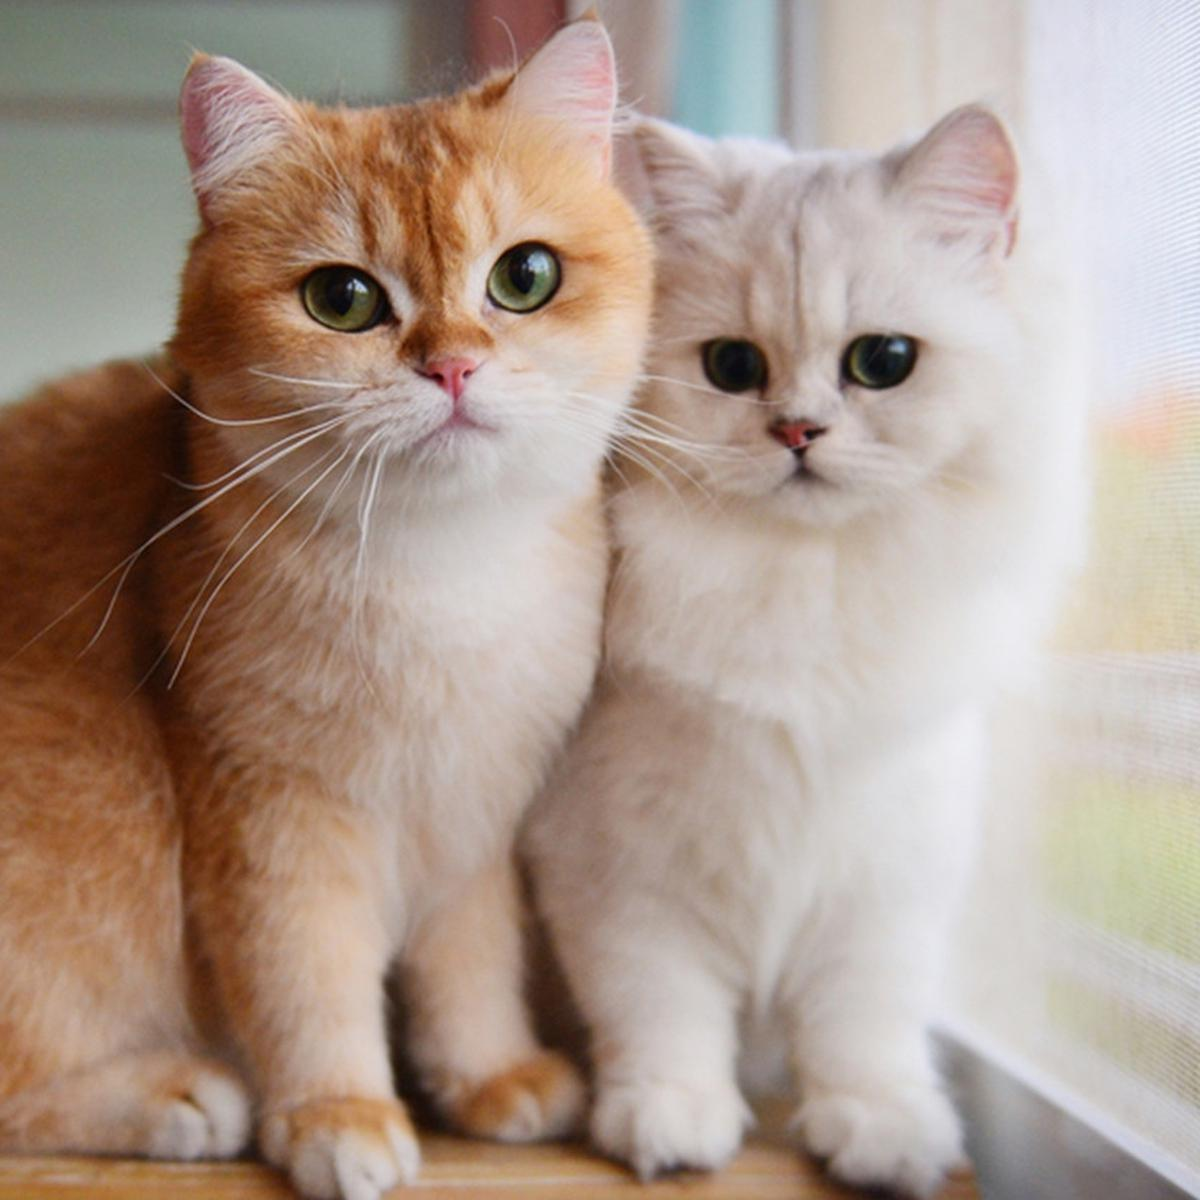
\includegraphics[scale=0.2]{gambar-kucing.jpg}
        \caption{Gambar Kucing Lucu dan Imut}
        \label{fig:kucing}
    \end{figure}
\end{lstlisting}

\noindent Berikut adalah penjelasan dari setiap baris pada kode di atas:

\begin{packed_enum}
    \item \texttt{\textbackslash begin\{figure\}[H] ... \textbackslash end\{figure\}}: Membuat lingkungan \texttt{figure} untuk menyisipkan gambar. Parameter \texttt{[H]} digunakan agar gambar diletakkan tepat di posisi yang ditentukan dalam kode. Opsi \textit{H} dapat diganti dengan \textit{h, t, b, p} sesuai kebutuhan.
    \item \texttt{\textbackslash centering}: Mengatur gambar agar berada di tengah halaman.
    \item \texttt{\textbackslash includegraphics[scale=0.2]\{gambar-kucing.jpg\}}: Memasukkan gambar dengan nama file \texttt{gambar-kucing.jpg}. Parameter \texttt{scale=0.2} mengatur ukuran gambar pada 20\% dari ukuran aslinya. Ubah nilainya untuk memperbesar atau memperkecil gambar.
    \item \texttt{\textbackslash caption\{Gambar Kucing Lucu dan Imut\}}: Menambahkan keterangan (caption) di bawah gambar yang akan muncul di Daftar Gambar dan disertai nomor gambar secara otomatis.
    \item \texttt{\textbackslash label\{fig:kucing\}}: Memberikan label pada gambar untuk merujuk gambar ini dalam teks menggunakan \texttt{\textbackslash cref\{fig:kucing\}} atau \texttt{\textbackslash ref\{fig:kucing\}} yang menghasilkan "Gambar 1" atau penomoran gambar sesuai urutan.
\end{packed_enum}

Hasilnya adalah terlihat seperti pada \cref{fig:kucing}.

\begin{figure}[H]
    \centering
    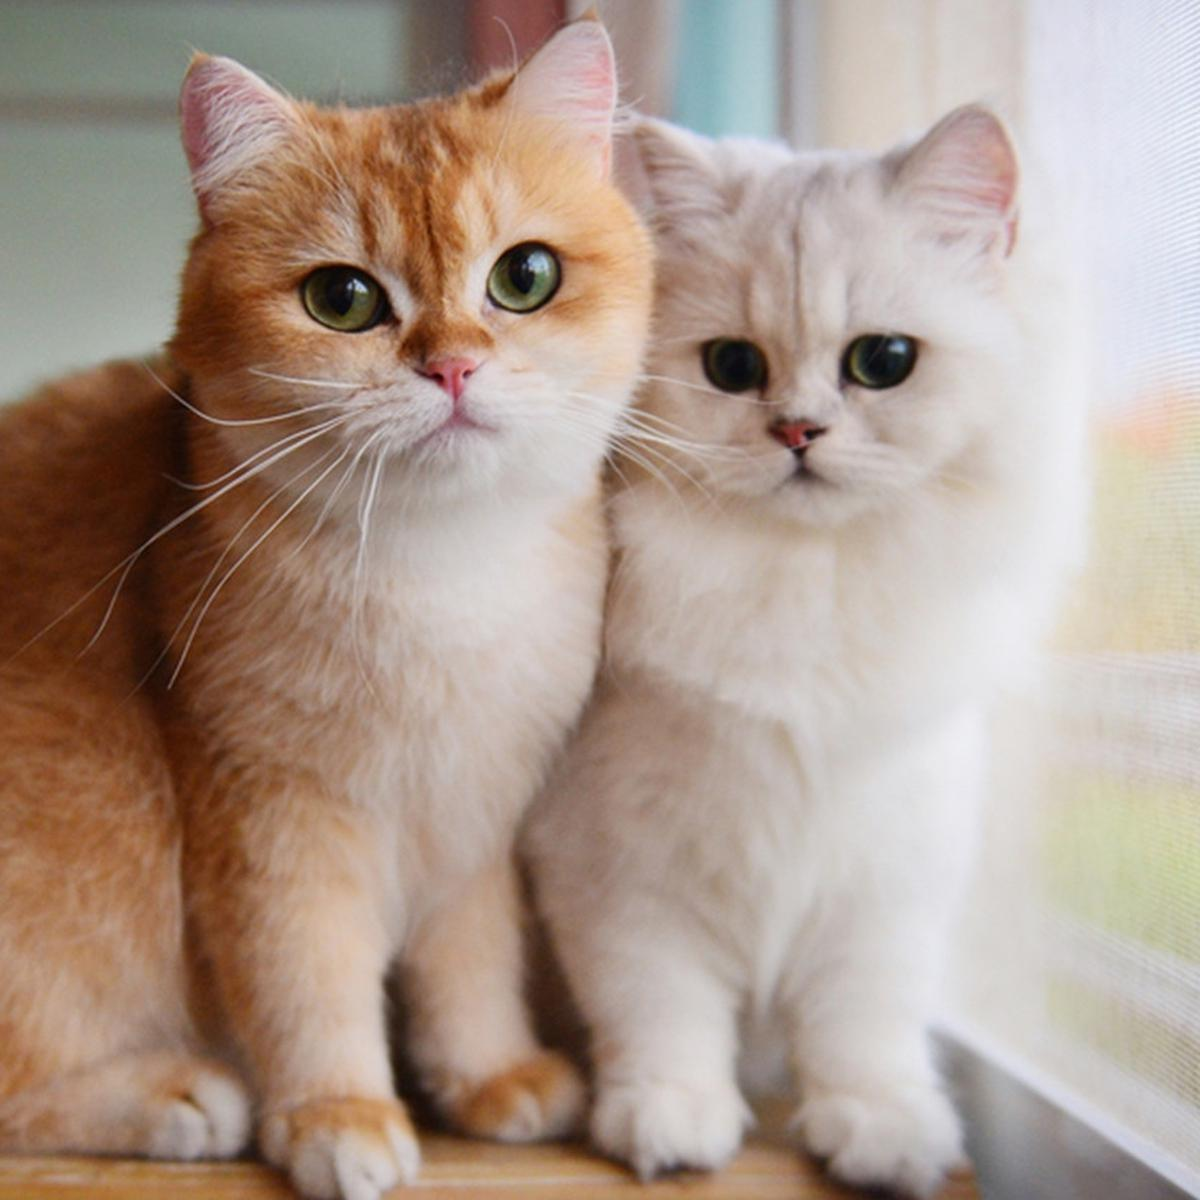
\includegraphics[scale=0.1]{gambar-kucing}
    \caption{Gambar Kucing Lucu dan Imut dengan scala 0.1}
    \label{fig:kucing}
\end{figure}

Setiap gambar harus dimention atau disebutkan didalam bacaan seperti berikut ini \cref{fig:kucing} dan \cref{fig:logoUBS}.

\begin{figure}[H]
    \centering
    
\includegraphics[scale=0.4]{logo-ubs}
    \caption{Logo UBS dengan scala 0.4}
    \label{fig:logoUBS}
\end{figure}

Untuk menyisipkan beberapa gambar dalam satu kelompok dan satu caption utama, kita dapat menggunakan lingkungan \texttt{subfigure} di dalam lingkungan \texttt{figure}. Metode ini sangat bermanfaat jika kita ingin menyusun beberapa gambar berukuran kecil dalam satu baris atau kolom, dengan setiap gambar diberi caption masing-masing dan satu caption utama untuk keseluruhan gambar.

Kode berikut menunjukkan cara menyusun tiga gambar secara berdampingan dengan satu caption utama.

\begin{lstlisting}[language=TeX, caption=Kode untuk Menyisipkan Gambar dalam Dokumen dengan Subfigure, label=lst:kode_gambar_multi]
    \begin{figure}
        \centering
        \begin{subfigure}[b]{0.3\textwidth}
            \centering
            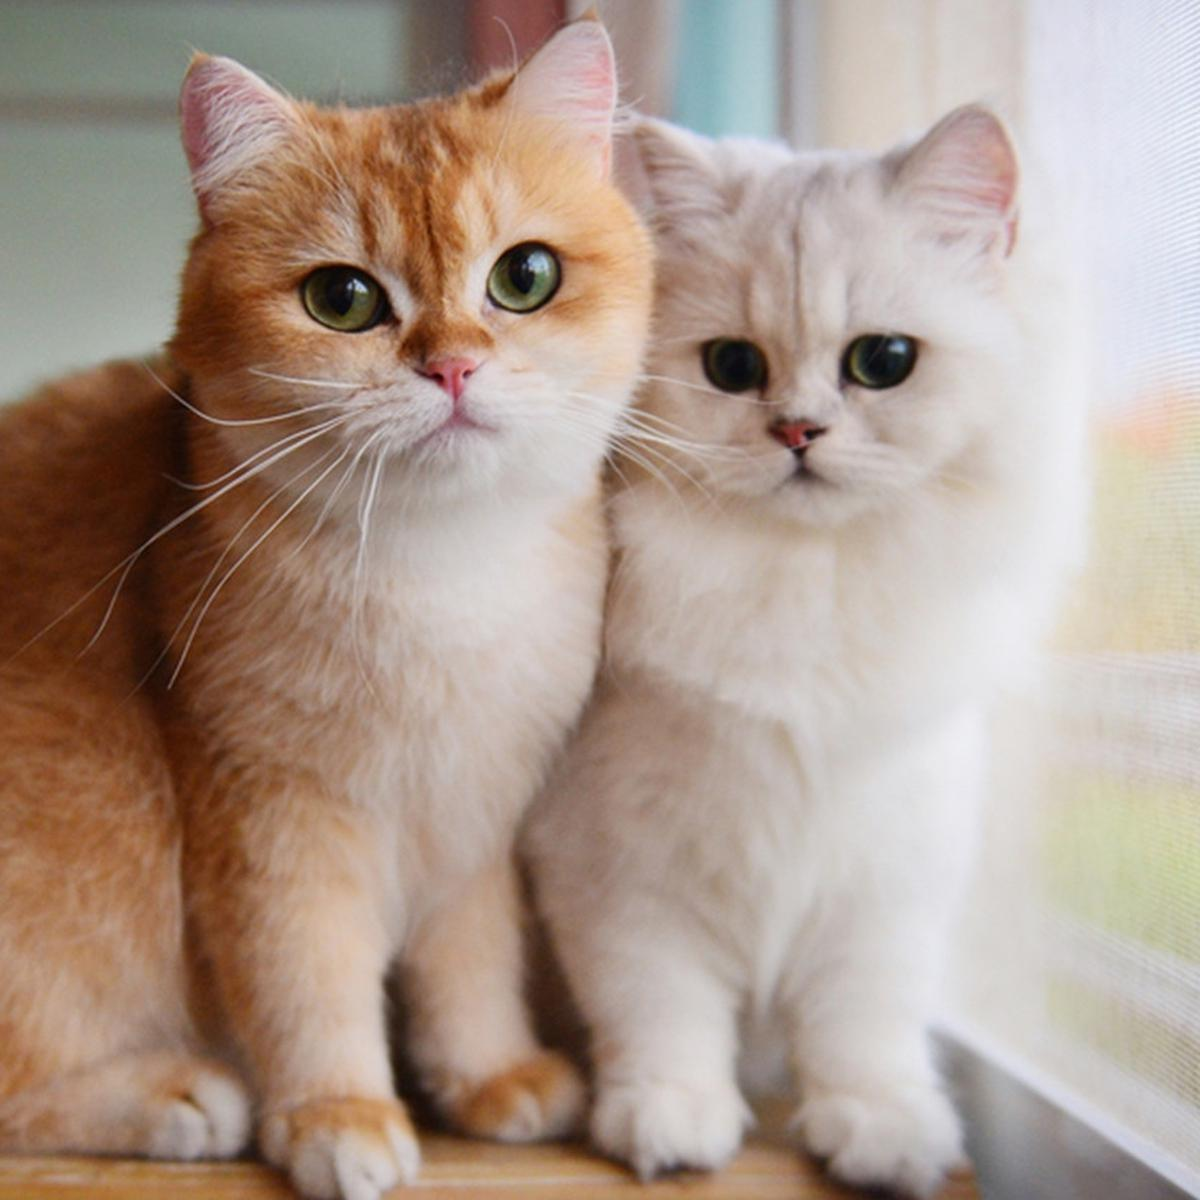
\includegraphics[width=\linewidth]{gambar-kucing.jpg}
            \caption{Kucing Lucu 1}
            \label{fig:kucing-a}
        \end{subfigure}
        \hfill
        \begin{subfigure}[b]{0.3\textwidth}
            \centering
            
\includegraphics[width=\linewidth]{logo-ubs.png}
            \caption{Logo UBS}
            \label{fig:logo-ubs-b}
        \end{subfigure}
        \hfill
        \begin{subfigure}[b]{0.3\textwidth}
            \centering
            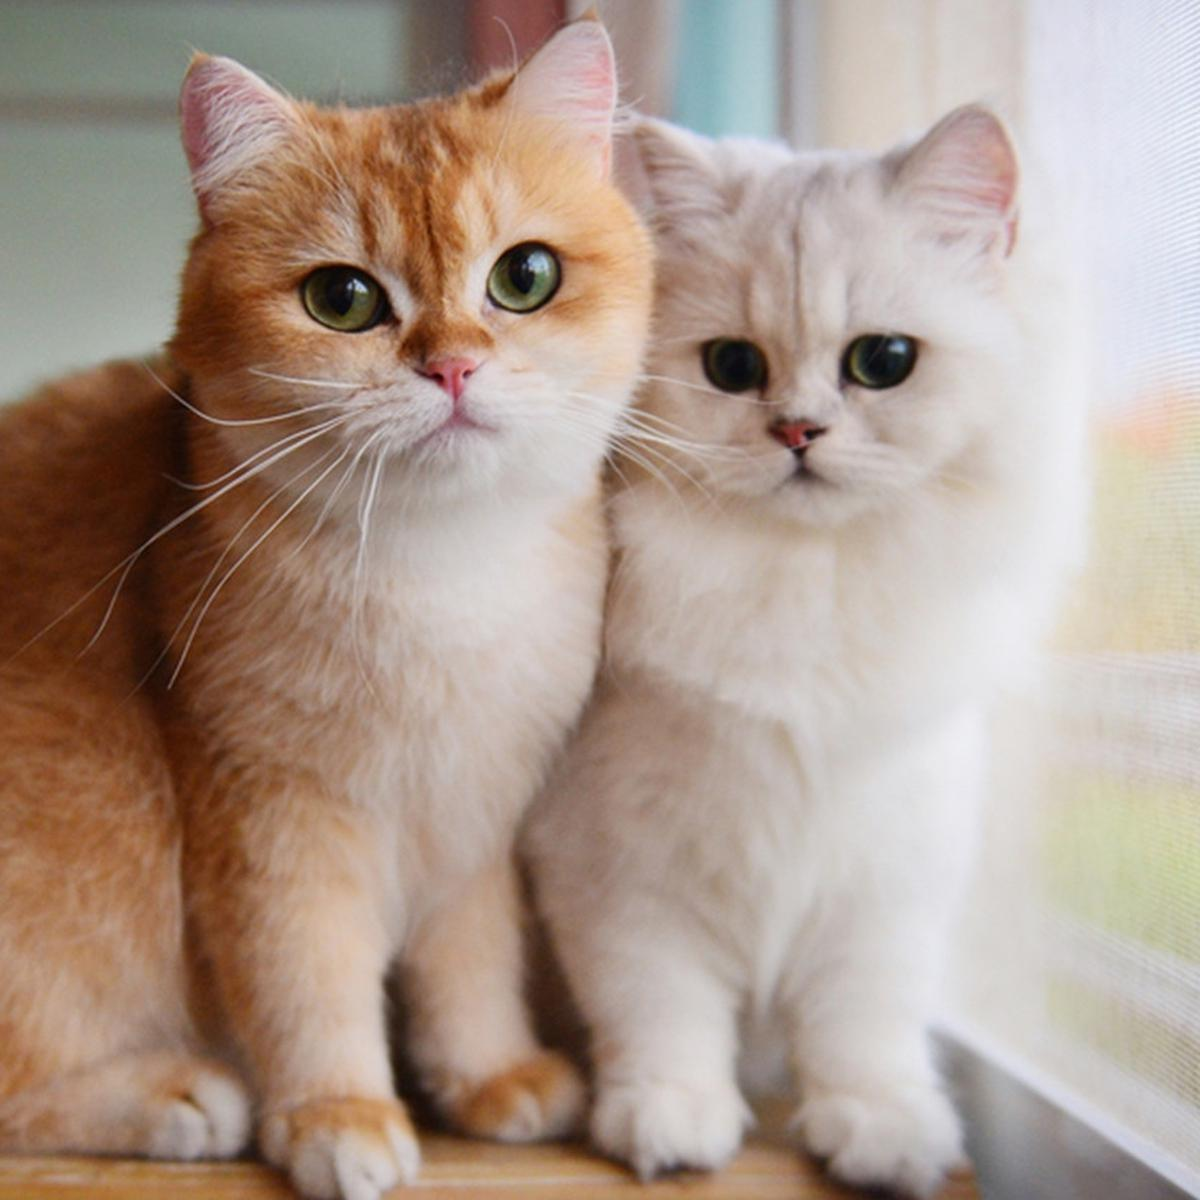
\includegraphics[width=\linewidth]{gambar-kucing.jpg}
            \caption{Kucing Lucu 2}
            \label{fig:kucing-c}
        \end{subfigure}
        \caption{Beberapa gambar yang disusun menjadi 1 bagian dengan penomoran (a), (b), dan (c)}
        \label{fig:kucingdanUBS}
    \end{figure}
\end{lstlisting}

\noindent Berikut adalah penjelasan dari setiap bagian kode di atas:

\begin{packed_enum}
    \item \texttt{\textbackslash begin\{figure\} ... \textbackslash end\{figure\}}: Lingkungan \texttt{figure} utama yang berfungsi sebagai wadah untuk menyisipkan beberapa gambar dalam satu bagian.
    
    \item \texttt{\textbackslash begin\{subfigure\}[b]\{0.3\textbackslash textwidth\} ... \textbackslash end\{subfigure\}}: Lingkungan \texttt{subfigure} digunakan untuk setiap gambar yang ingin disusun dalam satu bagian. Parameter \texttt{0.3\textbackslash textwidth} mengatur lebar setiap gambar menjadi sepertiga dari lebar teks, sehingga tiga gambar dapat ditampilkan berdampingan dalam satu baris.
    
    \item \texttt{\textbackslash includegraphics[width=\textbackslash linewidth]\{gambar-nama\}}: Memasukkan setiap gambar dengan lebar yang sesuai dengan lebar yang telah ditentukan untuk \texttt{subfigure}. 
        \begin{packed_enum}
            \item Gambar pertama menggunakan file \texttt{gambar-kucing}, dengan caption "Kucing Lucu 1".
            \item Gambar kedua menggunakan file \texttt{logo-ubs}, dengan caption "Logo UBS".
            \item Gambar ketiga juga menggunakan file \texttt{gambar-kucing}, dengan caption "Kucing Lucu 2".
        \end{packed_enum}
    
    \item \texttt{\textbackslash hfill}: Menyisipkan ruang kosong antar gambar, agar setiap \texttt{subfigure} memiliki jarak yang merata.
    
    \item \texttt{\textbackslash caption\{...\}}: Caption utama yang menjelaskan ketiga gambar sekaligus. Caption ini akan ditampilkan di bawah semua gambar dalam lingkungan \texttt{figure}.

    \item \texttt{\textbackslash label\{fig:kucingdanUBS\}}: Memberikan label untuk keseluruhan kelompok gambar, sehingga kita bisa merujuk ke seluruh bagian gambar ini dalam teks dengan \texttt{\textbackslash cref\{fig:kucingdanUBS\}}.
\end{packed_enum}

Dengan menggunakan metode ini, Anda dapat menyisipkan beberapa gambar dalam satu bagian dengan satu caption utama seperti pada \cref{fig:kucingdanUBS}. Setiap gambar dapat memiliki caption terpisah dan nomor (misalnya, (a), (b), (c)), sehingga rujukan spesifik untuk masing-masing gambar dapat dibuat, seperti \texttt{\textbackslash cref\{fig:kucing-a\}} untuk merujuk ke \cref{fig:kucing-a}.

\begin{figure}
    \centering
    \begin{subfigure}[b]{0.3\textwidth}
        \centering
        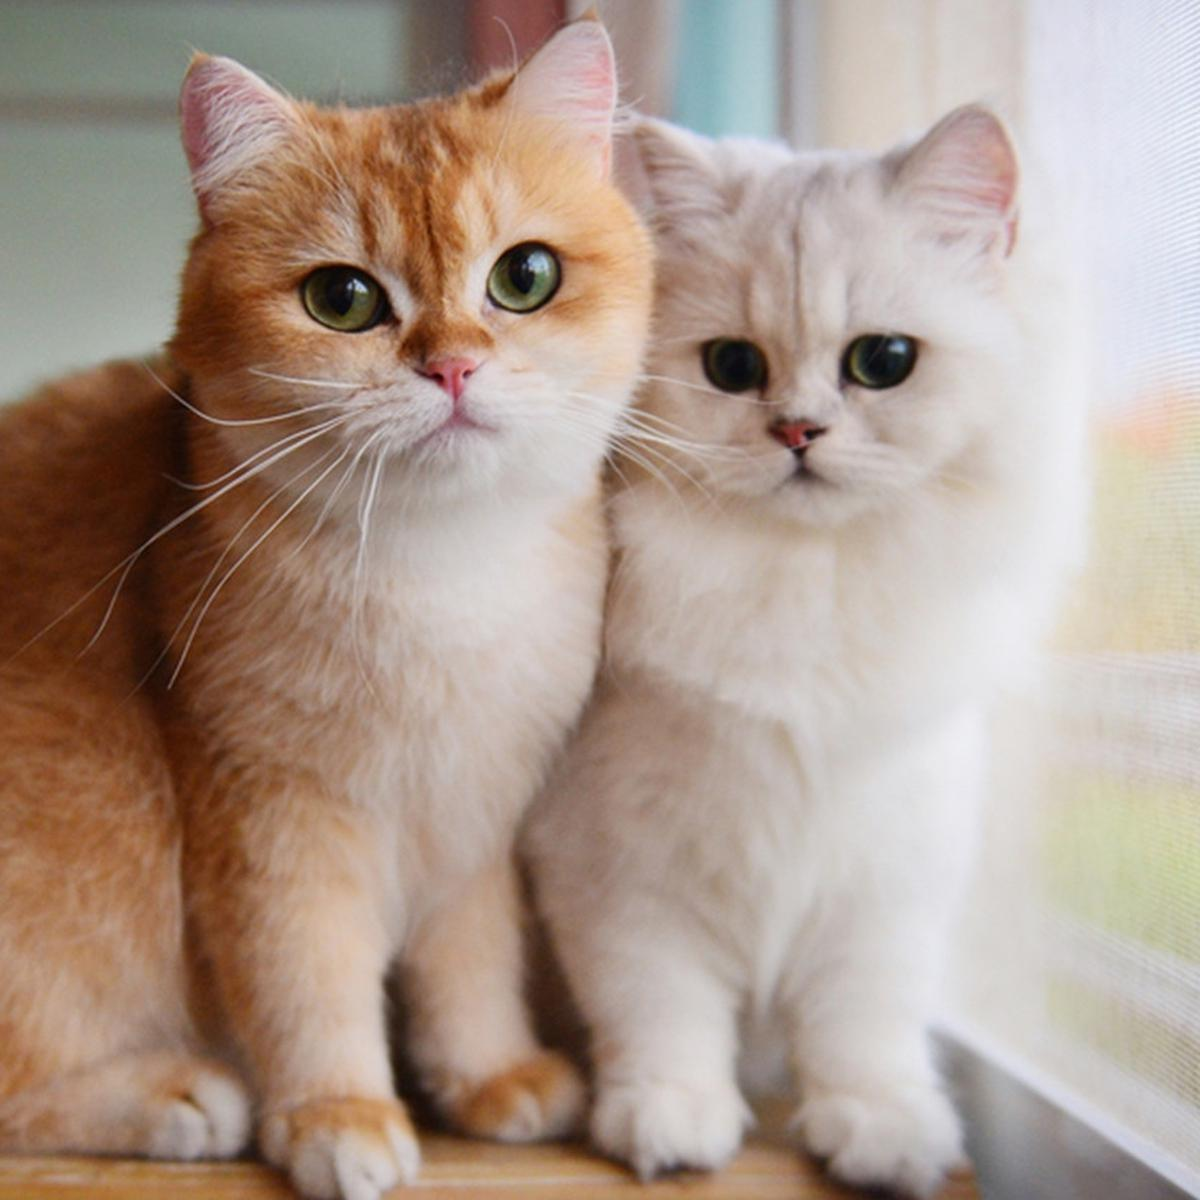
\includegraphics[width=\linewidth]{gambar-kucing.jpg}
        \caption{Kucing Lucu 1}
        \label{fig:kucing-a}
    \end{subfigure}
    \hfill
    \begin{subfigure}[b]{0.3\textwidth}
        \centering
        
\includegraphics[width=\linewidth]{logo-ubs.png}
        \caption{Logo UBS}
        \label{fig:logo-ubs-b}
    \end{subfigure}
    \hfill
    \begin{subfigure}[b]{0.3\textwidth}
        \centering
        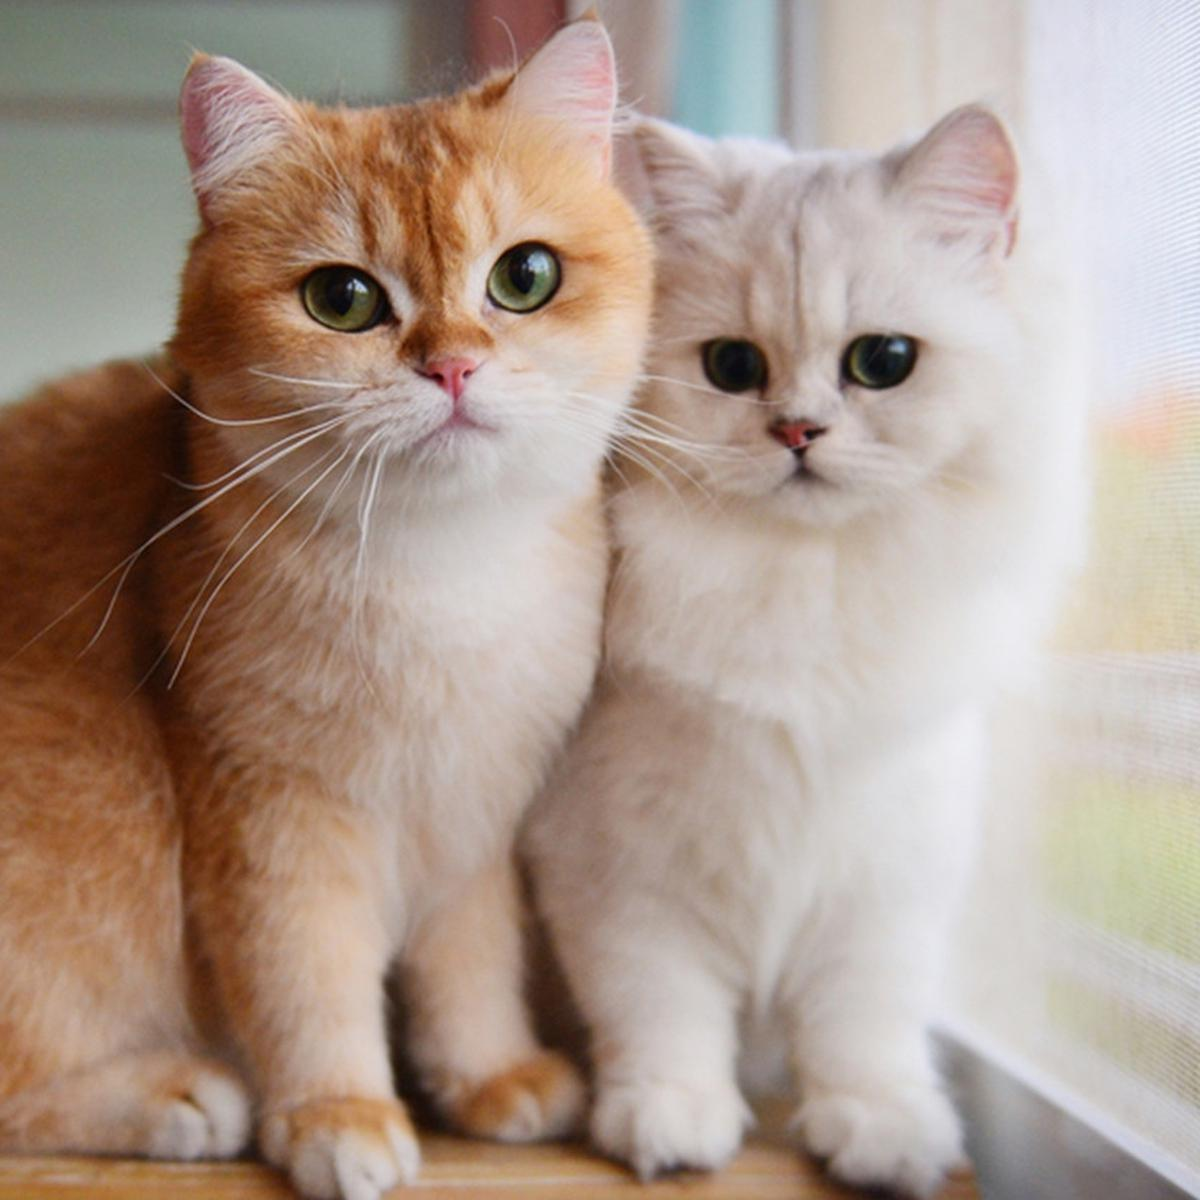
\includegraphics[width=\linewidth]{gambar-kucing.jpg}
        \caption{Kucing Lucu 2}
        \label{fig:kucing-c}
    \end{subfigure}
    \caption{Beberapa gambar yang disusun menjadi 1 bagian dengan penomoran (a), (b), dan (c)}
    \label{fig:kucingdanUBS}
\end{figure}

\section{Membuat Grafik dengan Tikz}
TikZ adalah sebuah paket LaTeX yang digunakan untuk membuat grafik vektor. Berikut adalah beberapa contoh dasar penggunaan TikZ.

\subsection{Menggambar Garis dan Bentuk Dasar}
Untuk menggambar garis dan bentuk dasar, kita bisa menggunakan perintah-perintah berikut:
\begin{lstlisting}[language=TeX, caption=Kode untuk Menggambar Garis dan Bentuk Dasar, label=lst:Menggambar Garis dan Bentuk Dasar]
    \begin{figure}[H]
        \centering
        \begin{tikzpicture}
            \draw (0,0) -- (2,0);
            \draw (0,0) rectangle (2,2);
            \draw (1,1) circle (1);
        \end{tikzpicture}
        \caption{Menggambar Garis dan Bentuk Dasar}
        \label{fig:tikzExample}
    \end{figure}
\end{lstlisting}

\begin{figure}[H]
    \centering
    \begin{tikzpicture}
        \draw (0,0) -- (2,0);
        \draw (0,0) rectangle (2,2);
        \draw (1,1) circle (1);
    \end{tikzpicture}
    \caption{Menggambar Garis dan Bentuk Dasar}
    \label{fig:tikzExample}
\end{figure}

Pada Gambar \ref{fig:tikzExample} dapat dilihat contoh gambar sederhana.

\subsection{Menggambar Grafik Fungsi}
TikZ juga bisa digunakan untuk menggambar grafik fungsi matematika:
\begin{lstlisting}[language=TeX, caption=Kode untuk Menggambar Grafik Fungsi, label=lst:Menggambar Grafik Fungsi]
    \begin{figure}[H]
        \centering
        \begin{tikzpicture}
            \begin{axis}[
                axis lines = middle,
                xlabel = $x$,
                ylabel = {$f(x)$},
                title = {Grafik Fungsi Kuadrat},
                grid = major,
                xmin = -10, 
                xmax = 10,
                ymin = 0, 
                ymax = 100
            ]
            \addplot [
                domain=-10:10, 
                samples=100, 
                color=blue,
            ]
            {x^2};
            \end{axis}
        \end{tikzpicture}
        \caption{Grafik fungsi \( f(x) = x^2 \) dengan domain \( [-10, 10] \)}
        \label{fig:grafik_kuadrat}
    \end{figure}
\end{lstlisting}

\begin{figure}[H]
    \centering
    \begin{tikzpicture}
        \begin{axis}[
            axis lines = middle,
            xlabel = $x$,
            ylabel = {$f(x)$},
            title = {Grafik Fungsi Kuadrat},
            grid = major,
            xmin = -10, 
            xmax = 10,
            ymin = 0, 
            ymax = 100
        ]
        \addplot [
            domain=-10:10, 
            samples=100, 
            color=blue,
        ]
        {x^2};
        \end{axis}
    \end{tikzpicture}
    \caption{Grafik fungsi \( f(x) = x^2 \) dengan domain \( [-10, 10] \)}
    \label{fig:grafik_kuadrat}
\end{figure}

Pada Gambar \ref{fig:grafik_kuadrat} ditunjukkan grafik fungsi kuadrat.

\subsection{Menggambar Diagram Alir}
TikZ juga mendukung pembuatan diagram alir (flowchart):
\begin{lstlisting}[language=TeX, caption=Kode untuk Menggambar Diagram Alir, label=lst:Menggambar Diagram Alir]
    \begin{figure}[H]
        \centering
        \begin{tikzpicture}[node distance=2cm]
            \node (start) [startstop] {Start};
            \node (process1) [process, below of=start] {Process 1};
            \node (decision) [decision, below of=process1] {Decision};
            \node (process2a) [process, below of=decision, yshift=-1cm] {Process 2a};
            \node (process2b) [process, right of=decision, xshift=2cm] {Process 2b};
            \node (stop) [startstop, below of=process2a] {Stop};
    
            \draw [arrow] (start) -- (process1);
            \draw [arrow] (process1) -- (decision);
            \draw [arrow] (decision) -- node[anchor=east] {yes} (process2a);
            \draw [arrow] (decision) -- node[anchor=south] {no} (process2b);
            \draw [arrow] (process2a) -- (stop);
        \end{tikzpicture}
        \caption{Diagram alir sederhana dengan kondisi percabangan}
        \label{fig:flowchart_sederhana}
    \end{figure}
\end{lstlisting}
\begin{figure}[H]
    \centering
    \begin{tikzpicture}[node distance=2cm]
        \node (start) [startstop] {Start};
        \node (process1) [process, below of=start] {Process 1};
        \node (decision) [decision, below of=process1] {Decision};
        \node (process2a) [process, below of=decision, yshift=-1cm] {Process 2a};
        \node (process2b) [process, right of=decision, xshift=2cm] {Process 2b};
        \node (stop) [startstop, below of=process2a] {Stop};

        \draw [arrow] (start) -- (process1);
        \draw [arrow] (process1) -- (decision);
        \draw [arrow] (decision) -- node[anchor=east] {yes} (process2a);
        \draw [arrow] (decision) -- node[anchor=south] {no} (process2b);
        \draw [arrow] (process2a) -- (stop);
    \end{tikzpicture}
    \caption{Diagram alir sederhana dengan kondisi percabangan}
    \label{fig:flowchart_sederhana}
\end{figure}
Pada Gambar \ref{fig:flowchart_sederhana} ditunjukkan contoh diagram alir sederhana dengan satu kondisi percabangan.

\subsection{Menggambar Grafik Batang}
Untuk menggambar grafik batang, kita bisa menggunakan perintah berikut:
\begin{lstlisting}[language=TeX, caption=Kode untuk Menggambar Grafik Batang, label=lst:Menggambar Grafik Batang]
    \begin{figure}[H]
        \centering
        \begin{tikzpicture}
            \begin{axis}[
                ybar,
                symbolic x coords={A, B, C, D},
                xtick=data,
                ylabel={Nilai},
                xlabel={Kategori},
                title={Grafik Batang Sederhana},
                bar width=0.5cm,
                ymin=0,
                ymajorgrids=true
            ]
            \addplot[fill=blue!50] coordinates {(A,1) (B,3) (C,2) (D,4)};
            \end{axis}
        \end{tikzpicture}
        \caption{Grafik batang yang menunjukkan nilai untuk kategori A, B, C, dan D}
        \label{fig:grafik_batang}
    \end{figure}
\end{lstlisting}
\begin{figure}[H]
    \centering
    \begin{tikzpicture}
        \begin{axis}[
            ybar,
            symbolic x coords={A, B, C, D},
            xtick=data,
            ylabel={Nilai},
            xlabel={Kategori},
            title={Grafik Batang Sederhana},
            bar width=0.5cm,
            ymin=0,
            ymajorgrids=true
        ]
        \addplot[fill=blue!50] coordinates {(A,1) (B,3) (C,2) (D,4)};
        \end{axis}
    \end{tikzpicture}
    \caption{Grafik batang yang menunjukkan nilai untuk kategori A, B, C, dan D}
    \label{fig:grafik_batang}
\end{figure}
Pada Gambar \ref{fig:grafik_batang} dapat dilihat distribusi nilai pada berbagai kategori.

\subsection{Menggambar Grafik Pie}
TikZ juga mendukung pembuatan grafik pie:
\begin{lstlisting}[language=TeX, caption=Kode untuk Menggambar Grafik Pie, label=lst:Menggambar Grafik Pie]
    \begin{figure}[H]
        \centering
        \begin{tikzpicture}
            \pie{30/A, 20/B, 50/C}
        \end{tikzpicture}
        \caption{Diagram lingkaran yang menunjukkan distribusi persentase A, B, dan C}
        \label{fig:pie_chart}
    \end{figure}
\end{lstlisting}
\begin{figure}[H]
    \centering
    \begin{tikzpicture}
        \pie{30/A, 20/B, 50/C}
    \end{tikzpicture}
    \caption{Diagram lingkaran yang menunjukkan distribusi persentase A, B, dan C}
    \label{fig:pie_chart}
\end{figure}
Pada Gambar \ref{fig:pie_chart} ditunjukkan pembagian persentase untuk kategori A, B, dan C.

Dengan contoh-contoh di atas, Anda dapat mulai membuat berbagai jenis grafik menggunakan TikZ di \LaTeX. Untuk informasi lebih lanjut, Anda dapat merujuk ke dokumentasi resmi TikZ.

\section{Membuat Tabel}
Pada bagian ini akan dijelaskan bagaimana membuat tabel dalam sebuah dokumen \LaTeX. untuk membuat tabel memang agak sedikit sulit, sehingga saya menyarankan menggunakan tool berikut \url{https://www.tablesgenerator.com/} atau \url{https://www.latex-tables.com/} kemudian isikan tabel pada tool generator tersebut dan salin kodenya ke dalam dokumen \LaTeX. Berikut adalah contoh dari sebuah tabel yang telah dibuat. Jangan lupa setiap tabel harus dimention dan dijelaskan dibacaan seperti berikut ini \cref{tab:hresult}. Contoh pembuatan tabel terlihat kodenya pada \cref{lst:kode_tabel}.

\begin{lstlisting}[language=TeX, caption=Kode untuk Membuat Tabel dalam Dokumen, label=lst:kode_tabel]
    \begin{table}[h]
        \caption{Performance Using Hard Decision Detection}
        \label{tab:hresult}
        \centering
        \begin{tabular}{c rrrrrrr}
            \hline\hline
            Audio Name&\multicolumn{7}{c}{Sum of Extracted Bits} \\ [0.5ex] 
            \hline
            Police & 5 & -1 & 5& 5& -7& -5& 3\\
            Midnight & 7 & -3 & 5& 3& -1& -3& 5\\
            News & 9 & -3 & 7& 9& -5& -1& 9\\[0.8ex]
            \hline
        \end{tabular}
    \end{table}
\end{lstlisting}

\noindent Berikut adalah penjelasan dari setiap bagian kode di atas:

\begin{packed_enum}
    \item \texttt{\textbackslash begin\{table\}[h] ... \textbackslash end\{table\}}: Lingkungan \texttt{table} digunakan untuk membuat tabel dan menempatkannya di posisi tertentu dalam dokumen. Parameter \texttt{[h]} menginstruksikan LaTeX untuk menempatkan tabel di posisi yang paling mendekati lokasi kode tersebut dalam teks. Jika posisi ini tidak berfungsi dengan baik, Anda bisa menggunakan parameter lain, seperti \texttt{[H]} (dari paket \texttt{float}) untuk menempatkan tabel di lokasi yang lebih spesifik.
    \item \texttt{\textbackslash caption\{Performance Using Hard Decision Detection\}}: Menambahkan keterangan (caption) di atas tabel. Caption ini akan otomatis ditampilkan dalam Daftar Tabel dan diberi nomor secara otomatis oleh LaTeX.
    \item \texttt{\textbackslash label\{tab:hresult\}}: Memberi label pada tabel, memungkinkan tabel dirujuk dalam teks menggunakan perintah \texttt{\textbackslash cref\{tab:hresult\}} atau \texttt{\textbackslash ref\{tab:hresult\}}, yang akan menghasilkan "Tabel 1" atau sesuai penomoran tabel.
    \item \texttt{\textbackslash centering}: Mengatur tabel agar berada di tengah halaman.
    \item \texttt{\textbackslash begin\{tabular\}\{c rrrrrrr\} ... \textbackslash end\{tabular\}}: Lingkungan \texttt{tabular} digunakan untuk membuat struktur tabel. Pengaturan kolom menggunakan karakter:
        \begin{packed_enum}
            \item \texttt{c}: Mengatur kolom pertama rata tengah.
            \item \texttt{r}: Mengatur tujuh kolom berikutnya rata kanan.
        \end{packed_enum}
    \item \texttt{\textbackslash hline}: Menambahkan garis horizontal di tabel. Dua \texttt{\textbackslash hline} berturut-turut digunakan untuk garis ganda pada bagian header tabel.
    \item \texttt{\textbackslash multicolumn\{7\}\{c\}\{Sum of Extracted Bits\}}: Menggabungkan tujuh kolom berikutnya menjadi satu sel besar yang berisi teks "Sum of Extracted Bits", yang disejajarkan ke tengah dengan pengaturan \texttt{c}.
    \item Isi tabel, seperti:
        \begin{packed_enum}
            \item \texttt{Police}: Data pada baris ini terkait audio "Police", dengan tujuh angka di kolom berikutnya yang merepresentasikan "Sum of Extracted Bits".
            \item Baris lain mengikuti format yang sama.
        \end{packed_enum}
    \item Jarak tambahan antara baris terakhir dan \texttt{\textbackslash hline} berikutnya diberikan dengan parameter opsional \texttt{[0.8ex]}, yang menambahkan spasi vertikal untuk keterbacaan.
\end{packed_enum}

Dengan penjelasan ini, kode menghasilkan tabel terstruktur yang diberi nomor secara otomatis dan dapat dirujuk di teks dokumen. Hasil tabel dari \cref{lst:kode_tabel} adalah terlihat pada \cref{tab:hresult}.

\begin{table}[h]
    \caption{Performance Using Hard Decision Detection}
    \label{tab:hresult}
    \centering
    \begin{tabular}{c rrrrrrr}
        \hline\hline
        Audio Name&\multicolumn{7}{c}{Sum of Extracted Bits} \\ [0.5ex] 
        \hline
        Police & 5 & -1 & 5& 5& -7& -5& 3\\
        Midnight & 7 & -3 & 5& 3& -1& -3& 5\\
        News & 9 & -3 & 7& 9& -5& -1& 9\\[0.8ex]
        \hline
    \end{tabular}
\end{table}

Kita juga bisa menambahkan tabel yang besar dengan format halaman landscape seperti contoh berikut dan mention tabel seperti berikut ini \cref{tab:LPer} dan berikut ini \cref{tab:PPer}.

\begin{lstlisting}[language=TeX, caption=Kode untuk Membuat Tabel dalam Dokumen dengan Sideway, label=lst:kode_tabel_sideway]
    \begin{sidewaystable}[htbp]
        \caption{Performance After Post Filtering}
        \label{tab:LPer}
        \centering
        \begin{tabular}{l c c rrrrrrr}
            \hline\hline
            Audio &Audibility & Decision &\multicolumn{7}{c}{Sum of Extracted Bits} 
            \\ [0.5ex] 
            \hline
            & &soft &1 & $-1$ & 1 & 1 & $-1$ & $-1$ & 1 \\[-1ex]
            \raisebox{1.5ex}{Police} & \raisebox{1.5ex}{5}&hard
            & 2 & $-4$ & 4 & 4 & $-2$ & $-4$ & 4 \\[1ex]
            & &soft & 1 & $-1$ & 1 & 1 & $-1$ & $-1$ & 1 \\[-1ex]
            \raisebox{1.5ex}{Beethoven} & \raisebox{1.5ex}{5}& hard
            &8 & $-8$ & 2 & 8 & $-8$ & $-8$ & 6 \\[1ex]
            & &soft & 1 & $-1$ & 1 & 1 & $-1$ & $-1$ & 1 \\[-1ex]
            \raisebox{1.5ex}{Metallica} & \raisebox{1.5ex}{5}& hard
            &4 & $-8$ & 8 & 4 & $-8$ & $-8$ & 8 \\[1ex]
            \hline
        \end{tabular}
    \end{sidewaystable}
\end{lstlisting}

\noindent Berikut adalah penjelasan dari setiap bagian kode di atas:

\begin{packed_enum}
    \item \texttt{\textbackslash begin\{sidewaystable\}[htbp] ... \textbackslash end\{sidewaystable\}}: Lingkungan \texttt{sidewaystable} dari paket \texttt{rotating} digunakan untuk menampilkan tabel dalam orientasi landscape. Parameter \texttt{[htbp]} menunjukkan preferensi posisi tabel pada dokumen. Pastikan Anda telah memuat paket \texttt{rotating} di preamble dengan perintah \texttt{\textbackslash usepackage\{rotating\}}.
    \item \texttt{\textbackslash caption\{Performance After Post Filtering\}}: Menambahkan caption (keterangan) di atas tabel. Caption ini akan otomatis dimasukkan dalam Daftar Tabel dan diberi nomor secara otomatis.
    \item \texttt{\textbackslash label\{tab:LPer\}}: Memberi label pada tabel, memungkinkan Anda merujuk tabel ini dalam teks menggunakan perintah \texttt{\textbackslash cref\{tab:LPer\}} atau \texttt{\textbackslash ref\{tab:LPer\}}, yang akan menghasilkan "Tabel 1" atau sesuai penomoran tabel.
    \item \texttt{\textbackslash centering}: Mengatur tabel agar berada di tengah halaman.
    \item \texttt{\textbackslash begin\{tabular\}\{l c c rrrrrrr\} ... \textbackslash end\{tabular\}}: Lingkungan \texttt{tabular} digunakan untuk membuat struktur tabel dengan pengaturan kolom sebagai berikut:
        \begin{packed_enum}
            \item \texttt{l}: Mengatur kolom pertama rata kiri untuk kolom "Audio".
            \item \texttt{c}: Mengatur kolom kedua dan ketiga rata tengah untuk kolom "Audibility" dan "Decision".
            \item \texttt{r}: Tujuh kolom berikutnya rata kanan untuk data "Sum of Extracted Bits".
        \end{packed_enum}
    \item \texttt{\textbackslash hline}: Menambahkan garis horizontal di tabel. Dua \texttt{\textbackslash hline} berturut-turut digunakan untuk garis ganda pada bagian header tabel.
    \item \texttt{\textbackslash multicolumn\{7\}\{c\}\{Sum of Extracted Bits\}}: Menggabungkan tujuh kolom berikutnya menjadi satu sel besar yang berisi teks "Sum of Extracted Bits", yang disejajarkan ke tengah dengan pengaturan \texttt{c}.
    \item Isi tabel, misalnya:
        \begin{packed_enum}
            \item Data pada baris pertama terkait audio "Police", dengan kolom audibility berisi nilai 5, dan data decision dengan dua opsi: "soft" dan "hard".
            \item Data "soft" pada baris pertama dan "hard" pada baris kedua diisi dengan angka sesuai kolom masing-masing.
            \item Untuk beberapa entri seperti "Police", "Beethoven", dan "Metallica", kolom audibility dan audio di tengah (seperti nilai 5) diangkat dengan perintah \texttt{\textbackslash raisebox} untuk memberikan efek centering pada teks.
        \end{packed_enum}
    \item \texttt{[1ex]} atau \texttt{[-1ex]}: Mengatur jarak antar baris untuk menjaga keterbacaan dan posisi elemen tabel yang lebih seimbang.
\end{packed_enum}

Kode ini akan menghasilkan tabel landscape dengan satu caption, beberapa kolom gabungan, dan penomoran otomatis dan hasilnya terlihat pada \cref{tab:LPer}.

\begin{sidewaystable}[htbp]
    \caption{Performance After Post Filtering}
    \label{tab:LPer}
    \centering
    \begin{tabular}{l c c rrrrrrr}
        \hline\hline
        Audio &Audibility & Decision &\multicolumn{7}{c}{Sum of Extracted Bits} 
        \\ [0.5ex] 
        \hline
        & &soft &1 & $-1$ & 1 & 1 & $-1$ & $-1$ & 1 \\[-1ex]
        \raisebox{1.5ex}{Police} & \raisebox{1.5ex}{5}&hard
        & 2 & $-4$ & 4 & 4 & $-2$ & $-4$ & 4 \\[1ex]
        & &soft & 1 & $-1$ & 1 & 1 & $-1$ & $-1$ & 1 \\[-1ex]
        \raisebox{1.5ex}{Beethoven} & \raisebox{1.5ex}{5}& hard
        &8 & $-8$ & 2 & 8 & $-8$ & $-8$ & 6 \\[1ex]
        & &soft & 1 & $-1$ & 1 & 1 & $-1$ & $-1$ & 1 \\[-1ex]
        \raisebox{1.5ex}{Metallica} & \raisebox{1.5ex}{5}& hard
        &4 & $-8$ & 8 & 4 & $-8$ & $-8$ & 8 \\[1ex]
        \hline
    \end{tabular}
\end{sidewaystable}

Contoh lain \cref{lst:kode_tabel_lain} untuk pembuatan tabel seperti di bawah ini dan hasilnya tertampil pada \cref{tab:PPer}.

\begin{lstlisting}[language=TeX, caption=Kode untuk Membuat Tabel dalam Dokumen, label=lst:kode_tabel_lain]
    \begin{table}[ht]
        \caption{Performance After Post Filtering}
        \label{tab:PPer}
        \centering
        \begin{tabular}{l c c rrrrrrr}
            \hline\hline
            Audio &Audibility & Decision &\multicolumn{7}{c}{Sum of Extracted Bits} 
            \\ [0.5ex] 
            \hline
            & &soft &1 & $-1$ & 1 & 1 & $-1$ & $-1$ & 1 \\[-1ex]
            \raisebox{1.5ex}{Police} & \raisebox{1.5ex}{5}&hard
            & 2 & $-4$ & 4 & 4 & $-2$ & $-4$ & 4 \\[1ex]
            & &soft & 1 & $-1$ & 1 & 1 & $-1$ & $-1$ & 1 \\[-1ex]
            \raisebox{1.5ex}{Beethoven} & \raisebox{1.5ex}{5}& hard
            &8 & $-8$ & 2 & 8 & $-8$ & $-8$ & 6 \\[1ex]
            & &soft & 1 & $-1$ & 1 & 1 & $-1$ & $-1$ & 1 \\[-1ex]
            \raisebox{1.5ex}{Metallica} & \raisebox{1.5ex}{5}& hard
            &4 & $-8$ & 8 & 4 & $-8$ & $-8$ & 8 \\[1ex]
            \hline
        \end{tabular}
    \end{table}
\end{lstlisting}

\begin{table}[ht]
	\caption{Performance After Post Filtering}
	\label{tab:PPer}
	\centering
	\begin{tabular}{l c c rrrrrrr}
		\hline\hline
		Audio &Audibility & Decision &\multicolumn{7}{c}{Sum of Extracted Bits} 
		\\ [0.5ex] 
		\hline
		& &soft &1 & $-1$ & 1 & 1 & $-1$ & $-1$ & 1 \\[-1ex]
		\raisebox{1.5ex}{Police} & \raisebox{1.5ex}{5}&hard
		& 2 & $-4$ & 4 & 4 & $-2$ & $-4$ & 4 \\[1ex]
		& &soft & 1 & $-1$ & 1 & 1 & $-1$ & $-1$ & 1 \\[-1ex]
		\raisebox{1.5ex}{Beethoven} & \raisebox{1.5ex}{5}& hard
		&8 & $-8$ & 2 & 8 & $-8$ & $-8$ & 6 \\[1ex]
		& &soft & 1 & $-1$ & 1 & 1 & $-1$ & $-1$ & 1 \\[-1ex]
		\raisebox{1.5ex}{Metallica} & \raisebox{1.5ex}{5}& hard
		&4 & $-8$ & 8 & 4 & $-8$ & $-8$ & 8 \\[1ex]
		\hline
	\end{tabular}
\end{table}

\section{Menambahkan Persamaan}

Persamaan tidak lepas dari bidang ilmu teknik dan kadang perlu dituliskan dalam sebuah laporan. Sangat mudah menuliskan persamaan pada sebuah dokumen \LaTeX. Terdapat 2 jenis penulisan persamaan, yaitu inline dengan text seperti contoh ini \(x^2 + y^2 = z^2\) atau seperti ini $E=mc^2$. Jenis lain adalah dituliskan seperti di bawah ini, yang otomatis akan mendapatkan penomoran. Apabila belum familiar dengan kode untuk penulisan persamaan pada \LaTeX, Anda bisa menggunakan tool berikut \url{https://latex.codecogs.com/eqneditor/editor.php} atau \url{https://latexeditor.lagrida.com/}. Setiap persamaan harus disebutkan dalam teks seperti \cref{eq:satu} dan \cref{eq:equationDua} dan dijelaskan terkait persamaan tersebut untuk apa.

\begin{lstlisting}[language=TeX, caption=Kode untuk Menulis Persamaan, label=lst:kode_persamaan_emc]
    \begin{equation}
        \label{eq:satu}
        E=mc^2
    \end{equation}
\end{lstlisting}

\begin{lstlisting}[language=TeX, caption=Kode untuk Menulis Persamaan, label=lst:kode_persamaan_mn]
    \begin{equation}
        \label{eq:equationDua}
        m_n = k_p*e_n + \frac{k_e*T}{T_{reset}}\sum_{i=0}^{n}e_i + k_d\frac{e_n - e_{n-1}}{\delta t} + m_{R}
    \end{equation}
\end{lstlisting}

\noindent Berikut adalah penjelasan dari setiap bagian kode di atas:

Dengan menggunakan lingkungan \texttt{equation}, Anda bisa menulis dan memberi nomor persamaan secara otomatis serta merujuknya dengan mudah dalam teks menggunakan \texttt{\textbackslash cref}.

\begin{equation}
    \label{eq:satu}
    E=mc^2
\end{equation}

\begin{equation}
    \label{eq:equationDua}
    m_n = k_p*e_n + \frac{k_e*T}{T_{reset}}\sum_{i=0}^{n}e_i + k_d\frac{e_n - e_{n-1}}{\delta t} + m_{R}
\end{equation}

\section{Referensi dan Sitasi}
Referensi dan sitasi pada dokumen \LaTeX juga cukup mudah. Silahkan buka file \textit{pustaka.bib} dan amati beberapa contoh penulisan referensi yang ada. Untuk menggenerate bentuk referensi seperti ini dapat menggunakan Mendeley atau Zotero. Mensitasi referensi seperti ini \citep{Priambodo_2021}, \citep{Nasuha_2017}, \citep{Dhewa_Dharmawan_Priyambodo_2017}, \citep{Arifin_2015} dapat dilakukan dengan perintah \verb|\citep{nama_label}|. Pemberian sitasi dengan benar membuat sitasi tersebut dapat di klik dan akan mengarahkan ke daftar pustaka. %HANYA TUTORIAL. HAPUS SAAT PENULISAN
	\end{spacing}
}{

	%==================================================================
% Ini adalah sampul luar
%==================================================================

%% DILARANG EDIT BAGIAN INI

\begin{titlepage}
    \begin{center}

        \begin{doublespace}
            \textbf{\Large{\MakeUppercase{\judulid}}}\\[2cm]
        \end{doublespace}
        \textbf{\MakeUppercase{\large{\tipe}}}\\[0.5cm]

        Diajukan Sebagai Salah Satu Syarat Untuk Memperoleh Gelar Sarjana Terapan Pada Program Studi Teknik Elektronika {\fakultas} {\universitas}\\[1.5cm]

        \includegraphics[width=0.3\linewidth]{gambar/logo-uny.png}\\[1.5cm]

        \textbf{Oleh:} \\
        \textbf{\MakeUppercase{{\penulis}}} \\
        \textbf{NIM} \textbf{{\nim}}\\[2cm]

        \vfill

        \textbf{\large \MakeUppercase{Prodi \prodi}}\\
        \textbf{\large \MakeUppercase{\fakultas}}\\
        \textbf{\large \MakeUppercase{\universitas}}\\
        \textbf{\large \the\year{}}\\
    \end{center}
\end{titlepage}

%% DILARANG EDIT BAGIAN INI
	\pagenumbering{roman}
	%==================================================================
% Ini adalah sampul dalam
%==================================================================

%% DILARANG EDIT BAGIAN INI
\newpage
\addcontentsline{toc}{chapter}{HALAMAN SAMPUL}
\begin{center}
    \begin{doublespace}
        \textbf{\large{\MakeUppercase{\judulid}}}\\[2.5cm]
    \end{doublespace}

    \textbf{\MakeUppercase{\large{\tipe}}}\\[0.5cm]
    \begin{onehalfspace}
        Diajukan kepada {\fakultas} {\universitas} Untuk Memenuhi Sebagai Persyaratan Guna Memperoleh Gelar Sarjana Terapan\\[1.8cm]
    \end{onehalfspace}

    \large Oleh: \\
    \begin{onehalfspace}
        \large{\penulis} \\
        \large{\nim}\\[1.5cm]
    \end{onehalfspace}
    \vspace{1.5cm}

    \large Pembimbing: \\
    \begin{onehalfspace}
        \large{\pembimbing} \\
    \end{onehalfspace}

    \vfill

    \textbf{\large \MakeUppercase{Prodi \prodi}}\\
    \textbf{\large \MakeUppercase{\fakultas}}\\
    \textbf{\large \MakeUppercase{\universitas}}\\
    \textbf{\large \the\year{}}\\
\end{center}
%% DILARANG EDIT BAGIAN INI

	\begin{spacing}{1.2}
		%==================================================================
% Ini adalah abstrak dalam bahasa indonesia 
%==================================================================

%% DILARANG EDIT BAGIAN INI
\clearpage
\phantomsection
\addcontentsline{toc}{chapter}{ABSTRAK}
\noindent\textbf{\penulis, \nim}\\
\textbf{\MakeUppercase{\judulid}; dibimbing oleh {\pembimbingutama} dan {\pembimbingpendamping}.}\\
% \textbf{Hal.}
\textbf{\pageref{LastPage} + \getromanpagelast\ hal / \total{table} tabel / \total{figure} gambar / \total{lampiran} lampiran / \total{pustaka} pustaka (\tahunakademik)}
\begin{center}
    \textbf{ABSTRAK}\\[0.5cm]
\end{center}
%% DILARANG EDIT BAGIAN INI

%% edit bagian ini
Abstrak adalah sebuah ringkasan singkat yang menjelaskan secara umum tentang isi dari laporan tugas akhir. Abstrak ditulis dalam tiga (3) paragraf yang berisi beberapa kalimat yang menyatakan tujuan, metode, hasil, dan kesimpulan dari laporan tugas akhir. Paragraf pertama berisi latar belakang dan tujuan tugas akhir. Paragraf kedua berisi metode dan pembahasannya. Paragraf ketiga berisi hasil dan simpulan dari tugas akhir yang dikerjakan.

Abstrak harus menjelaskan secara jelas dan singkat apa yang dibahas dalam laporan tugas akhir, mengapa penelitian ini penting dan apa yang ditemukan dari penelitian tersebut. Abstrak harus ditulis dengan bahasa yang mudah dipahami dan harus mencakup informasi penting yang dibahas dalam laporan tugas akhir. 

Abstrak harus mengandung kata-kata yang relevan dengan laporan tugas akhir dan ditulis dengan bahasa yang formal dan akademik. Abstrak merupakan bagian penting dari sebuah laporan tugas akhir karena merupakan bagian yang pertama kali dibaca oleh pembaca dan harus dapat memberikan gambaran yang jelas tentang isi dari laporan tugas akhir. Oleh karena itu, abstrak harus ditulis dengan baik dan sebaik mungkin agar dapat memberikan gambaran yang jelas tentang laporan tugas akhir yang ditulis. Panjang abstrak sebaiknya dicukupkan dalam satu halaman, termasuk kata kunci. Tiga kata kunci dipandang cukup, yang masing-masingnya memuat paduan kata utama, yang dapat merepresentasikan isi Abstrak.\\[0.6cm]
%% edit sampai sini

%% DILARANG EDIT BAGIAN INI
\noindent Kata kunci: Konsep Abstrak, Komponen Abstrak, Kata Kunci.
%% DILARANG EDIT BAGIAN INI
		%==================================================================
% Ini adalah abstrak dalam bahasa inggris 
%==================================================================

%% DILARANG EDIT BAGIAN INI
\clearpage
\phantomsection
% \addcontentsline{toc}{chapter}{ABSTRACT}
\begin{center}
    % \textbf{\large{\judulen}}\\[0.5cm]
    % by:\\
    % \penulis\\
    % NIM: \nim\\[2em]
    \textbf{\textit{ABSTRACT}}\\[0.5cm]
\end{center}
%% DILARANG EDIT BAGIAN INI

%% edit bagian ini
\textit{The abstract is a short summary that explains in general the contents of the final assignment report. The abstract is written in three (3) paragraphs containing several sentences stating the objectives, methods, results and conclusions of the final assignment report. The first paragraph contains the background and objectives of the final assignment. The second paragraph contains the method and discussion. The third paragraph contains the results and conclusions of the final assignment carried out.}

\textit{The abstract must explain clearly and concisely what is discussed in the final project report, why this research is important and what was found from the research. The abstract must be written in language that is easy to understand and must include important information discussed in the final project report.}

\textit{The abstract must contain words that are relevant to the final project report and be written in formal and academic language. The abstract is an important part of a final assignment report because it is the part that is first read by the reader and must be able to provide a clear picture of the contents of the final assignment report. Therefore, the abstract must be written well and as well as possible in order to provide a clear picture of the final project report being written. The length of the abstract should be limited to one page, including keywords. Three keywords are considered sufficient, each of which contains a combination of main words, which can represent the contents of the Abstract.}\\[0.6cm]
%% edit sampai sini

%% DILARANG EDIT BAGIAN INI
\noindent\textit{Key words: Abstract Concepts, Abstract Components, Key Words.}
%% DILARANG EDIT BAGIAN INI
	\end{spacing}

	\begin{spacing}{1.5}
		%==================================================================
% Ini adalah lembar pernyataan
%==================================================================

%% Edit sesuai kebutuhan
\newpage
\addcontentsline{toc}{chapter}{LEMBAR PERNYATAAN KEASLIAN SKRIPSI}
\begin{center}
    \begin{doublespace}
        \textbf{\large \MakeUppercase{lembar pernyataan keaslian skripsi}}
    \end{doublespace}
\end{center}

\vspace{-\baselineskip}

\begin{table}[h!]
    \begin{tabular}{llp{3.5in}}    
        Nama              & : & \penulis \\[5pt]
        NIM               & : & \nim     \\[5pt]
        Program Studi     & : & \prodi   \\[5pt]
        Judul {\tipe}     & : & \MakeUppercase{\RaggedRight\judulid} \\
    \end{tabular}
\end{table}

Dengan ini saya menyatakan bahwa dalam skripsi ini tidak terdapat karya yang pernah diajukan untuk memperoleh gelar kesarjanaan di suatu Perguruan Tinggi, dan sepanjang pengetahuan saya juga tidak terdapat karya atau pendapat yang pernah ditulis atau diterbitkan oleh orang lain, kecuali yang secara tertulis dirujuk dalam naskah ini dan disebutkan dalam daftar pustaka.

Apabila dikemudian hari saya terbukti memberikan pernyataan yang tidak benar, saya bersedia menerima sanksi berupa pencabutan gelar kesarjanaan saya.

\vspace{2cm}

\begin{flushright}
    {\kota}, \textbf{\tglpernyataan}\\[3cm]
    \penulis \\
\end{flushright}

%% Edit sesuai kebutuhan
	\end{spacing}

	%==================================================================
% Ini adalah halaman persetujuan
%==================================================================

%% DILARANG EDIT BAGIAN INI
\newpage
\addcontentsline{toc}{chapter}{LEMBAR PERSETUJUAN UJIAN}
\begin{center}
    \begin{doublespace}
        \textbf{\large \MakeUppercase{lembar persetujuan}}
    \end{doublespace}
\end{center}

\begin{center}
    {\tipe} dengan Judul
\end{center}

\begin{center}
    \begin{doublespace}
        \textbf{\large \MakeUppercase {\judulid}}
    \end{doublespace}
\end{center}

\begin{center}
    Disusun oleh:\\
    \textbf{\penulis}\\
    \textbf{NIM \nim}\\[1.5cm]

    telah memenuhi syarat dan disetujui oleh Dosen Pembimbing untuk dilaksanakan Ujian {\tipe} bagi yang bersangkutan.\\[0.75cm]
\end{center}

\begin{minipage}{0.35\textwidth}
    \hfill\\[2em]
    Mengetahui,\\
    Koordinator Program Studi,\\[2cm]
    \resizebox{\textwidth}{!}{\koorprodi}\\
    NIP. \NIPkoorprodi
\end{minipage}
\hfill
\begin{minipage}{0.47\textwidth}
    Wates, \tglpersetujuan\\[1em]
    Disetujui,\\
    Dosen Pembimbing TA,\\[2cm]
    \resizebox{\textwidth}{!}{\pembimbing}\\
    NIP. \NIPpembimbing
\end{minipage}%
%% DILARANG EDIT BAGIAN INI
	%==================================================================
% Ini adalah lembar pengesahan
%==================================================================

%% DILARANG EDIT BAGIAN INI
\newpage
\addcontentsline{toc}{chapter}{LEMBAR PENGESAHAN \MakeUppercase{{\tipe}}}
\begin{center}
    \textbf{\large \MakeUppercase{lembar pengesahan {\tipe}}}
\end{center}

\begin{doublespace}
    \noindent{Telah disidangkan dan dinyatakan Lulus Sidang Skripsi pada Program {\gelar} ({\gelarsingkat}), Program Studi {\prodi} {\fakultas} {\universitas} pada \textbf{\tglpersetujuan} skripsi dengan judul:}
\end{doublespace}

\vspace{\baselineskip}

\begin{center}
    \begin{doublespace}
        \textbf{\MakeUppercase {\judulid}}
    \end{doublespace}
\end{center}

\vspace{-\baselineskip}

\begin{table}[h!]
    \centering
    \begin{tabular}{p{8cm}c}
        \multicolumn{1}{c}{Nama Penguji} & Tanda Tangan \\ 
        & \\ 
        & \\ 
        & \\ 
        \pengujisatu & \underline{\hspace{5cm}}\\ 
        NIDN: {\NIDNpengujisatu} & \\ 
        & \\ 
        & \\ 
        & \\ 
        \pengujidua & \underline{\hspace{5cm}}\\ 
        NIDN: {\NIDNpengujidua} & \\ 
        & \\ 
        & \\ 
        & \\ 
        \pengujitiga & \underline{\hspace{5cm}}\\ 
        NIDN: {\NIDNpengujitiga} &
    \end{tabular}
\end{table}

\vspace{\baselineskip}

\begin{center}
    \begin{doublespace}
        Mengetahui:\\
        Ketua Program Studi {\prodi}\\[3cm]
    \end{doublespace}
    ({\kaprodi})\\
\end{center}
%% DILARANG EDIT BAGIAN INI

	\begin{spacing}{1.2}
		%==================================================================
% Ini adalah halaman persembahan
%==================================================================

%% DILARANG EDIT BAGIAN INI
\clearpage
\phantomsection
\addcontentsline{toc}{chapter}{HALAMAN PERSEMBAHAN}
\begin{center}
    \textbf{\large HALAMAN PERSEMBAHAN}\\[3em]
\end{center}
%% DILARANG EDIT BAGIAN INI

%% Edit bagian ini sesuai kebutuhan

\begin{center}
    “Tugas Akhir ini saya persembahkan sepenuhnya kepada dua orang hebat dalam hidup saya, Ayahanda dan Ibunda. Keduanya lah yang membuat segalanya menjadi mungkin sehingga saya bisa sampai pada tahap di mana skripsi ini akhirnya selesai. Terima kasih atas segala pengorbanan, nasihat dan doa baik yang tidak pernah berhenti kalian berikan kepadaku. Aku selamanya bersyukur dengan keberadaan kalian sebagai orangtua ku.”
\end{center}

%% Edit bagian ini sesuai kebutuhan
		%==================================================================
% Ini adalah kata pengantar
%==================================================================

%% DILARANG EDIT BAGIAN INI
\clearpage
\phantomsection
\addcontentsline{toc}{chapter}{KATA PENGANTAR}
\begin{center}
    \textbf{\large KATA PENGANTAR}\\[3em]
\end{center}
%% DILARANG EDIT BAGIAN INI

%% Edit bagian ini sesuai kebutuhan
Dengan memanjatkan puji syukur kehadiran Allah SWT yang telah melimpahkan segala rahmat dan hidayahnya kepada Penulis, sehingga tersusunlah Skripsi yang berjudul "\textbf{\judulid}"

Skripsi ini merupakan salah satu persyaratan yang diajukan dalam rangka menempuh ujian akhir untuk memperoleh gelar {\gelar} {\gelarsingkat} pada Program Studi {\prodi}, Program Studi {\prodi} di {\fakultas} {\universitas}.

Penulis sungguh sangat menyadari, bahwa penulisan Skripsi ini tidak akan terwujud tanpa adanya dukungan dan bantuan dari berbagai pihak terutama Ayahanda dan Ibunda serta yang lainnya. Maka, dalam kesempatan ini penulis menghaturkan penghargaan dan ucapan terima kasih yang sebesar-besarnya kepada :

\begin{enumerate}
    \item {\pembimbingutama} selaku Dosen Pembimbing TA yang telah banyak memberikan semangat, dorongan, dan bimbingan selama penyusunan Tugas Akhir ini.
    \item {\pembimbingutama}, {\sekretaris}, {\penguji} selaku Ketua Penguji, Sekretaris, dan Penguji yang sudah  memberikan koreksi perbaikan secara komprehensif terhadap TA ini.
    \item {\koorprodi} selaku Ketua Program Studi Sarjana Terapan Teknik Elektronika beserta dosen dan staf yang telah memberikan bantuan dan fasilitas selama proses penyusunan pra proposal sampai dengan selesainya TA ini.
    \item Semua pihak, secara langsung maupun tidak langsung, yang tidak dapat disebutkan di sini atas bantuan dan perhatiannya selama penyusunan Tugas Akhir ini.
    \item tambahkan sesuai kebutuhan
    % \item tambahkan sesuai kebutuhan
\end{enumerate}

Akhir kata, dengan keterbatasan yang ada pada penulis tentunya masih banyak kekurangan dan masih jauh dari kesempurnaan, hanya Allah SWT yang memiliki segala kesempurnaan. Oleh sebab itu masukan berupa kritik dan saran yang membangun akan sangat membantu bagi penulis. Semoga skripsi ini dapat memberikan manfaat bagi khasanah pengetahuan Teknologi Informasi di Indonesia.
%% Edit bagian ini sesuai kebutuhan

%% DILARANG EDIT BAGIAN INI
% \begin{flushright}
%     {\kota}, \tglpengesahan\\[1.25cm]
%     \penulis \\
%     \nim
% \end{flushright}
%% DILARANG EDIT BAGIAN INI
		%% DILARANG EDIT BAGIAN INI
% Daftar Isi
\clearpage
\phantomsection
\addcontentsline{toc}{chapter}{DAFTAR ISI}
%\renewcommand{\cftdotsep}{\cftnodots}
\setlength{\cftsecnumwidth}{0.95cm}     % Lebar nomor section (1.1, 1.2, dst)
\setlength{\cftsubsecnumwidth}{1.3cm}     % Lebar nomor subsection (1.1.1, 1.1.2, dst)
\setlength{\cftbeforetoctitleskip}{-0.5cm}
\renewcommand{\cfttoctitlefont}{\hfill\large\bfseries}
\renewcommand{\cftaftertoctitle}{\hfill\hfill}
\renewcommand\contentsname{DAFTAR ISI}
\singlespacing
\tableofcontents

% Daftar Singkatan
% %% DILARANG EDIT BAGIAN INI
\clearpage
\phantomsection
\addcontentsline{toc}{chapter}{DAFTAR SINGKATAN}

\begin{center}
    \large \textbf{DAFTAR SINGKATAN}
\end{center}
\vspace{3em}
%% DILARANG EDIT BAGIAN INI

%% edit bagian ini
\begin{center}
    \begin{table}[htbp]
        \begin{tabular}{l l l}
            %\hline
            API             &:& \textit{Application Programming Interface} \\ %\hline
            % FWHM            &:& \textit{Full width half maximum} \\ %\hline
            % rms             &:& \textit{root mean square}        \\ %\hline
            % RFS             &:& \textit{Rotary forcespinning}    \\ %\hline
            % PVP             &:& Polivinil pirolidon              \\ %\hline
            CI              &:& \textit{Continuous Integration}           \\ %\hline
            CD              &:& \textit{Continuous Deployment}           \\ %\hline
        \end{tabular}
    \end{table}
\end{center}


%% edit bagian ini

% Daftar Tabel
\clearpage
\phantomsection
\addcontentsline{toc}{chapter}{DAFTAR TABEL}
\setlength{\cftbeforeloftitleskip}{-0.5cm}
\renewcommand\cfttabpresnum{Tabel~}
\cftsetindents{tab}{1.5em}{4.5em}
\renewcommand{\cftloftitlefont}{\hfill\large\bfseries}
\renewcommand{\cftafterloftitle}{\hfill}
\renewcommand{\cfttableader}{\dotfill}
\renewcommand\listtablename{\centerline {\large\bfseries  DAFTAR TABEL}}
\listoftables

% Daftar Gambar
\clearpage
\phantomsection
\addcontentsline{toc}{chapter}{DAFTAR GAMBAR}
\setlength{\cftbeforeloftitleskip}{-0.5cm}
\renewcommand\cftfigpresnum{Gambar~}
\cftsetindents{fig}{1.5em}{5.5em}
\renewcommand{\cftloftitlefont}{\hfill\large\bfseries}
\renewcommand{\cftafterloftitle}{\hfill}
\renewcommand{\cftfigleader}{\dotfill}
\renewcommand\listfigurename{DAFTAR GAMBAR}
\listoffigures
%% DILARANG EDIT BAGIAN INI
	\end{spacing}

	\pagenumbering{arabic}

	\begin{spacing}{1.5}
		%==================================================================
% Ini adalah bab 1
% Silahkan edit sesuai kebutuhan, baik menambah atau mengurangi \section, \subsection
%==================================================================

\chapter[PENDAHULUAN]{\\ PENDAHULUAN}

Bab ini merupakan penjelasan secara umum, ringkas, dan padat yang menggambarkan dengan tepat isi usulan penelitian yang meliputi:

\section{Latar Belakang Masalah}
\begin{sectioncontent}
    \hspace{\parindent}Latar belakang masalah berisi uraian mengenai alasan memilih topik skripsi tersebut, hal yang menjadi perhatian dan harapan peneliti dari hasil penelitian yang akan dilakukan. Isi latar belakang masalah biasanya mempunyai urutan sebagai berikut:
    
    \begin{enumerate}[leftmargin=0.5cm,label=\alph*.]
        \item Pernyataan tentang gejala/fenomena yang akan diteliti, boleh diangkat dari masalah teoritis atau dari masalah praktis.
        \item Penjelasan tentang alasan pemilihan topik tersebut, atau situasi yang melatarbelakangi munculnya permasalahan yang akan dicarikan solusinya.
        \item Penjelasan bahwa penelitian yang dilakukan memang belum pernah dilakukan atau jika sudah ada penelitian semacam itu perlu dijelaskan perbedaan nyata dengan penelitian sebelumnya atau penjelasan pemilihan metodologi yang dipilih dalam melaksanakan penelitian tersebut.
        \item Penjelasan tentang tujuan dan manfaat yang akan diperoleh setelah penelitian berhasil dilakukan.
    \end{enumerate}
\end{sectioncontent}

\section{Identifikasi Masalah dan Pembatasan Masalah}

\subsection{Identifikasi Masalah}
\begin{subsectioncontent}
    \hspace{\parindent}Kegiatan mengenali sejumlah masalah yang dapat dicarikan jawabannya melalui penelitian. Mengenali masalah ini tertumpu pada masalah pokok yang tercermin pada bagian latar belakang masalah di atas.
\end{subsectioncontent}

\subsection{Pembatasan Masalah}
\begin{subsectioncontent}
    \hspace{\parindent}Bagian ini terkait dengan Identifikasi Masalah diatas. Dengan keterbatasan yang ada pada peneliti maka semua masalah yang telah diidentifikasi tidak dapat diteliti semua, melainkan hanya terbatas pada beberapa masalah saja.
\end{subsectioncontent}

\subsection{Perumusan Masalah}
\begin{subsectioncontent}
    \hspace{\parindent}Rumusan masalah merupakan inti masalah yang menjadi materi pokok penelitian dalam bentuk narasi, inti masalah dapat dinyatakan sebagaimana yang telah disampaikan dalam identifikasi dan batasan masalah, namun telah dilengkapi dengan pernyataan lain sebagaimana yang dikemukakan dalam  batasan masalah.
\end{subsectioncontent}

\section{Tujuan dan Manfaat Penelitian}

\subsection{Tujuan}
\begin{subsectioncontent}
    \hspace{\parindent}Merupakan suatu penjelasan tentang tujuan yang akan dilaksanakan terkait dengan pengembangan keilmuan praktis serta kebijakan dari masalah yang akan diteliti. Tujuan penelitian berisi penjelasan tentang tujuan yang "spesifik" atau target yang ingin dicapai. Pengertian "spesifik" diimplementasikan dengan memakai ungkapan-ungkapan yang jelas, akurat, dan tidak menimbulkan kesalahan interpretasi.
\end{subsectioncontent}

\subsection{Manfaat}
\begin{subsectioncontent}
    \hspace{\parindent}Merupakan suatu penjelasan tentang manfaat penelitian yang akan dilaksanakan terkait dengan pengembangan keilmuan atau manfaat praktis serta kebijakan dari masalah yang akan diteliti. Manfaat penelitian berisi penjelasan tentang manfaat yang akan didapat oleh pihak yang baik terkait langsung ataupun tidak.
\end{subsectioncontent}

\section{Sistematika Penulisan}
\begin{sistematika}
    \babsistematika{I}{PENDAHULUAN}{Berisi latar belakang masalah, identifikasi dan pembatasan masalah, perumusan masalah, tujuan dan manfaat penelitian, serta sistematika penulisan.}
    
    \babsistematika{II}{LANDASAN TEORI}{Menjelaskan tentang landasan teori yang digunakan dalam penelitian dan kerangka pemikiran.}
    
    \babsistematika{III}{METODE PENELITIAN}{Menjelaskan metode penelitian yang digunakan, mulai dari pengumpulan data, analisis kebutuhan, perancangan sistem, hingga implementasi dan pengujian.}
    
    \babsistematika{IV}{HASIL DAN PEMBAHASAN}{Menyajikan hasil penelitian, serta pembahasan mengenai efektivitas dan manfaat penelitian yang dilakukan.}
    
    \babsistematika{V}{KESIMPULAN DAN SARAN}{Berisi kesimpulan dari hasil penelitian serta saran untuk pengembangan lebih lanjut.}
\end{sistematika}
		%==================================================================
% Ini adalah bab 2
% Silahkan edit sesuai kebutuhan, baik menambah atau mengurangi \section, \subsection
%==================================================================

\chapter[LANDASAN TEORI DAN KERANGKA PEMIKIRAN]{\\ LANDASAN TEORI DAN KERANGKA PEMIKIRAN}

Bab ini merupakan penjelasan tentang landasan teori yang digunakan dalam penelitian dan kerangka pemikiran meliputi:

\section{Tinjauan Pustaka}
\begin{sectioncontent}
    \hspace{\parindent}Merupakan suatu penjelasan tentang hasil penelitian lain yang pernah dilakukan oleh  peneliti lain yang ada kaitan dengan penelitian yang akan dilakukan. Bagian ini juga menjelaskan masalah-masalah yang belum terpecahkan atau belum terjawab oleh penelitian terdahulu. Secara umum, bagian Tinjauan Pustaka berfungsi menjelaskan posisi penelitian yang dilakukan penulis di antara penelitian-penelitian terdahulu. Untuk dapat menjelaskan posisi ini, penulis harus memahami penelitian-penelitian yang telah dilakukan peneliti lain, lengkap dengan konteks yang melatar belakanginya, termasuk kritik atau komentar terhadap hasil dan temuan dari penelitan tersebut. Ketajaman dalam melakukan penelaahan dan kritik serta pengetahuan tentang peta perkembangan penelitian yang relevan akan membuka kemudahan peneliti dalam menyusun kerangka pemikiran pemecahan masalah, perumusan hipotesis (jika ada), dan pemilihan metode penelitian yang akan digunakan. Minimal hasil penelitian / jurnal berjumlah 5 dan diterbitkan 5 tahun terakhir sejak penulisan karya ilmiah dilakukan.
\end{sectioncontent}

\section{Landasan Teori}
\begin{sectioncontent}
    \hspace{\parindent}Merupakan suatu penjelasan tentang sumber acuan terbaru dari pustaka primer seperti artikel, jurnal, monograf, dan tulisan asli lainnya untuk mengetahui perkembangan penelitian yang relevan dengan judul atau tema penelitian yang akan dilakukan dan juga sebagai arahan dalam memecahkan masalah yang diteliti. Dalam hal ini, landasan teori dapat berupa suatu uraian yang bersifat kualitatif, suatu model matematis, ataupun bentuk-bentuk representatif yang lain. Kutipan, cuplikan, dan saduran dari literatur ditulis dengan menyebutkan penulis dan tahun sumber pustaka yang diacunya.
\end{sectioncontent}

\section{Kerangka Pemikiran}
\begin{sectioncontent}
    \hspace{\parindent}Merupakan suatu penjelasan tentang kerangka berpikir untuk memecahkan masalah yang sedang diteliti, termasuk menguraikan objek penelitian. Untuk melengkapi uraian kerangka pemikiran, peneliti dapat menyajikan kerangka pemikiran dalam bentuk diagram.
\end{sectioncontent}
		%==================================================================
% Ini adalah bab 3
% Silahkan edit sesuai kebutuhan, baik menambah atau mengurangi \section, \subsection
%==================================================================

\chapter[METODE PENELITIAN]{\\ METODE PENELITIAN}

Bab ini merupakan penjelasan tentang karakteristik utama dari penelitian yang berupa penyampaian jenis penelitian yang berupa penelitian eksploratif, eksplainatif, deskriptif kualitatif,  dan deskriptif kuantitatif.

Bab ini juga merupakan penjabaran lebih rinci tentang metode penelitian yang secara garis besar telah disinggung pada bab pendahuluan. Pembatasan istilah yang ada pada judul dan variabel yang dilibatkan dalam penelitian juga dijelaskan dalam bab ini. Semua prosedur, proses, dan hasil penelitian, sejak persiapan hingga penelitian berakhir, merupakan isi bab ini. Termasuk dalam bab ini adalah laporan mengenai instrumen yang digunakan beserta variabel dan reabilitasnya. Sangat penting untuk disajikan disini adalah pola alasan dengan disertai pembuktiannya jika mungkin, mengapa sesuatu teknik atau prosedur/metode dipilih oleh penulis sehingga menyakinkan para pembaca bahwa pilihan tersebut memang merupakan teknik atau prosedur yang paling tepat pada saat itu.

\section{Analisa Kebutuhan}
\begin{sectioncontent}
    \hspace{\parindent}Merupakan suatu penjelasan tentang apa saja kebutuhan pengguna dalam mengimplementasi suatu sistem yang berisi suatu uraian lengkap tentang business knowledge dan business function. Analisa kebutuhan dapat berupa metode formulasi / rumus yang akan digunakan dalam penelitian dan atau Pengumpulan Data diuraikan tentang metode pengumpulan data, baik data primer maupun sekunder ( pengamatan atau observasi, angket atau kuesioner, wawancara atau interview, dokumen atau sumber-sumber yang sudah ada antara lain yang berasal dari website resmi, publikasi pemerintah, lembaga penelitian dsb).
\end{sectioncontent}

\section{Perancangan Penelitian}
\begin{sectioncontent}
    \hspace{\parindent}Merupakan suatu penjelasan tentang metode penelitian yang akan  digunakan untuk Software seperti Rapid Application Development, Waterfall, Extreme Programming, dll. Untuk metode penelitian berbasis Networking seperti : Network Development Life Cycle, Prepare Plan Design Implement Operate and Optimaze, dll.
\end{sectioncontent}

\section{Teknik Analisis}
\begin{sectioncontent}
    \hspace{\parindent}Merupakan suatu penjelasan tentang bagaimana sistem, pengolahan data, rancang bangun, pengujian selain metode yang diterapkan pada perancangan penelitian.
\end{sectioncontent}

\section{Jadwal dan Biaya Penelitian}
\begin{sectioncontent}
    \hspace{\parindent}Merupakan suatu penjelasan tentang jadwal penelitian yang disajikan dalam bentuk matriks, sehingga mudah dan cepat dicermati pembacanya. Jadwal penelitian disampaikan secara ringkas, jelas, dan realistik.  Dalam matriks jadwal penelitian ditunjukkan tahap-tahap penelitian, rincian kegiatan pada setiap tahap, dan waktu yang diperlukan untuk melaksanakan setiap tahap penelitian. Sedangkan biaya penelitian disampaikan sebagai bahan pertimbangan portofolionya.
\end{sectioncontent}
		%==================================================================
% Ini adalah bab 4
% Silahkan edit sesuai kebutuhan, baik menambah atau mengurangi \section, \subsection
%==================================================================

\chapter[HASIL DAN PEMBAHASAN]{\\ HASIL DAN PEMBAHASAN}

Pada bab ini menjelaskan tentang hasil dan pembahasan penelitian serta implikasi dari penelitian yang dilakukan.

\section{Hasil}
\begin{sectioncontent}
    \hspace{\parindent}Merupakan suatu penjelasan tentang output dari hasil penelitian dan berupa   penjelasan dari setiap output yang dihasilkan.
\end{sectioncontent}

\section{Pembahasan}
\begin{sectioncontent}
    \hspace{\parindent}Merupakan suatu penjelasan tentang hasil yang dilaksanakan pada sistem yang telah dirancang dan dibangun.
\end{sectioncontent}

\section{Implikasi Penelitian}
\begin{sectioncontent}
    \hspace{\parindent}Merupakan suatu penjelasan tentang tindak lanjut penelitian atau dampak penelitian  yang terkait dengan aspek manajerial, aspek sistem, maupun aspek penelitian lanjutan.
\end{sectioncontent}
		%==================================================================
% Ini adalah bab 5
% Silahkan edit sesuai kebutuhan, baik menambah atau mengurangi \section, \subsection
%==================================================================

\chapter[KESIMPULAN DAN SARAN]{\\ KESIMPULAN DAN SARAN}

\section{Kesimpulan}
\begin{sectioncontent}
    \hspace{\parindent}Bagian kesimpulan menyajikan ringkasan dari temuan dan hasil yang diperoleh selama pelaksanaan proyek. Kesimpulan ini menjawab tujuan proyek dan masalah yang telah diidentifikasi di awal laporan, serta mengonfirmasi pencapaian yang telah diraih berdasarkan hasil implementasi dan pengujian. Kesimpulan harus ditarik secara objektif, didasarkan pada data dan hasil yang telah diperoleh, serta tidak memasukkan opini atau asumsi yang tidak didukung oleh hasil pengujian.
    
    Kesimpulan harus dibuat dengan singkat dan jelas, mencakup poin-poin utama yang berhasil dicapai dalam proyek, seperti:
    \begin{enumerate}[leftmargin=0.5cm,label=\alph*.]
        \item Capaian utama yang menunjukkan bahwa proyek berhasil memenuhi spesifikasi yang ditetapkan
        \item Efektivitas sistem dalam menjalankan fungsinya berdasarkan hasil pengujian
        \item Kesesuaian hasil proyek dengan teori dan standar yang telah diuraikan sebelumnya
    \end{enumerate}

    Selain itu, kesimpulan juga membahas keterkaitan dengan hasil-hasil penelitian atau proyek serupa yang telah dilakukan sebelumnya, untuk menunjukkan kontribusi dan relevansi dari proyek ini dalam konteks yang lebih luas. Bagian ini juga bisa mencakup hal-hal baru yang ditemukan selama proyek yang dapat memberikan kontribusi positif dalam pengembangan teknologi atau aplikasi di masa mendatang.
    
    Secara keseluruhan, kesimpulan harus memberikan gambaran yang menyeluruh mengenai efektivitas, pencapaian, dan kontribusi proyek terhadap bidang yang diteliti, sekaligus merangkum seluruh hasil dengan ringkas namun komprehensif.
\end{sectioncontent}


\section{Saran}
\begin{sectioncontent}
    \hspace{\parindent}Bagian saran menyajikan rekomendasi untuk pengembangan lebih lanjut yang dapat dilakukan berdasarkan temuan dan hasil yang diperoleh dalam proyek ini. Saran diberikan untuk membantu pembaca memahami langkah-langkah tambahan atau perbaikan yang dapat dilakukan untuk menyempurnakan proyek ini atau untuk membuka peluang penelitian atau pengembangan lebih lanjut.
    Saran yang diberikan sebaiknya mencakup hal-hal berikut:
    \begin{enumerate}[leftmargin=0.5cm,label=\alph*.]
        \item Pengembangan lanjutan pada sistem atau perangkat, seperti peningkatan teknologi atau penambahan fitur yang belum sempat diimplementasikan dalam proyek ini.
        \item Pengujian lebih lanjut di berbagai kondisi atau lingkungan yang berbeda, untuk memastikan sistem mampu beradaptasi dalam berbagai situasi dan meningkatkan keandalannya.
        \item Penelitian tambahan untuk menggali aspek-aspek yang belum sepenuhnya terjawab dalam proyek ini atau untuk memvalidasi hasil yang telah diperoleh.
        \item Pengembangan aplikasi sistem yang lebih luas di bidang lain yang relevan, agar hasil proyek ini dapat memberikan manfaat yang lebih besar di luar bidang awal yang menjadi fokus.
    \end{enumerate}
    
    Selain itu, saran juga dapat mencakup rekomendasi untuk mengatasi keterbatasan yang ditemui selama proyek, seperti:
    \begin{enumerate}[leftmargin=0.5cm,label=\alph*.]
        \item Penyempurnaan metode atau pendekatan yang digunakan, jika ditemukan kelemahan dalam tahap implementasi atau pengujian
        \item Peningkatan perangkat keras atau perangkat lunak untuk meningkatkan performa sistem secara keseluruhan
        \item Pemanfaatan teknologi atau metode baru yang relevan untuk memperbaiki atau menambah kapabilitas sistem
    \end{enumerate}
    
    Saran harus dibahas dalam konteks tujuan proyek dan masalah yang diidentifikasi, serta didasarkan pada hasil yang diperoleh. Rekomendasi juga perlu realistis dan dapat diimplementasikan dalam kondisi praktis, agar memberikan panduan yang bermanfaat bagi pengembangan lebih lanjut atau implementasi yang lebih luas.
    
    Secara keseluruhan, saran ini bertujuan untuk memberikan arah bagi pengembangan proyek atau penelitian selanjutnya, sekaligus menunjukkan bagaimana hasil dari proyek ini dapat dioptimalkan dan memberikan kontribusi yang lebih besar dalam bidang yang terkait.
\end{sectioncontent}
		\chapter[Penulisan dengan \LaTeX - INI HANYA TUTORIAL]{\\ Penulisan dengan \LaTeX  - INI HANYA TUTORIAL}

\section{Membuat List atau Daftar}
Terdapat 2 cara yaitu dengan list yang terdapat penomoran 1,2,3 dst atau dengan bullet poin. Secara detail dapat dibaca pada subsection di bawah.
\subsection{List atau Daftar dengan \texttt{packed\_enum}}
Lingkungan \texttt{packed\_enum} digunakan untuk membuat daftar bernomor dengan jarak yang lebih rapat antar item. Ini sangat berguna untuk menampilkan langkah atau tahapan yang memiliki urutan. Berikut adalah contoh penggunaannya:

\begin{lstlisting}
    \begin{packed_enum}
        \item Langkah pertama adalah mengidentifikasi masalah yang ingin diselesaikan.
        \item Langkah kedua melibatkan analisis kebutuhan.
        \item Langkah ketiga adalah mengembangkan ide dan solusi alternatif.
        \item Langkah keempat adalah melakukan pengujian awal untuk mengevaluasi performa.
    \end{packed_enum}
\end{lstlisting}
    
Hasilnya akan tampak seperti berikut:
\begin{packed_enum}
    \item Langkah pertama adalah mengidentifikasi masalah yang ingin diselesaikan.
    \item Langkah kedua melibatkan analisis kebutuhan.
    \item Langkah ketiga adalah mengembangkan ide dan solusi alternatif.
    \item Langkah keempat adalah melakukan pengujian awal untuk mengevaluasi performa.
\end{packed_enum}

\subsection{List atau Daftar dengan \texttt{packed\_item}}
Lingkungan \texttt{packed\_item} digunakan untuk membuat daftar berpoin dengan jarak antar item yang lebih rapat, cocok untuk poin-poin yang tidak memerlukan urutan tertentu. Berikut adalah contoh penggunaannya:

\begin{lstlisting}
    \begin{packed_item}
        \item Meningkatkan kualitas sensor untuk akurasi yang lebih baik.
        \item Menambahkan modul komunikasi untuk kontrol jarak jauh.
        \item Mengoptimalkan kode untuk efisiensi.
        \item Menambah fitur penghematan energi.
    \end{packed_item}
\end{lstlisting}

Hasilnya akan tampak seperti berikut:
\begin{packed_item}
    \item Meningkatkan kualitas sensor untuk akurasi yang lebih baik.
    \item Menambahkan modul komunikasi untuk kontrol jarak jauh.
    \item Mengoptimalkan kode untuk efisiensi.
    \item Menambah fitur penghematan energi.
\end{packed_item}

\section{Menuliskan Kode Program dengan Listing}
Lingkungan \texttt{lstlisting} memungkinkan kita untuk menuliskan atau menyisipkan kode Python, C++, Arduino, Java atau lainnya dalam dokumen LaTeX dengan format yang rapi dan terstruktur. Pada bagian ini, kita akan melihat dua cara untuk menuliskan kode Python: secara langsung di dalam dokumen dan dengan mengambil dari file eksternal.

\Cref{lst:python_direct} menunjukkan fungsi Python yang menghitung faktorial dari sebuah angka. Kode ini ditulis langsung di dalam dokumen LaTeX menggunakan lingkungan \texttt{lstlisting} dengan format diawali dengan \texttt{\textbackslash begin\{lstlisting\}[language=Python, caption=Contoh Kode Python Langsung, label=lst:python\_direct]} dan diakhiri dengan \texttt{\textbackslash end\{lstlisting\}}, dimana:
\begin{packed_item}
    \item \texttt{language=Python}: Mengatur pewarnaan sintaksis untuk Python.
    \item \texttt{caption}: Menambahkan keterangan di atas kode untuk menjelaskan isi kode.
    \item \texttt{label}: Menambahkan label untuk memudahkan referensi kode dalam dokumen.
\end{packed_item}

\begin{lstlisting}[language=Python, caption=Contoh Kode Python Langsung, label=lst:python_direct]
    def factorial(n):
        if n == 0:
            return 1
        else:
            return n * factorial(n-1)
\end{lstlisting}

Jika Anda memiliki file kode Python di folder tertentu (misalnya, di \texttt{kode/code\_sample.py}), Anda bisa menyisipkan kode tersebut langsung ke dalam dokumen LaTeX menggunakan perintah \texttt{\textbackslash lstinputlisting}. Berikut \cref{lst:python_file} dengan format penulisan \texttt{\textbackslash lstinputlisting[language=Python, caption=Contoh Kode Python dari File, label=lst:python\_file]\{kode/code\_sample.py\}}, dimana:
\begin{packed_item}
    \item \texttt{language=Python}: Mengatur pewarnaan sintaksis untuk Python.
    \item \texttt{caption}: Menambahkan keterangan untuk kode yang diambil dari file.
    \item \texttt{label}: Menambahkan label untuk referensi.
    \item \texttt{\{kode/code\_sample.py\}}: Menentukan path atau lokasi file Python yang akan disisipkan. Pastikan file berada di dalam folder \texttt{kode} atau path yang sesuai.
\end{packed_item}

\lstinputlisting[language=Python, caption=Contoh Kode Python dari File, label=lst:python_file]{kode/code_sample.py}

\section{Menambahkan Gambar}
Untuk menambahkan gambar hal yang harus dilakukan adalah:
\begin{packed_enum}
    \item Menyalin file gambar (dalam format jpg \/ png) ke dalam folder \textit{gambar}
    \item Mengganti nama file dari gambar agar mudah dikenali, jangan diberi nama gambar-1,-2, dst
    \item Memasukkan seperti \cref{lst:kode_gambar}
\end{packed_enum}

\begin{lstlisting}[language=TeX, caption=Kode untuk Menyisipkan Gambar dalam Dokumen, label=lst:kode_gambar]
    \begin{figure}[H]
        \centering
        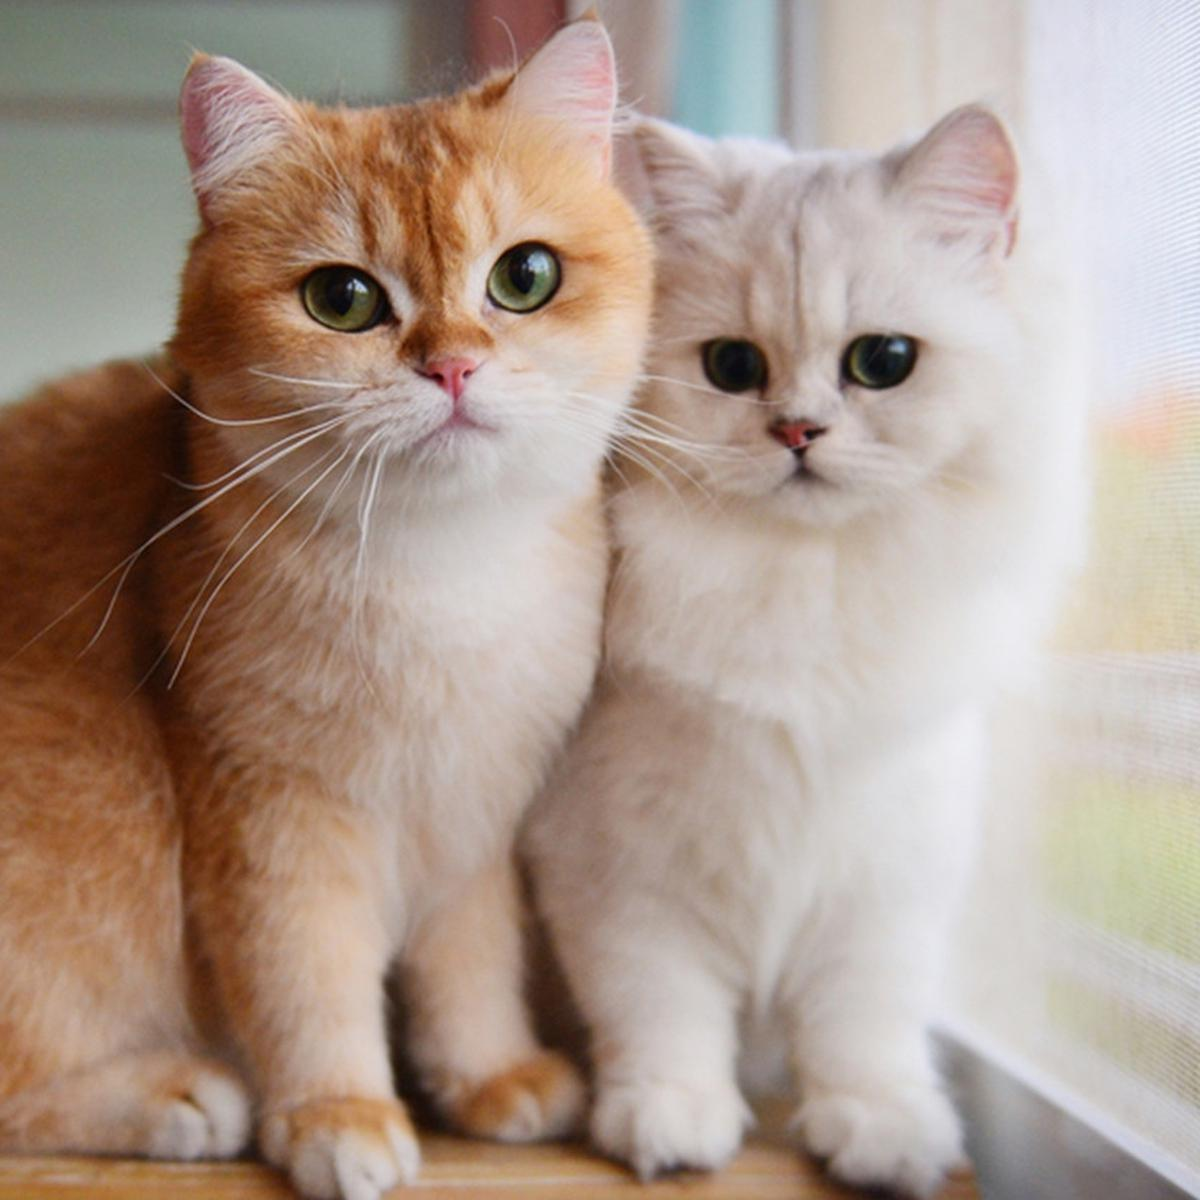
\includegraphics[scale=0.2]{gambar-kucing.jpg}
        \caption{Gambar Kucing Lucu dan Imut}
        \label{fig:kucing}
    \end{figure}
\end{lstlisting}

\noindent Berikut adalah penjelasan dari setiap baris pada kode di atas:

\begin{packed_enum}
    \item \texttt{\textbackslash begin\{figure\}[H] ... \textbackslash end\{figure\}}: Membuat lingkungan \texttt{figure} untuk menyisipkan gambar. Parameter \texttt{[H]} digunakan agar gambar diletakkan tepat di posisi yang ditentukan dalam kode. Opsi \textit{H} dapat diganti dengan \textit{h, t, b, p} sesuai kebutuhan.
    \item \texttt{\textbackslash centering}: Mengatur gambar agar berada di tengah halaman.
    \item \texttt{\textbackslash includegraphics[scale=0.2]\{gambar-kucing.jpg\}}: Memasukkan gambar dengan nama file \texttt{gambar-kucing.jpg}. Parameter \texttt{scale=0.2} mengatur ukuran gambar pada 20\% dari ukuran aslinya. Ubah nilainya untuk memperbesar atau memperkecil gambar.
    \item \texttt{\textbackslash caption\{Gambar Kucing Lucu dan Imut\}}: Menambahkan keterangan (caption) di bawah gambar yang akan muncul di Daftar Gambar dan disertai nomor gambar secara otomatis.
    \item \texttt{\textbackslash label\{fig:kucing\}}: Memberikan label pada gambar untuk merujuk gambar ini dalam teks menggunakan \texttt{\textbackslash cref\{fig:kucing\}} atau \texttt{\textbackslash ref\{fig:kucing\}} yang menghasilkan "Gambar 1" atau penomoran gambar sesuai urutan.
\end{packed_enum}

Hasilnya adalah terlihat seperti pada \cref{fig:kucing}.

\begin{figure}[H]
    \centering
    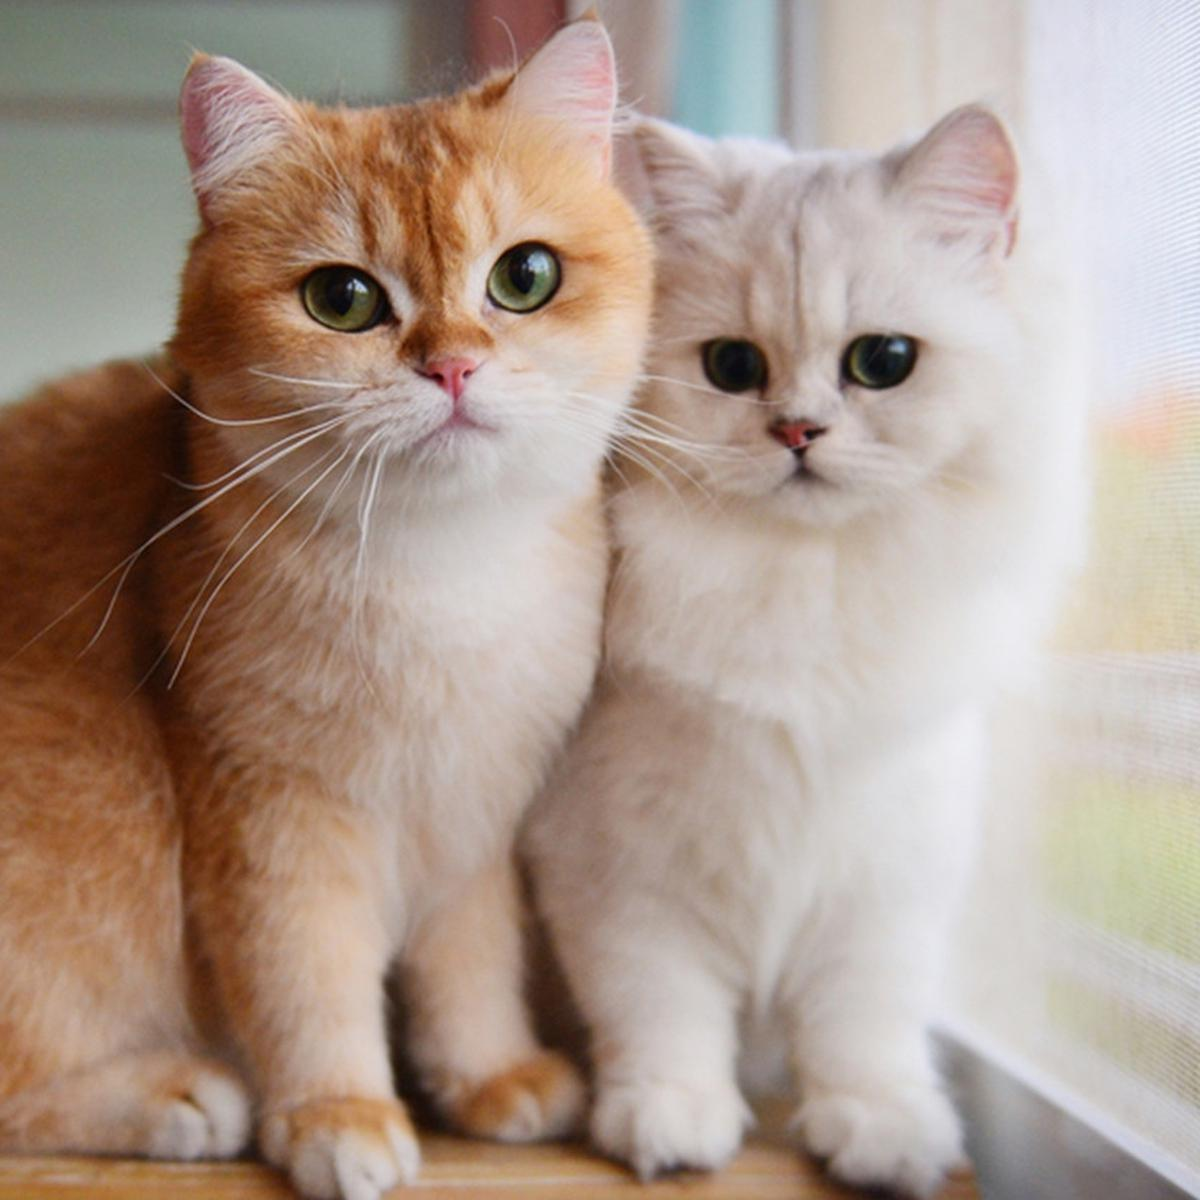
\includegraphics[scale=0.1]{gambar-kucing}
    \caption{Gambar Kucing Lucu dan Imut dengan scala 0.1}
    \label{fig:kucing}
\end{figure}

Setiap gambar harus dimention atau disebutkan didalam bacaan seperti berikut ini \cref{fig:kucing} dan \cref{fig:logoUBS}.

\begin{figure}[H]
    \centering
    
\includegraphics[scale=0.4]{logo-ubs}
    \caption{Logo UBS dengan scala 0.4}
    \label{fig:logoUBS}
\end{figure}

Untuk menyisipkan beberapa gambar dalam satu kelompok dan satu caption utama, kita dapat menggunakan lingkungan \texttt{subfigure} di dalam lingkungan \texttt{figure}. Metode ini sangat bermanfaat jika kita ingin menyusun beberapa gambar berukuran kecil dalam satu baris atau kolom, dengan setiap gambar diberi caption masing-masing dan satu caption utama untuk keseluruhan gambar.

Kode berikut menunjukkan cara menyusun tiga gambar secara berdampingan dengan satu caption utama.

\begin{lstlisting}[language=TeX, caption=Kode untuk Menyisipkan Gambar dalam Dokumen dengan Subfigure, label=lst:kode_gambar_multi]
    \begin{figure}
        \centering
        \begin{subfigure}[b]{0.3\textwidth}
            \centering
            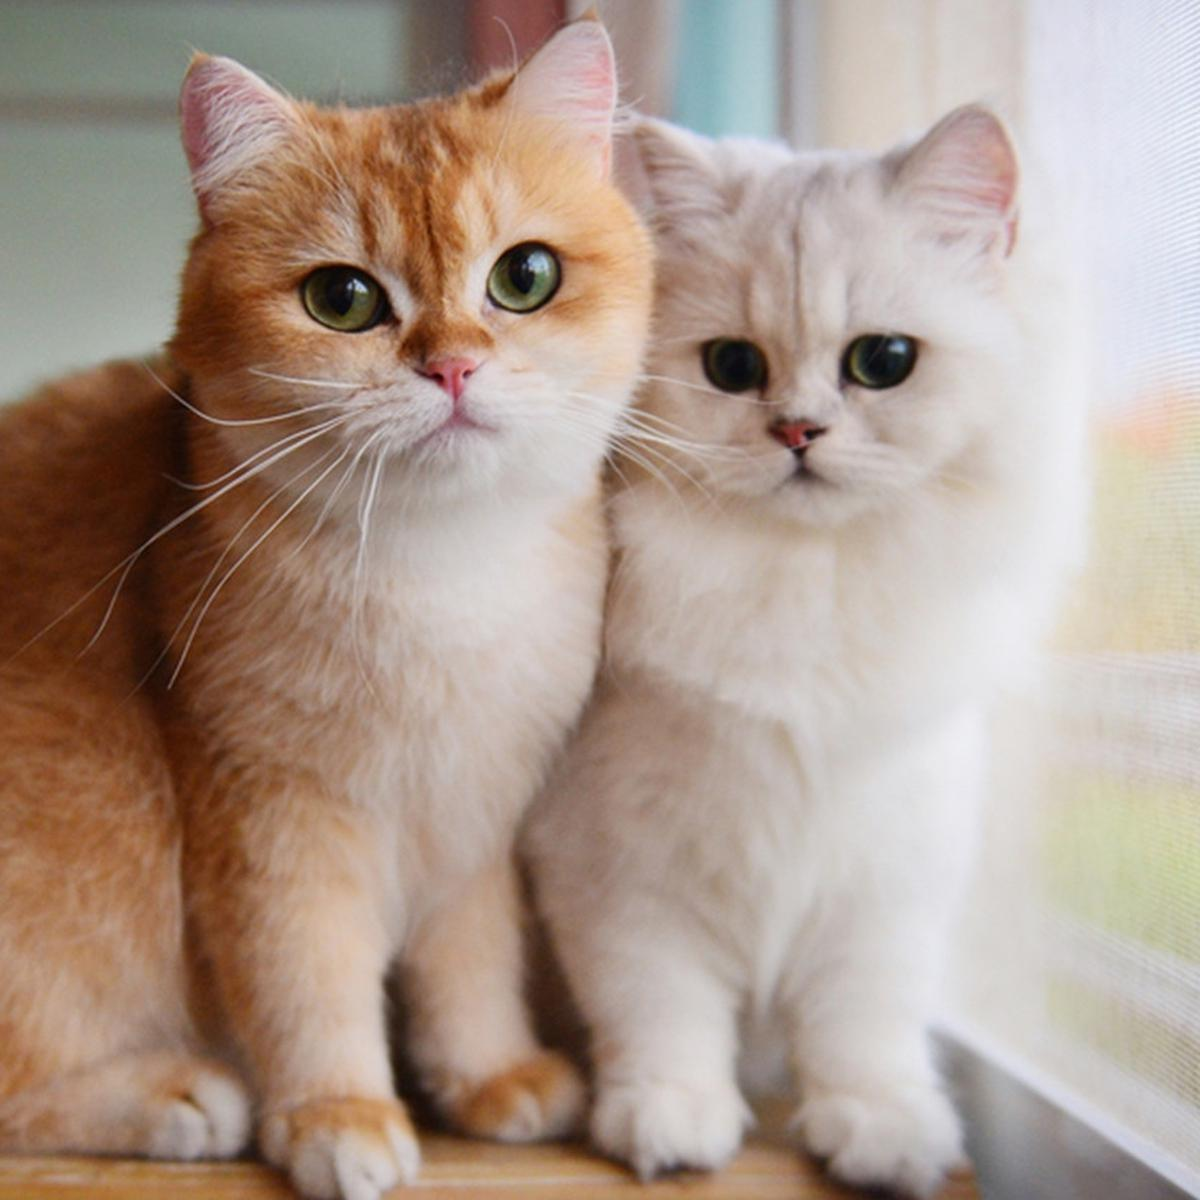
\includegraphics[width=\linewidth]{gambar-kucing.jpg}
            \caption{Kucing Lucu 1}
            \label{fig:kucing-a}
        \end{subfigure}
        \hfill
        \begin{subfigure}[b]{0.3\textwidth}
            \centering
            
\includegraphics[width=\linewidth]{logo-ubs.png}
            \caption{Logo UBS}
            \label{fig:logo-ubs-b}
        \end{subfigure}
        \hfill
        \begin{subfigure}[b]{0.3\textwidth}
            \centering
            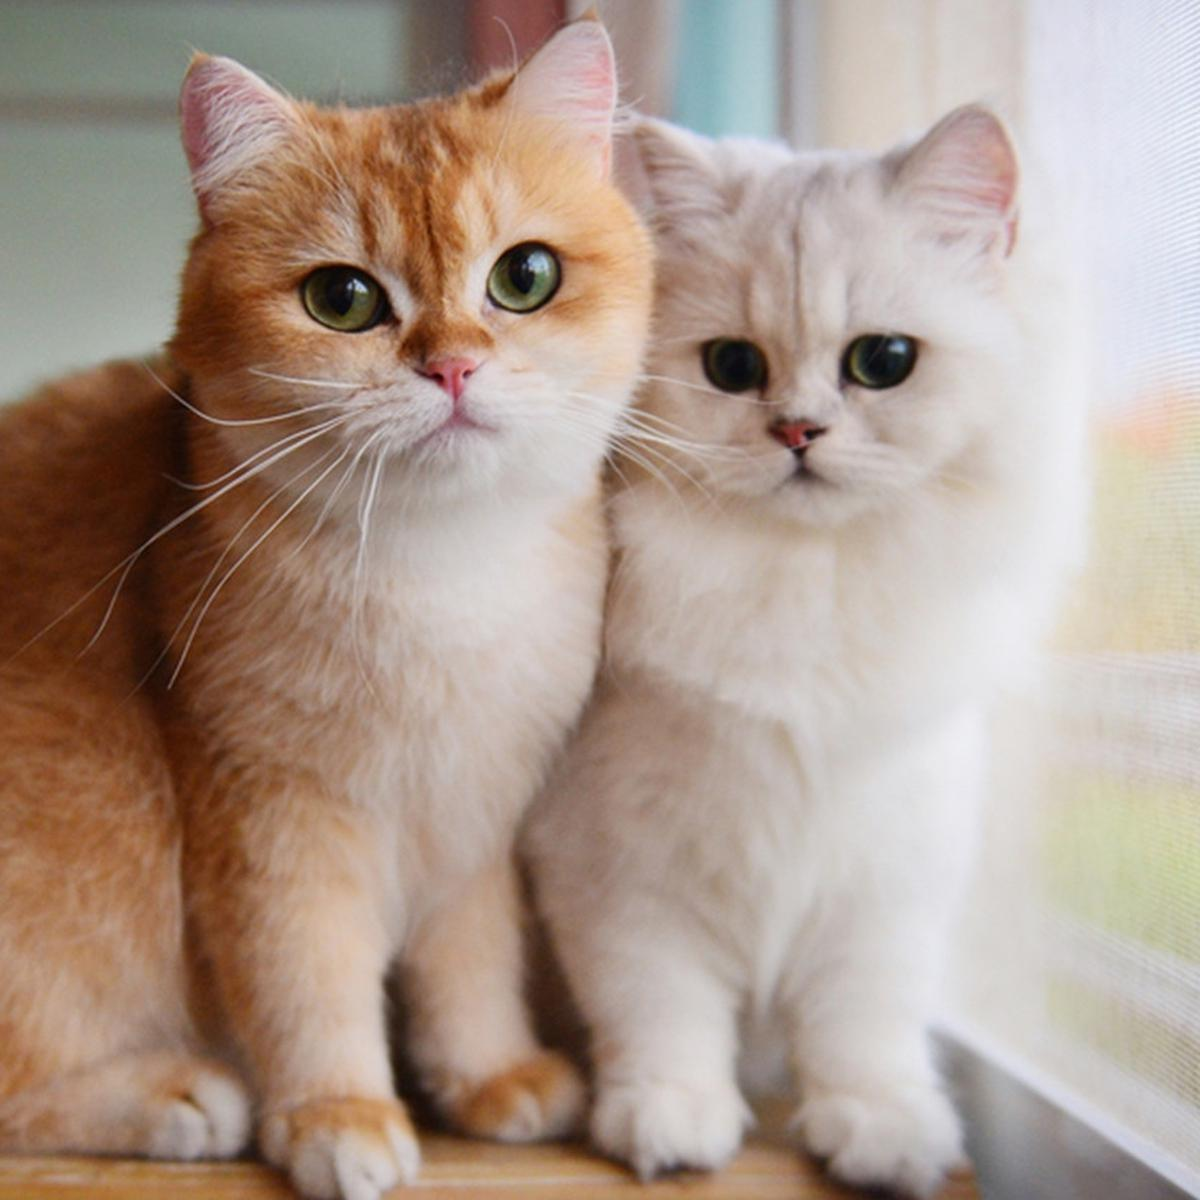
\includegraphics[width=\linewidth]{gambar-kucing.jpg}
            \caption{Kucing Lucu 2}
            \label{fig:kucing-c}
        \end{subfigure}
        \caption{Beberapa gambar yang disusun menjadi 1 bagian dengan penomoran (a), (b), dan (c)}
        \label{fig:kucingdanUBS}
    \end{figure}
\end{lstlisting}

\noindent Berikut adalah penjelasan dari setiap bagian kode di atas:

\begin{packed_enum}
    \item \texttt{\textbackslash begin\{figure\} ... \textbackslash end\{figure\}}: Lingkungan \texttt{figure} utama yang berfungsi sebagai wadah untuk menyisipkan beberapa gambar dalam satu bagian.
    
    \item \texttt{\textbackslash begin\{subfigure\}[b]\{0.3\textbackslash textwidth\} ... \textbackslash end\{subfigure\}}: Lingkungan \texttt{subfigure} digunakan untuk setiap gambar yang ingin disusun dalam satu bagian. Parameter \texttt{0.3\textbackslash textwidth} mengatur lebar setiap gambar menjadi sepertiga dari lebar teks, sehingga tiga gambar dapat ditampilkan berdampingan dalam satu baris.
    
    \item \texttt{\textbackslash includegraphics[width=\textbackslash linewidth]\{gambar-nama\}}: Memasukkan setiap gambar dengan lebar yang sesuai dengan lebar yang telah ditentukan untuk \texttt{subfigure}. 
        \begin{packed_enum}
            \item Gambar pertama menggunakan file \texttt{gambar-kucing}, dengan caption "Kucing Lucu 1".
            \item Gambar kedua menggunakan file \texttt{logo-ubs}, dengan caption "Logo UBS".
            \item Gambar ketiga juga menggunakan file \texttt{gambar-kucing}, dengan caption "Kucing Lucu 2".
        \end{packed_enum}
    
    \item \texttt{\textbackslash hfill}: Menyisipkan ruang kosong antar gambar, agar setiap \texttt{subfigure} memiliki jarak yang merata.
    
    \item \texttt{\textbackslash caption\{...\}}: Caption utama yang menjelaskan ketiga gambar sekaligus. Caption ini akan ditampilkan di bawah semua gambar dalam lingkungan \texttt{figure}.

    \item \texttt{\textbackslash label\{fig:kucingdanUBS\}}: Memberikan label untuk keseluruhan kelompok gambar, sehingga kita bisa merujuk ke seluruh bagian gambar ini dalam teks dengan \texttt{\textbackslash cref\{fig:kucingdanUBS\}}.
\end{packed_enum}

Dengan menggunakan metode ini, Anda dapat menyisipkan beberapa gambar dalam satu bagian dengan satu caption utama seperti pada \cref{fig:kucingdanUBS}. Setiap gambar dapat memiliki caption terpisah dan nomor (misalnya, (a), (b), (c)), sehingga rujukan spesifik untuk masing-masing gambar dapat dibuat, seperti \texttt{\textbackslash cref\{fig:kucing-a\}} untuk merujuk ke \cref{fig:kucing-a}.

\begin{figure}
    \centering
    \begin{subfigure}[b]{0.3\textwidth}
        \centering
        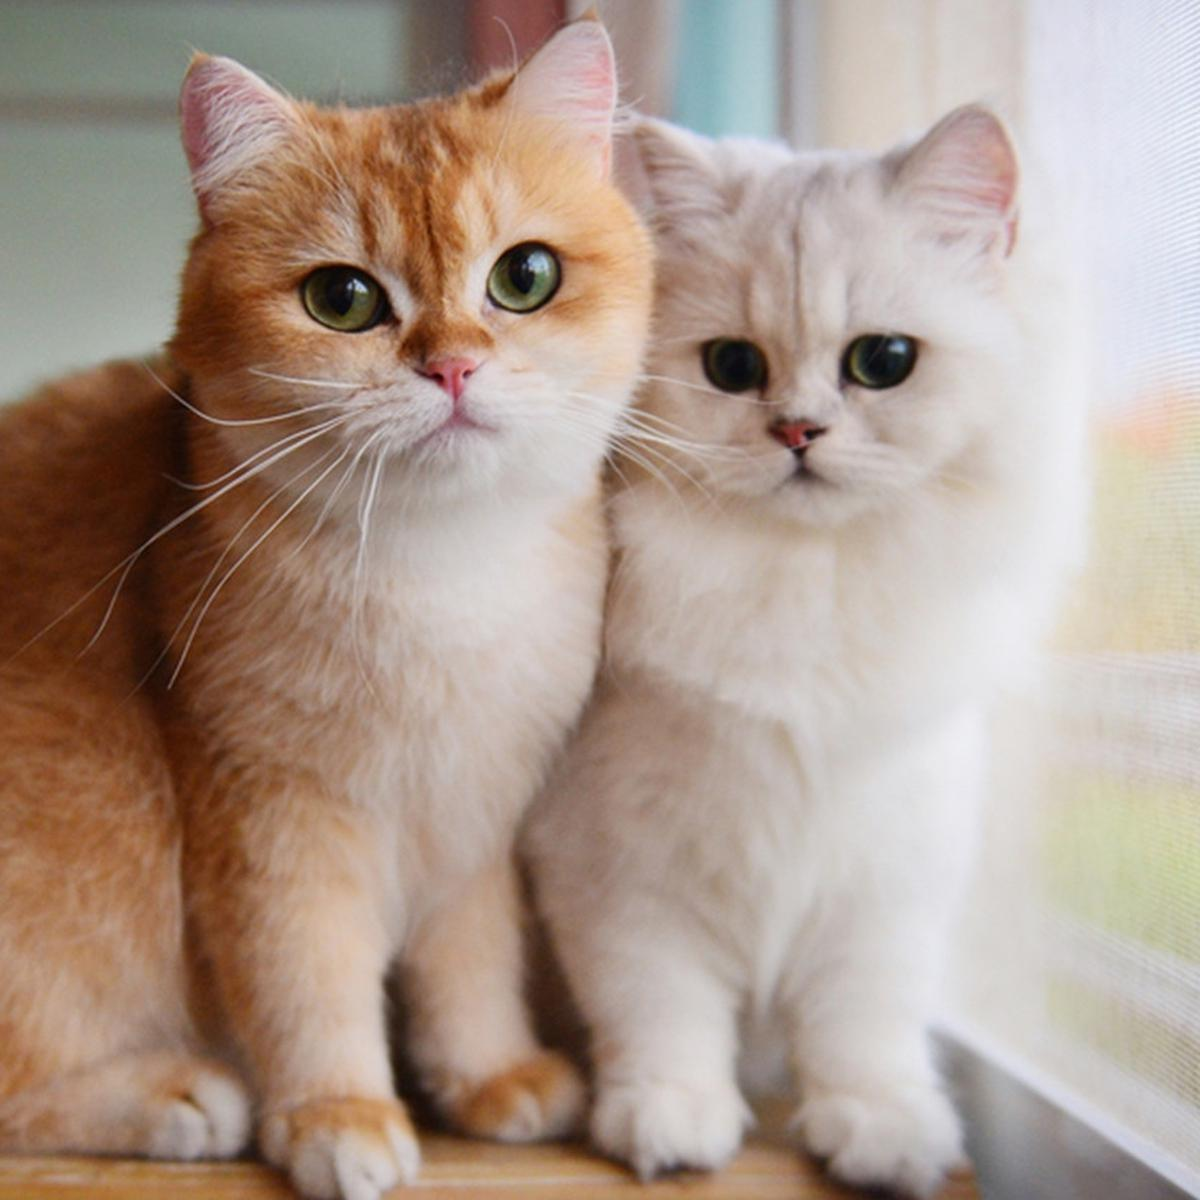
\includegraphics[width=\linewidth]{gambar-kucing.jpg}
        \caption{Kucing Lucu 1}
        \label{fig:kucing-a}
    \end{subfigure}
    \hfill
    \begin{subfigure}[b]{0.3\textwidth}
        \centering
        
\includegraphics[width=\linewidth]{logo-ubs.png}
        \caption{Logo UBS}
        \label{fig:logo-ubs-b}
    \end{subfigure}
    \hfill
    \begin{subfigure}[b]{0.3\textwidth}
        \centering
        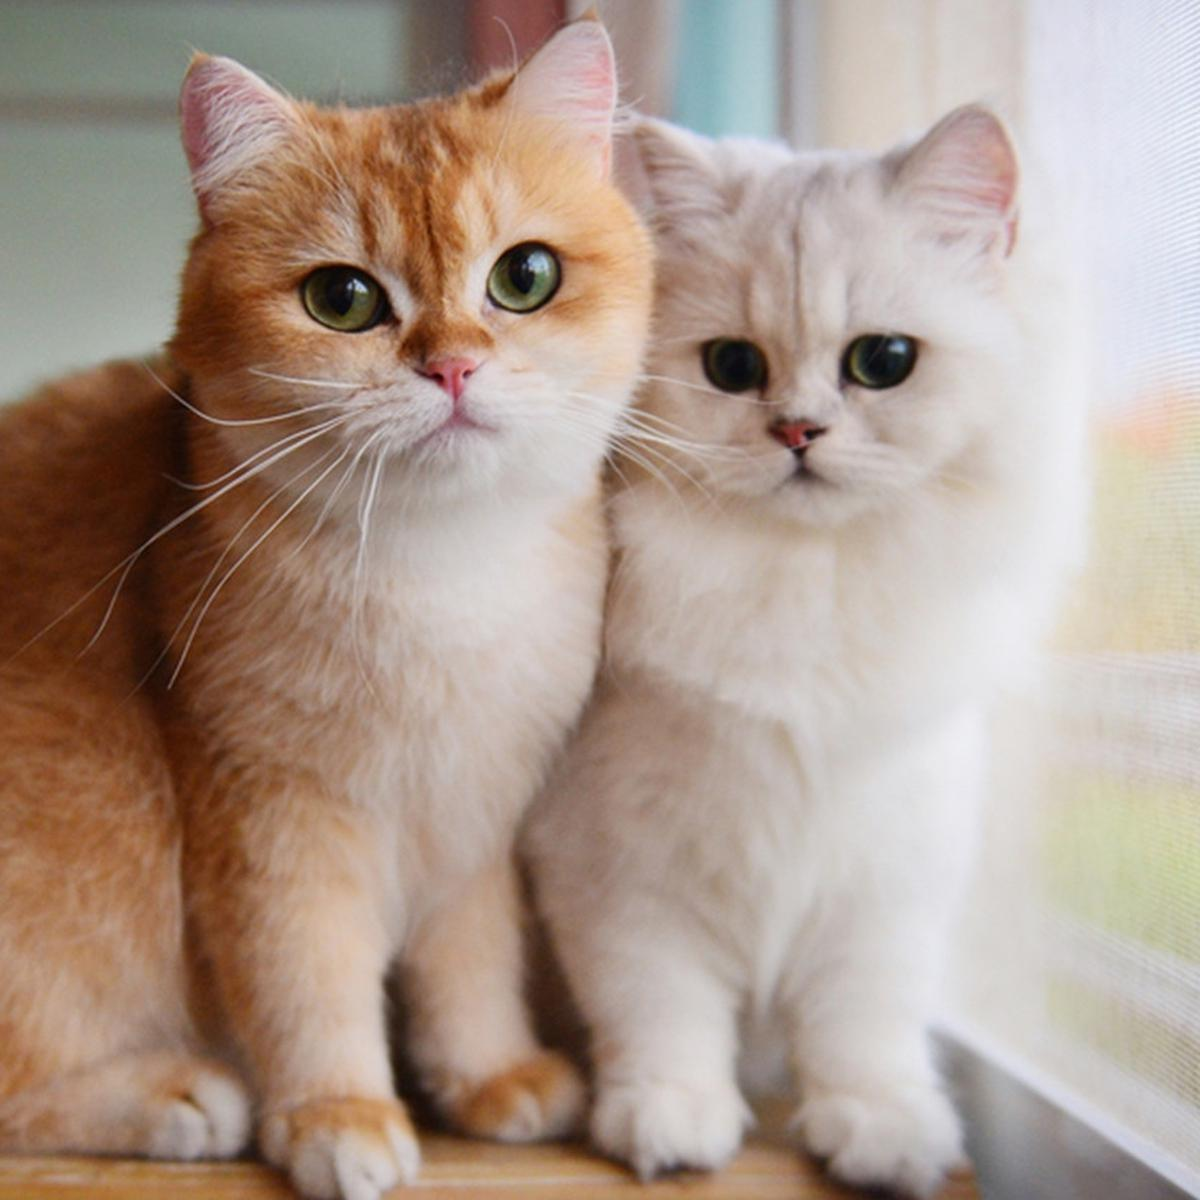
\includegraphics[width=\linewidth]{gambar-kucing.jpg}
        \caption{Kucing Lucu 2}
        \label{fig:kucing-c}
    \end{subfigure}
    \caption{Beberapa gambar yang disusun menjadi 1 bagian dengan penomoran (a), (b), dan (c)}
    \label{fig:kucingdanUBS}
\end{figure}

\section{Membuat Grafik dengan Tikz}
TikZ adalah sebuah paket LaTeX yang digunakan untuk membuat grafik vektor. Berikut adalah beberapa contoh dasar penggunaan TikZ.

\subsection{Menggambar Garis dan Bentuk Dasar}
Untuk menggambar garis dan bentuk dasar, kita bisa menggunakan perintah-perintah berikut:
\begin{lstlisting}[language=TeX, caption=Kode untuk Menggambar Garis dan Bentuk Dasar, label=lst:Menggambar Garis dan Bentuk Dasar]
    \begin{figure}[H]
        \centering
        \begin{tikzpicture}
            \draw (0,0) -- (2,0);
            \draw (0,0) rectangle (2,2);
            \draw (1,1) circle (1);
        \end{tikzpicture}
        \caption{Menggambar Garis dan Bentuk Dasar}
        \label{fig:tikzExample}
    \end{figure}
\end{lstlisting}

\begin{figure}[H]
    \centering
    \begin{tikzpicture}
        \draw (0,0) -- (2,0);
        \draw (0,0) rectangle (2,2);
        \draw (1,1) circle (1);
    \end{tikzpicture}
    \caption{Menggambar Garis dan Bentuk Dasar}
    \label{fig:tikzExample}
\end{figure}

Pada Gambar \ref{fig:tikzExample} dapat dilihat contoh gambar sederhana.

\subsection{Menggambar Grafik Fungsi}
TikZ juga bisa digunakan untuk menggambar grafik fungsi matematika:
\begin{lstlisting}[language=TeX, caption=Kode untuk Menggambar Grafik Fungsi, label=lst:Menggambar Grafik Fungsi]
    \begin{figure}[H]
        \centering
        \begin{tikzpicture}
            \begin{axis}[
                axis lines = middle,
                xlabel = $x$,
                ylabel = {$f(x)$},
                title = {Grafik Fungsi Kuadrat},
                grid = major,
                xmin = -10, 
                xmax = 10,
                ymin = 0, 
                ymax = 100
            ]
            \addplot [
                domain=-10:10, 
                samples=100, 
                color=blue,
            ]
            {x^2};
            \end{axis}
        \end{tikzpicture}
        \caption{Grafik fungsi \( f(x) = x^2 \) dengan domain \( [-10, 10] \)}
        \label{fig:grafik_kuadrat}
    \end{figure}
\end{lstlisting}

\begin{figure}[H]
    \centering
    \begin{tikzpicture}
        \begin{axis}[
            axis lines = middle,
            xlabel = $x$,
            ylabel = {$f(x)$},
            title = {Grafik Fungsi Kuadrat},
            grid = major,
            xmin = -10, 
            xmax = 10,
            ymin = 0, 
            ymax = 100
        ]
        \addplot [
            domain=-10:10, 
            samples=100, 
            color=blue,
        ]
        {x^2};
        \end{axis}
    \end{tikzpicture}
    \caption{Grafik fungsi \( f(x) = x^2 \) dengan domain \( [-10, 10] \)}
    \label{fig:grafik_kuadrat}
\end{figure}

Pada Gambar \ref{fig:grafik_kuadrat} ditunjukkan grafik fungsi kuadrat.

\subsection{Menggambar Diagram Alir}
TikZ juga mendukung pembuatan diagram alir (flowchart):
\begin{lstlisting}[language=TeX, caption=Kode untuk Menggambar Diagram Alir, label=lst:Menggambar Diagram Alir]
    \begin{figure}[H]
        \centering
        \begin{tikzpicture}[node distance=2cm]
            \node (start) [startstop] {Start};
            \node (process1) [process, below of=start] {Process 1};
            \node (decision) [decision, below of=process1] {Decision};
            \node (process2a) [process, below of=decision, yshift=-1cm] {Process 2a};
            \node (process2b) [process, right of=decision, xshift=2cm] {Process 2b};
            \node (stop) [startstop, below of=process2a] {Stop};
    
            \draw [arrow] (start) -- (process1);
            \draw [arrow] (process1) -- (decision);
            \draw [arrow] (decision) -- node[anchor=east] {yes} (process2a);
            \draw [arrow] (decision) -- node[anchor=south] {no} (process2b);
            \draw [arrow] (process2a) -- (stop);
        \end{tikzpicture}
        \caption{Diagram alir sederhana dengan kondisi percabangan}
        \label{fig:flowchart_sederhana}
    \end{figure}
\end{lstlisting}
\begin{figure}[H]
    \centering
    \begin{tikzpicture}[node distance=2cm]
        \node (start) [startstop] {Start};
        \node (process1) [process, below of=start] {Process 1};
        \node (decision) [decision, below of=process1] {Decision};
        \node (process2a) [process, below of=decision, yshift=-1cm] {Process 2a};
        \node (process2b) [process, right of=decision, xshift=2cm] {Process 2b};
        \node (stop) [startstop, below of=process2a] {Stop};

        \draw [arrow] (start) -- (process1);
        \draw [arrow] (process1) -- (decision);
        \draw [arrow] (decision) -- node[anchor=east] {yes} (process2a);
        \draw [arrow] (decision) -- node[anchor=south] {no} (process2b);
        \draw [arrow] (process2a) -- (stop);
    \end{tikzpicture}
    \caption{Diagram alir sederhana dengan kondisi percabangan}
    \label{fig:flowchart_sederhana}
\end{figure}
Pada Gambar \ref{fig:flowchart_sederhana} ditunjukkan contoh diagram alir sederhana dengan satu kondisi percabangan.

\subsection{Menggambar Grafik Batang}
Untuk menggambar grafik batang, kita bisa menggunakan perintah berikut:
\begin{lstlisting}[language=TeX, caption=Kode untuk Menggambar Grafik Batang, label=lst:Menggambar Grafik Batang]
    \begin{figure}[H]
        \centering
        \begin{tikzpicture}
            \begin{axis}[
                ybar,
                symbolic x coords={A, B, C, D},
                xtick=data,
                ylabel={Nilai},
                xlabel={Kategori},
                title={Grafik Batang Sederhana},
                bar width=0.5cm,
                ymin=0,
                ymajorgrids=true
            ]
            \addplot[fill=blue!50] coordinates {(A,1) (B,3) (C,2) (D,4)};
            \end{axis}
        \end{tikzpicture}
        \caption{Grafik batang yang menunjukkan nilai untuk kategori A, B, C, dan D}
        \label{fig:grafik_batang}
    \end{figure}
\end{lstlisting}
\begin{figure}[H]
    \centering
    \begin{tikzpicture}
        \begin{axis}[
            ybar,
            symbolic x coords={A, B, C, D},
            xtick=data,
            ylabel={Nilai},
            xlabel={Kategori},
            title={Grafik Batang Sederhana},
            bar width=0.5cm,
            ymin=0,
            ymajorgrids=true
        ]
        \addplot[fill=blue!50] coordinates {(A,1) (B,3) (C,2) (D,4)};
        \end{axis}
    \end{tikzpicture}
    \caption{Grafik batang yang menunjukkan nilai untuk kategori A, B, C, dan D}
    \label{fig:grafik_batang}
\end{figure}
Pada Gambar \ref{fig:grafik_batang} dapat dilihat distribusi nilai pada berbagai kategori.

\subsection{Menggambar Grafik Pie}
TikZ juga mendukung pembuatan grafik pie:
\begin{lstlisting}[language=TeX, caption=Kode untuk Menggambar Grafik Pie, label=lst:Menggambar Grafik Pie]
    \begin{figure}[H]
        \centering
        \begin{tikzpicture}
            \pie{30/A, 20/B, 50/C}
        \end{tikzpicture}
        \caption{Diagram lingkaran yang menunjukkan distribusi persentase A, B, dan C}
        \label{fig:pie_chart}
    \end{figure}
\end{lstlisting}
\begin{figure}[H]
    \centering
    \begin{tikzpicture}
        \pie{30/A, 20/B, 50/C}
    \end{tikzpicture}
    \caption{Diagram lingkaran yang menunjukkan distribusi persentase A, B, dan C}
    \label{fig:pie_chart}
\end{figure}
Pada Gambar \ref{fig:pie_chart} ditunjukkan pembagian persentase untuk kategori A, B, dan C.

Dengan contoh-contoh di atas, Anda dapat mulai membuat berbagai jenis grafik menggunakan TikZ di \LaTeX. Untuk informasi lebih lanjut, Anda dapat merujuk ke dokumentasi resmi TikZ.

\section{Membuat Tabel}
Pada bagian ini akan dijelaskan bagaimana membuat tabel dalam sebuah dokumen \LaTeX. untuk membuat tabel memang agak sedikit sulit, sehingga saya menyarankan menggunakan tool berikut \url{https://www.tablesgenerator.com/} atau \url{https://www.latex-tables.com/} kemudian isikan tabel pada tool generator tersebut dan salin kodenya ke dalam dokumen \LaTeX. Berikut adalah contoh dari sebuah tabel yang telah dibuat. Jangan lupa setiap tabel harus dimention dan dijelaskan dibacaan seperti berikut ini \cref{tab:hresult}. Contoh pembuatan tabel terlihat kodenya pada \cref{lst:kode_tabel}.

\begin{lstlisting}[language=TeX, caption=Kode untuk Membuat Tabel dalam Dokumen, label=lst:kode_tabel]
    \begin{table}[h]
        \caption{Performance Using Hard Decision Detection}
        \label{tab:hresult}
        \centering
        \begin{tabular}{c rrrrrrr}
            \hline\hline
            Audio Name&\multicolumn{7}{c}{Sum of Extracted Bits} \\ [0.5ex] 
            \hline
            Police & 5 & -1 & 5& 5& -7& -5& 3\\
            Midnight & 7 & -3 & 5& 3& -1& -3& 5\\
            News & 9 & -3 & 7& 9& -5& -1& 9\\[0.8ex]
            \hline
        \end{tabular}
    \end{table}
\end{lstlisting}

\noindent Berikut adalah penjelasan dari setiap bagian kode di atas:

\begin{packed_enum}
    \item \texttt{\textbackslash begin\{table\}[h] ... \textbackslash end\{table\}}: Lingkungan \texttt{table} digunakan untuk membuat tabel dan menempatkannya di posisi tertentu dalam dokumen. Parameter \texttt{[h]} menginstruksikan LaTeX untuk menempatkan tabel di posisi yang paling mendekati lokasi kode tersebut dalam teks. Jika posisi ini tidak berfungsi dengan baik, Anda bisa menggunakan parameter lain, seperti \texttt{[H]} (dari paket \texttt{float}) untuk menempatkan tabel di lokasi yang lebih spesifik.
    \item \texttt{\textbackslash caption\{Performance Using Hard Decision Detection\}}: Menambahkan keterangan (caption) di atas tabel. Caption ini akan otomatis ditampilkan dalam Daftar Tabel dan diberi nomor secara otomatis oleh LaTeX.
    \item \texttt{\textbackslash label\{tab:hresult\}}: Memberi label pada tabel, memungkinkan tabel dirujuk dalam teks menggunakan perintah \texttt{\textbackslash cref\{tab:hresult\}} atau \texttt{\textbackslash ref\{tab:hresult\}}, yang akan menghasilkan "Tabel 1" atau sesuai penomoran tabel.
    \item \texttt{\textbackslash centering}: Mengatur tabel agar berada di tengah halaman.
    \item \texttt{\textbackslash begin\{tabular\}\{c rrrrrrr\} ... \textbackslash end\{tabular\}}: Lingkungan \texttt{tabular} digunakan untuk membuat struktur tabel. Pengaturan kolom menggunakan karakter:
        \begin{packed_enum}
            \item \texttt{c}: Mengatur kolom pertama rata tengah.
            \item \texttt{r}: Mengatur tujuh kolom berikutnya rata kanan.
        \end{packed_enum}
    \item \texttt{\textbackslash hline}: Menambahkan garis horizontal di tabel. Dua \texttt{\textbackslash hline} berturut-turut digunakan untuk garis ganda pada bagian header tabel.
    \item \texttt{\textbackslash multicolumn\{7\}\{c\}\{Sum of Extracted Bits\}}: Menggabungkan tujuh kolom berikutnya menjadi satu sel besar yang berisi teks "Sum of Extracted Bits", yang disejajarkan ke tengah dengan pengaturan \texttt{c}.
    \item Isi tabel, seperti:
        \begin{packed_enum}
            \item \texttt{Police}: Data pada baris ini terkait audio "Police", dengan tujuh angka di kolom berikutnya yang merepresentasikan "Sum of Extracted Bits".
            \item Baris lain mengikuti format yang sama.
        \end{packed_enum}
    \item Jarak tambahan antara baris terakhir dan \texttt{\textbackslash hline} berikutnya diberikan dengan parameter opsional \texttt{[0.8ex]}, yang menambahkan spasi vertikal untuk keterbacaan.
\end{packed_enum}

Dengan penjelasan ini, kode menghasilkan tabel terstruktur yang diberi nomor secara otomatis dan dapat dirujuk di teks dokumen. Hasil tabel dari \cref{lst:kode_tabel} adalah terlihat pada \cref{tab:hresult}.

\begin{table}[h]
    \caption{Performance Using Hard Decision Detection}
    \label{tab:hresult}
    \centering
    \begin{tabular}{c rrrrrrr}
        \hline\hline
        Audio Name&\multicolumn{7}{c}{Sum of Extracted Bits} \\ [0.5ex] 
        \hline
        Police & 5 & -1 & 5& 5& -7& -5& 3\\
        Midnight & 7 & -3 & 5& 3& -1& -3& 5\\
        News & 9 & -3 & 7& 9& -5& -1& 9\\[0.8ex]
        \hline
    \end{tabular}
\end{table}

Kita juga bisa menambahkan tabel yang besar dengan format halaman landscape seperti contoh berikut dan mention tabel seperti berikut ini \cref{tab:LPer} dan berikut ini \cref{tab:PPer}.

\begin{lstlisting}[language=TeX, caption=Kode untuk Membuat Tabel dalam Dokumen dengan Sideway, label=lst:kode_tabel_sideway]
    \begin{sidewaystable}[htbp]
        \caption{Performance After Post Filtering}
        \label{tab:LPer}
        \centering
        \begin{tabular}{l c c rrrrrrr}
            \hline\hline
            Audio &Audibility & Decision &\multicolumn{7}{c}{Sum of Extracted Bits} 
            \\ [0.5ex] 
            \hline
            & &soft &1 & $-1$ & 1 & 1 & $-1$ & $-1$ & 1 \\[-1ex]
            \raisebox{1.5ex}{Police} & \raisebox{1.5ex}{5}&hard
            & 2 & $-4$ & 4 & 4 & $-2$ & $-4$ & 4 \\[1ex]
            & &soft & 1 & $-1$ & 1 & 1 & $-1$ & $-1$ & 1 \\[-1ex]
            \raisebox{1.5ex}{Beethoven} & \raisebox{1.5ex}{5}& hard
            &8 & $-8$ & 2 & 8 & $-8$ & $-8$ & 6 \\[1ex]
            & &soft & 1 & $-1$ & 1 & 1 & $-1$ & $-1$ & 1 \\[-1ex]
            \raisebox{1.5ex}{Metallica} & \raisebox{1.5ex}{5}& hard
            &4 & $-8$ & 8 & 4 & $-8$ & $-8$ & 8 \\[1ex]
            \hline
        \end{tabular}
    \end{sidewaystable}
\end{lstlisting}

\noindent Berikut adalah penjelasan dari setiap bagian kode di atas:

\begin{packed_enum}
    \item \texttt{\textbackslash begin\{sidewaystable\}[htbp] ... \textbackslash end\{sidewaystable\}}: Lingkungan \texttt{sidewaystable} dari paket \texttt{rotating} digunakan untuk menampilkan tabel dalam orientasi landscape. Parameter \texttt{[htbp]} menunjukkan preferensi posisi tabel pada dokumen. Pastikan Anda telah memuat paket \texttt{rotating} di preamble dengan perintah \texttt{\textbackslash usepackage\{rotating\}}.
    \item \texttt{\textbackslash caption\{Performance After Post Filtering\}}: Menambahkan caption (keterangan) di atas tabel. Caption ini akan otomatis dimasukkan dalam Daftar Tabel dan diberi nomor secara otomatis.
    \item \texttt{\textbackslash label\{tab:LPer\}}: Memberi label pada tabel, memungkinkan Anda merujuk tabel ini dalam teks menggunakan perintah \texttt{\textbackslash cref\{tab:LPer\}} atau \texttt{\textbackslash ref\{tab:LPer\}}, yang akan menghasilkan "Tabel 1" atau sesuai penomoran tabel.
    \item \texttt{\textbackslash centering}: Mengatur tabel agar berada di tengah halaman.
    \item \texttt{\textbackslash begin\{tabular\}\{l c c rrrrrrr\} ... \textbackslash end\{tabular\}}: Lingkungan \texttt{tabular} digunakan untuk membuat struktur tabel dengan pengaturan kolom sebagai berikut:
        \begin{packed_enum}
            \item \texttt{l}: Mengatur kolom pertama rata kiri untuk kolom "Audio".
            \item \texttt{c}: Mengatur kolom kedua dan ketiga rata tengah untuk kolom "Audibility" dan "Decision".
            \item \texttt{r}: Tujuh kolom berikutnya rata kanan untuk data "Sum of Extracted Bits".
        \end{packed_enum}
    \item \texttt{\textbackslash hline}: Menambahkan garis horizontal di tabel. Dua \texttt{\textbackslash hline} berturut-turut digunakan untuk garis ganda pada bagian header tabel.
    \item \texttt{\textbackslash multicolumn\{7\}\{c\}\{Sum of Extracted Bits\}}: Menggabungkan tujuh kolom berikutnya menjadi satu sel besar yang berisi teks "Sum of Extracted Bits", yang disejajarkan ke tengah dengan pengaturan \texttt{c}.
    \item Isi tabel, misalnya:
        \begin{packed_enum}
            \item Data pada baris pertama terkait audio "Police", dengan kolom audibility berisi nilai 5, dan data decision dengan dua opsi: "soft" dan "hard".
            \item Data "soft" pada baris pertama dan "hard" pada baris kedua diisi dengan angka sesuai kolom masing-masing.
            \item Untuk beberapa entri seperti "Police", "Beethoven", dan "Metallica", kolom audibility dan audio di tengah (seperti nilai 5) diangkat dengan perintah \texttt{\textbackslash raisebox} untuk memberikan efek centering pada teks.
        \end{packed_enum}
    \item \texttt{[1ex]} atau \texttt{[-1ex]}: Mengatur jarak antar baris untuk menjaga keterbacaan dan posisi elemen tabel yang lebih seimbang.
\end{packed_enum}

Kode ini akan menghasilkan tabel landscape dengan satu caption, beberapa kolom gabungan, dan penomoran otomatis dan hasilnya terlihat pada \cref{tab:LPer}.

\begin{sidewaystable}[htbp]
    \caption{Performance After Post Filtering}
    \label{tab:LPer}
    \centering
    \begin{tabular}{l c c rrrrrrr}
        \hline\hline
        Audio &Audibility & Decision &\multicolumn{7}{c}{Sum of Extracted Bits} 
        \\ [0.5ex] 
        \hline
        & &soft &1 & $-1$ & 1 & 1 & $-1$ & $-1$ & 1 \\[-1ex]
        \raisebox{1.5ex}{Police} & \raisebox{1.5ex}{5}&hard
        & 2 & $-4$ & 4 & 4 & $-2$ & $-4$ & 4 \\[1ex]
        & &soft & 1 & $-1$ & 1 & 1 & $-1$ & $-1$ & 1 \\[-1ex]
        \raisebox{1.5ex}{Beethoven} & \raisebox{1.5ex}{5}& hard
        &8 & $-8$ & 2 & 8 & $-8$ & $-8$ & 6 \\[1ex]
        & &soft & 1 & $-1$ & 1 & 1 & $-1$ & $-1$ & 1 \\[-1ex]
        \raisebox{1.5ex}{Metallica} & \raisebox{1.5ex}{5}& hard
        &4 & $-8$ & 8 & 4 & $-8$ & $-8$ & 8 \\[1ex]
        \hline
    \end{tabular}
\end{sidewaystable}

Contoh lain \cref{lst:kode_tabel_lain} untuk pembuatan tabel seperti di bawah ini dan hasilnya tertampil pada \cref{tab:PPer}.

\begin{lstlisting}[language=TeX, caption=Kode untuk Membuat Tabel dalam Dokumen, label=lst:kode_tabel_lain]
    \begin{table}[ht]
        \caption{Performance After Post Filtering}
        \label{tab:PPer}
        \centering
        \begin{tabular}{l c c rrrrrrr}
            \hline\hline
            Audio &Audibility & Decision &\multicolumn{7}{c}{Sum of Extracted Bits} 
            \\ [0.5ex] 
            \hline
            & &soft &1 & $-1$ & 1 & 1 & $-1$ & $-1$ & 1 \\[-1ex]
            \raisebox{1.5ex}{Police} & \raisebox{1.5ex}{5}&hard
            & 2 & $-4$ & 4 & 4 & $-2$ & $-4$ & 4 \\[1ex]
            & &soft & 1 & $-1$ & 1 & 1 & $-1$ & $-1$ & 1 \\[-1ex]
            \raisebox{1.5ex}{Beethoven} & \raisebox{1.5ex}{5}& hard
            &8 & $-8$ & 2 & 8 & $-8$ & $-8$ & 6 \\[1ex]
            & &soft & 1 & $-1$ & 1 & 1 & $-1$ & $-1$ & 1 \\[-1ex]
            \raisebox{1.5ex}{Metallica} & \raisebox{1.5ex}{5}& hard
            &4 & $-8$ & 8 & 4 & $-8$ & $-8$ & 8 \\[1ex]
            \hline
        \end{tabular}
    \end{table}
\end{lstlisting}

\begin{table}[ht]
	\caption{Performance After Post Filtering}
	\label{tab:PPer}
	\centering
	\begin{tabular}{l c c rrrrrrr}
		\hline\hline
		Audio &Audibility & Decision &\multicolumn{7}{c}{Sum of Extracted Bits} 
		\\ [0.5ex] 
		\hline
		& &soft &1 & $-1$ & 1 & 1 & $-1$ & $-1$ & 1 \\[-1ex]
		\raisebox{1.5ex}{Police} & \raisebox{1.5ex}{5}&hard
		& 2 & $-4$ & 4 & 4 & $-2$ & $-4$ & 4 \\[1ex]
		& &soft & 1 & $-1$ & 1 & 1 & $-1$ & $-1$ & 1 \\[-1ex]
		\raisebox{1.5ex}{Beethoven} & \raisebox{1.5ex}{5}& hard
		&8 & $-8$ & 2 & 8 & $-8$ & $-8$ & 6 \\[1ex]
		& &soft & 1 & $-1$ & 1 & 1 & $-1$ & $-1$ & 1 \\[-1ex]
		\raisebox{1.5ex}{Metallica} & \raisebox{1.5ex}{5}& hard
		&4 & $-8$ & 8 & 4 & $-8$ & $-8$ & 8 \\[1ex]
		\hline
	\end{tabular}
\end{table}

\section{Menambahkan Persamaan}

Persamaan tidak lepas dari bidang ilmu teknik dan kadang perlu dituliskan dalam sebuah laporan. Sangat mudah menuliskan persamaan pada sebuah dokumen \LaTeX. Terdapat 2 jenis penulisan persamaan, yaitu inline dengan text seperti contoh ini \(x^2 + y^2 = z^2\) atau seperti ini $E=mc^2$. Jenis lain adalah dituliskan seperti di bawah ini, yang otomatis akan mendapatkan penomoran. Apabila belum familiar dengan kode untuk penulisan persamaan pada \LaTeX, Anda bisa menggunakan tool berikut \url{https://latex.codecogs.com/eqneditor/editor.php} atau \url{https://latexeditor.lagrida.com/}. Setiap persamaan harus disebutkan dalam teks seperti \cref{eq:satu} dan \cref{eq:equationDua} dan dijelaskan terkait persamaan tersebut untuk apa.

\begin{lstlisting}[language=TeX, caption=Kode untuk Menulis Persamaan, label=lst:kode_persamaan_emc]
    \begin{equation}
        \label{eq:satu}
        E=mc^2
    \end{equation}
\end{lstlisting}

\begin{lstlisting}[language=TeX, caption=Kode untuk Menulis Persamaan, label=lst:kode_persamaan_mn]
    \begin{equation}
        \label{eq:equationDua}
        m_n = k_p*e_n + \frac{k_e*T}{T_{reset}}\sum_{i=0}^{n}e_i + k_d\frac{e_n - e_{n-1}}{\delta t} + m_{R}
    \end{equation}
\end{lstlisting}

\noindent Berikut adalah penjelasan dari setiap bagian kode di atas:

Dengan menggunakan lingkungan \texttt{equation}, Anda bisa menulis dan memberi nomor persamaan secara otomatis serta merujuknya dengan mudah dalam teks menggunakan \texttt{\textbackslash cref}.

\begin{equation}
    \label{eq:satu}
    E=mc^2
\end{equation}

\begin{equation}
    \label{eq:equationDua}
    m_n = k_p*e_n + \frac{k_e*T}{T_{reset}}\sum_{i=0}^{n}e_i + k_d\frac{e_n - e_{n-1}}{\delta t} + m_{R}
\end{equation}

\section{Referensi dan Sitasi}
Referensi dan sitasi pada dokumen \LaTeX juga cukup mudah. Silahkan buka file \textit{pustaka.bib} dan amati beberapa contoh penulisan referensi yang ada. Untuk menggenerate bentuk referensi seperti ini dapat menggunakan Mendeley atau Zotero. Mensitasi referensi seperti ini \citep{Priambodo_2021}, \citep{Nasuha_2017}, \citep{Dhewa_Dharmawan_Priyambodo_2017}, \citep{Arifin_2015} dapat dilakukan dengan perintah \verb|\citep{nama_label}|. Pemberian sitasi dengan benar membuat sitasi tersebut dapat di klik dan akan mengarahkan ke daftar pustaka. %HANYA TUTORIAL HAPUS SAAT PENULISAN
	\end{spacing}
}
%% DILARANG EDIT BAGIAN INI
\clearpage
\phantomsection
\addcontentsline{toc}{chapter}{DAFTAR PUSTAKA}
\renewcommand\bibname{DAFTAR PUSTAKA}
\nocite{*}
\bibliography{a7-pustaka}
%\printbibliography
%% DILARANG EDIT BAGIAN INI
%==================================================================
% Ini adalah lampiran
%==================================================================

%% DILARANG EDIT BAGIAN INI
\appendix
\chapter*{LAMPIRAN A \\ KODE PROGRAM}
\addcontentsline{toc}{chapter}{LAMPIRAN A KODE PROGRAM}
%% DILARANG EDIT BAGIAN INI

%isi lampiran kode program disini
%% edit bagian ini
\phantomsection
\section*{Lampiran A.1. Program Pembacaan Sensor Ultrasonic}
\addcontentsline{toc}{section}{\protect\numberline{}Lampiran A.1. Program Pembacaan Sensor Ultrasonic}
%\lstinputlisting[language=Python]{kode/code_sample.py}

\hfill

\section*{Lampiran A.2. Program Keseluruhan Proyek Akhir}
\addcontentsline{toc}{section}{\protect\numberline{}Lampiran A.2. Program Keseluruhan Proyek Akhir}
%\lstinputlisting[language=Python]{kode/code_sample.py}
%% edit bagian ini

%% DILARANG EDIT BAGIAN INI
\chapter*{LAMPIRAN B \\ GAMBAR-GAMBAR}
\addcontentsline{toc}{chapter}{LAMPIRAN B GAMBAR-GAMBAR}
%% DILARANG EDIT BAGIAN INI

%isi lampiran gambar-gambar disini
%lampiran ini dapat diedit sesuai kebutuhan, tidak harus lampiran A berisi kode program dan B gambar-gambar
%% edit bagian ini
\phantomsection
\section*{Lampiran B.1. Foto Aktivitas Kegiatan Proyek Akhir}
\addcontentsline{toc}{section}{\protect\numberline{}Lampiran B.1. Foto Aktivitas Kegiatan Proyek Akhir}
\begin{figure}[H]
    \centering
    
\includegraphics[scale=0.4]{logo-ubs}
\end{figure}

\hfill

\section*{Lampiran B.2. Foto Produk Proyek Akhir}
\addcontentsline{toc}{section}{\protect\numberline{}Lampiran B.2. Foto Produk Proyek Akhir}
\begin{figure}[H]
    \centering
    
\includegraphics[scale=0.4]{logo-ubs}
\end{figure}
%% edit bagian ini
\end{document}
%% DILARANG EDIT BAGIAN INI